 \documentclass[12pt, a4paper, twoside]{book}
\usepackage[inner=5cm,outer=2.5cm,bottom=3.5cm, top=2.5cm]{geometry}
\setcounter{secnumdepth}{1}

\renewcommand*\rmdefault{ppl} % sets the font
\usepackage{parskip} % paragraph spacing


\usepackage{graphicx}
\usepackage[hidelinks]{hyperref}

\usepackage[tight,footnotesize]{subfigure}
\usepackage[table,xcdraw]{xcolor}
\usepackage{soul}
\usepackage{amssym b,amsmath}
\usepackage{floatrow}
\usepackage[toc,page]{appendix}
\usepackage{hhline}

\usepackage{ntheorem}  % for hypothesis environment 
\newtheorem{hyp}{Hypothesis}

\usepackage{booktabs} % for table format
\newcommand{\ra}[1]{\renewcommand{\arraystretch}{#1}}
\usepackage{multirow} 
\usepackage{rotating} % To write in diffrent directions in the table cell

\usepackage{fancyhdr} % for page layout


\usepackage[acronym,xindy]{glossaries}
\makeglossaries


% lscape.sty Produce landscape pages in a (mainly) portrait document.
\usepackage{lscape}

\usepackage[ruled,vlined,linesnumbered,resetcount,algochapter, ruled, boxed]{algorithm2e}
%\usepackage[vlined, ruled, boxed]{algorithm2e}
\SetKwProg{Fn}{Function}{}{}
%% My Commands


%For Codes 
\usepackage{listings}

% end For Code


%% This command changes the line spacing to 1.5 lines, the minimum acceptable
%% spacing that the Faculty of Engineering will accept.
\renewcommand{\baselinestretch}{1.5}

%\includeonly{chapters/chapter6}


\begin{document}
\renewcommand{\thepage}{\roman{page}}
%% The following 2 commands set the level of section numbering. Set to
%% "2", your sections will be labelled chapter.section.subsection,
%% e.g. "2.3.14"
\setcounter{secnumdepth}{2}
\setcounter{tocdepth}{2}

%% Sets up the title page.
\addcontentsline{toc}{chapter}{Title}
\addtocontents{toc}{\protect\vspace{-9pt}}
\pagestyle{empty}
\thispagestyle{empty}
%% Includes the file "title.tex"
\begin{titlepage}

\Huge 
\begin{center}

\vspace*{2cm}
Behaviour Classification for Temporal Data with Limited Readings

\vspace{1.5cm}

\LARGE

by Polla A Fattah

\vspace{1.5cm}


Thesis submitted to The University of Nottingham \\
for the degree of Doctor of Philosophy, 2017

\vspace{2.5cm}

\begin{figure}[h]
\centering

\includegraphics[width=5cm]{images/uni_logo}
\end{figure}

\end{center}

\end{titlepage}


%% Sets up the Abstract page
\newpage
\addcontentsline{toc}{chapter}{Dedication}
\addtocontents{toc}{\protect\vspace{-9pt}}
\begin{center}
	\vspace*{250px}
	\large
	\textbf{Dedicated to the Moonshine of My Life.}
\end{center}




%% Sets up the Abstract page
\newpage
\addcontentsline{toc}{chapter}{Abstract}
\addtocontents{toc}{\protect\vspace{-9pt}}
\pagestyle{plain}
\thispagestyle{plain}
%% Includes "abstract.tex"
%% Set the space above the title appropriately, for the amount of text
%% that you have in your abstract
%\vspace*{5cm}
\begin{center}

\textbf{Abstract}
\end{center}

\normalsize


Classifying items using temporal data, i.e. several readings of the same attribute in different time points, has many applications in the real world. The pivotal question which motivates this study is: ''Is it possible to quantify behavioural change in temporal data? And what is the best reference point to compare the behaviour change with?". The focus of this study will be in applications in economics such as playing many rounds of public goods games and share price moves in the stock market.

There are many methods for classifying temporal data and many methods for measuring the change of items' behaviour in temporal data. However, the available methods for classifying temporal data produce complicated rules, and their models are buried in deep decision trees or complex neural networks that are hard for human experts to read and understand. Moreover, methods of measuring cluster changes do not focus on the individual item's behaviour rather; they concentrate on the clusters and their changes over time.

This research presents methods for classifying temporal data items and measuring their behavioural changes between time points. As case of studies, public goods game and stock market price data are used to test novel methods of classification and behaviour change measure.

To represent the magnitude of the behaviour change, we use cluster validity measures in a novel way by measuring the difference between item labels produced by the same clustering algorithm at each time point and a behaviour reference point. Such a reference point might be the first time point, the previous time point or a point representing the general overall behaviour of the items in the temporal data. This method uses external cluster validity indices to measure the difference between labels provided by the same clustering method in different time points rather than using different clustering methods for the same data set as it is the case for relative clustering indices.

To create a general behavioural reference point in temporal data, we present a novel temporal rule-based classification method that consists of two stages. In the first stage, initial rules are generated based on experts' definition for the classes in the form of aggregated attributes of the temporal readings. These initial rules are not crisp and may overlap in their representation for the classes. This provides flexibility for the rules so that they can create a pool of classifiers that can be selected from. Then this pool of classifiers will be optimised in the second stage so that an optimised classifier will be selected among them. The optimised classifier is a set of discrete classification rules, which generates the most compact classes over all time points. Class compactness is measured by using statistical dispersion measures or Euclidean distance within class items.

The classification results of the public goods game show that the proposed method for classification can produce better results for representing players than the available methods by economists and general temporal classification methods. Moreover, measuring players' behaviour supports economists' view of the players' behaviour change during game rounds. For the stock market data, we present a viable method for classifying stocks according to their stability which might help to provide insights for stock market predictability.


%% Produces the table of contents
\newpage
\addcontentsline{toc}{chapter}{Contents}   % Contents
\addtocontents{toc}{\protect\vspace{-9pt}}
\pagestyle{plain}
\thispagestyle{plain}
\tableofcontents

%% If you want to add a list of figures after your table of contents,
%% include the following 4 lines. If not, comment them out.
\newpage
\addcontentsline{toc}{chapter}{List of Figures}   % List of Figures
\addtocontents{toc}{\protect\vspace{-9pt}}
\listoffigures

%% If you want to add a list of figures after your table of contents,
%% include the following 4 lines. If not, comment them out.
\newpage
\addcontentsline{toc}{chapter}{List of Tables}   % List of Tables
\addtocontents{toc}{\protect\vspace{-9pt}}
\listoftables

%% Sets up the Acknowledgements page
%% Includes "acknow.tex"
\newpage
\addcontentsline{toc}{chapter}{Acknowledgements}
\addtocontents{toc}{\protect\vspace{-9pt}}
\pagestyle{plain}
\thispagestyle{plain}
\begin{center}
	
	\textbf{Acknowledgements}
\end{center}

\normalsize


Thanks are due to my supervisors Prof. Uwe Aickelin and Dr. Christian Wagner for their continued guidance and advice. They have indeed changed my perspective on the methods of conducting researches and publishing, showing most patience with me to gain the required level of competence in the domain of study.

I would also like to thank Prof. Simon Gaechter and Dr Felix Kolle from the School of Economics as they provide me with the required data sets of public goods game and spend the time to discuss players' behaviour and their classes.

Other members of the School of Computer Science have provided me with the required advice especially Amir Pourabdollah and Peer-Olaf Siebers. I would like also to thank all members of IMA group for providing me with motivation and friendly advice especially Shabbar Naqvi, Ian Dent, Jabran Aladi and Tuong Vu.

My thanks with respect to my father Abdulhamid Fattah and my mother Samira Bilal for their continued support and their prayers for me. This thesis would not happen if they did not culture in me the dream of persuading science and truth.  I would not forget the support which I have received from my father and mother in laws (Fawzi Abduljabbar and Adiba Bilal) and their words of motivation. I would love to thank my kids Elaf, Sidra and Mustafa for their understanding and their patience as being distant from them if not physically but certainly emotionally. Last but not the least I have reserved the warmest thanks to my lovely wife Sanar Fawzi for standing with me during this journey (As she calls it 'A chapter of life').

%% Sets up the Acknowledgements page
%% Includes "acknow.tex"
\newpage
\addcontentsline{toc}{chapter}{Dissemination}
\addtocontents{toc}{\protect\vspace{-9pt}}
\pagestyle{plain}
\thispagestyle{plain}

\begin{center}
	\textbf{Dissemination}
\end{center}



\textbf{Journals and Chapters}

\begin{itemize}
\item Fattah, P., Aickelin, U., Wagner, C., 2016. Optimising Rule-Based Classification in Temporal Data. Zanco J. Pure Appl. Sci. 28, 135--146.

\item Fattah, P., Aickelin, U., and Wagner, C. (2017). Measuring Behavioural Change of Players in Public Goods Game. In Lecture Notes in Networks and Systems (Vol. 15).

\end{itemize}




\textbf{Conferences}
\begin{itemize}
\item Fattah, P., Aickelin, U., Wagner, C., 2016. Optimising Rule-Based Classification in Temporal Data. In: 1st International Conference on Engineering and Innovative Technology. Salahaddin University-Erbil, Erbil, Kurdistan.

\item Fattah, P., Aickelin, U., Wagner, C., 2016. Measuring Player ' s Behaviour Change over Time in Public Goods Game. In: SAI Intelligent Systems. London, UK, pp. 637--643.

\item Fatah, P., Hamarash, I., 2015. Optimization of association rule mining A two step breakdown variation of Appriori algorithm. In: Internet Technologies and Applications (ITA), 2015. IEEE, pp. 275--280.
\end{itemize}

\textbf{Presentations}

\begin{itemize}
\item Fattah, P., Aickelin, U., Wagner, C., 2014. Measuring players' behavioural change in public goods game using clustering. Network Integrated Behavioural Science.

\item Fattah, P., Aickelin, U., Wagner, C., 2014. Measuring Micro Changes over Time in Clustering. In: IMA Seminars. Nottingham.
\end{itemize}

\textbf{Posters}

\begin{itemize}
\item Fattah, P., Aickelin, U., Wagner, C., 2014. Measuring Change of Human Behaviour in Public Good Experiment. In: Kurdistan Students Conference - 2014. Nottingham.

\item Fattah, P., Aickelin, U., Wagner, C., 2013. Clustering Human Behaviour in Public Good Experiments. In: IMA 2013. Nottingham.
\end{itemize}



% Acronym
\newpage
\addcontentsline{toc}{chapter}{Acronym}
\addtocontents{toc}{\protect\vspace{-9pt}}
\pagestyle{plain}
\thispagestyle{plain}
\newacronym{gcd}{GCD}{Greatest Common Divisor}
\newacronym{pgg}{PGG}{Public Goods Game}
\newacronym{svm}{SVM}{Support Vector Machine}
\newacronym{knn}{KNN}{K-Nearest Neighbours}
\newacronym{tp}{TP}{True Positive}
\newacronym{fp}{FP}{False Positive}
\newacronym{tn}{TN}{True Negative}
\newacronym{fn}{FN}{False Negative}

\newacronym{auc}{AUC}{Area Under the Curve}
\newacronym{roc}{ROC}{Receiver Operating Characteristic}

\newacronym{pam}{PAM}{Partition Around Medoids}

\newacronym{fm}{FM}{Fowlkes-Mallows Measure}
\newacronym{vi}{VI}{Variation of Information}

\newacronym{monic}{MONIC}{Modelling and Monitoring Cluster Transitions}

\newacronym{sd}{SD}{Scatter and Distribution}
\newacronym{sdwb}{S\_Dbw}{Scatter and Density}
\newacronym{stdiv}{StDev}{Standard deviation}

\newacronym{dtw}{DTW}{Dynamic Time Wrapping }

\newacronym{dft}{DFT}{Discrete Fourier Transform}

\newacronym{dwt}{DWT}{Discrete Wavelet Transform}

\newacronym{hmm}{HMM}{Hidden Markov Model}

\newacronym{td}{TD}{Temporal Data}

\newacronym{pgg}{PGG}{Public Goods Game}

\newacronym{sp500}{S\&P 500}{Standard and Poor’s 500}

\newacronym{cvi}{VCI}{Cluster validity Indices}

\newacronym{db}{DB}{Davies--Bouldin Index}

\newacronym{cm}{CM}{Compact Measure}

\newacronym{iqr}{IQR}{Interquartile Range}




	\printglossary[type=\acronymtype]


% Glossary
\newpage
\addcontentsline{toc}{chapter}{Glossary}
\addtocontents{toc}{\protect\vspace{-9pt}}
\pagestyle{plain}
\thispagestyle{plain}
\newglossaryentry{accumulateddata}
{
  name=accumulated data,
  description={Collected data for a time window in a data stream. Time window is a period of time which can contain enough information for analysis. It can be fixed or variable.}
}

\newglossaryentry{CompleteDistance}
{
	name=Complete Distance ,
	description={The total distance between items in on cluster.}
}

\newglossaryentry{CompactMeasure}
{
	name=Compact Measure,
	description={a single value which reflects the compactness of items in a cluster.}
}

\newglossaryentry{FreeRiders}
{
	name=Free Riders,
	description={A type of player in the public goods game which do not contribute in the project.}
}

\newglossaryentry{Jumpsovertime}
{
	name=Jumps over time,
	description={An extreme change of item's behaviour so that the item can be classified in different class after the change has happened.}
}

\newglossaryentry{P-Experiment}
{
	name=P-Experiment,
	description={A type of public goods games experiment which consists of multiple rounds so that it shows the learning process of the  players.}
}

\newglossaryentry{C-Experiment}
{
	name=C-Experiment,
	description={A type of public goods games experiment which last only one round so that it does not include  information on the learning process by players.}
}

\newglossaryentry{ItemsAgglomeration}
{
	name=Items' Agglomeration,
	description={The convergence of a group of elements which can represent a cluster}
}
	\printglossary

\newpage
\centerline{Blank Page}


%\pagestyle{headings}
\pagenumbering{arabic}


\fancypagestyle{newstyle}{
	\fancyhf{} % clear all header and footer fields
	
	\fancyhead[LO]{\leftmark}
	\fancyhead[RE]{\rightmark}
	
	\fancyfoot[C]{\thepage} % except the center

	\renewcommand{\headrulewidth}{0pt}
	\renewcommand{\footrulewidth}{0pt}
	
}
\pagestyle{newstyle}




 


\chapter{Introduction}

\label{Chap:Introduction}

\section{Introduction}


This research can be considered as a study in the field of data mining as we propose a classifier for the overall behaviour of items in temporal data and a method to measure changes in items' behaviour over the length of the temporal data. Classification is one technique involved in the data mining. Its task is to predict the class of items in a data set using a certain model of a classifier. The model is constructed using already-labelled items of similar data sets. This step allows classification techniques to be considered as a supervised machine learning method. Data Mining is the process of finding patterns in a large scale of data which are interesting, new, useful and meaningful \cite{Zaki2014}. Data mining can be considered as an interdisciplinary field of study consisting of areas such as databases, statistics, machine learning and artificial intelligence \cite{Chakrabarti2006}.

The initial goal of this research is to measure the behavioural changes for groups of subjects, especially for public goods games players over a period of time. The behaviour of players in public goods game is under study by economists  \cite{Fischbacher2012, Palfrey1997a}. Public goods game is a simple experiment in the form of a game. The game consists of multiple players imitating real life situations of public good by contributing to a project which represents the public good \cite{Dufwenberg2011}. This goal is accomplished by clustering all available time points separately without a time dimension by using a selected clustering method. Then, the change between these clusters is measured using external cluster validity indices \cite{Halkidi2002a} to compare between the first time point clusters of the data set and the clusters of the remaining time points. However, assigning the first time point as a reference to measure the change in the subjects' behaviour for the rest of the time points raised a concern about the limitations of the method, as the first time point may not be representative of the rest of the data.

The aforementioned limitation leads us to consider the concept of ''Reference of behaviour'' for items in temporal data. The reference of behaviour can be defined as the assumed metric behaviour 'standard' for the items in the data set. This reference of behaviour can be the first time point, the previous time point for the current time point, and the general overall behaviour of the items in the temporal data (detailed explanation in chapter 4).

The first two references of behaviour are generated straightforward from data sets. However, the last reference of behaviour does not directly exist in the data set, and it had to be created so that we tried to use the provided classes of players by the economists. However, the economists' classes are based on static data filled as a questioner by the players instead of the actual players' behaviour during the game. Therefore a novel method for temporal rule-based classification is introduced, to classify players according to the temporal data. This method is based on the experts' classification and knowledge, and produces clear rules which can be dealt with by experts in the field in contrast to the available methods in which the classifier model lies deep in decision trees or neural network layers. The proposed method consists of two stages. The first stage generates a pool of classifiers with the help of human experts and the second stage uses optimisation techniques to select the best classifier among them (detailed explanation in chapter 5).


To use the introduced classifier, and then to measure the behaviour change of the items in a more generalised context, we tested them with a stock market data set. Stock market data has the same properties as a public goods game because both are temporal, and the recorded behaviour of the items exist at all time points. However, the stock market data is larger than players data regarding the number of time points and the number of items at each time point. Given that a heuristic method is used to optimise provided rules for classification. The used heuristic is Differential Evolution, which is developed by Storn et al. \cite{Storn1997} (detailed explanation in chapter 6).

So the focus of this study is to classify and measure changes of individuals on a temporal data with a small number of measurements (temporal attributes). The players of the public goods game data sets have only a few attributes which are related to the players’ behaviour through time. Moreover, these players are not labelled according to their behaviour through game rounds (time points) so that the available temporal classification methods which require training sets cannot be used to classify players of public goods games. So, the data is interested in this work has these specifications:

\begin{itemize}
	\item  Temporal: the same characteristic is repeatedly measured through various times
	\item Distinct time points: each measurement consists of a single value and not a continuous series of values. This means that there is a time gap between every two measurements.
	\item The individuals are recognisable at every time point.
	\item In each time point, a single or a limited number of characteristics are measured so that the number of temporal attributes is limited.
	\item The individuals have no labels for their class types.
\end{itemize}


As mentioned before, this work focuses on the public goods games and stock market data sets. However, similar data sets can be found in many disciplines because it is easy to record and store a few characteristics of items in a constant interval. Examples in medicine are like heart beat rate and temperature of patients every half an hour or so. In this situation, the proposed classification method can be used to determine the patients’ likelihood of recovery using the available readings of the data and experts' knowledge about normal body functions. This classification method can also be used to advise a suitable discipline for the pupil according to their grades. Pupils’ grades are recorded for various subjects throughout the study years in primary and secondary schools. So that the individual's tendency might be determined for the future study and career according to their achievements in different subjects.

\section{Research Questions and Hypotheses}

The main question which this study attempts to answer is: ''Is it possible to quantify the behavioural change of items in temporal data? Also, what is the best reference point to compare the behaviour change with?'' This question led us to introduce methods for quantifying changes and identifying the general behaviour of items using rule-based temporal classification. A series of smaller questions also arose concerning the details of the proposed methods and the case studies. The questions are:


\begin{itemize}
	
	\item How to identify patterns of behaviour at a single time point? To find patterns of behaviour at each time point, we propose that the measurements of behaviour (attributes) in that particular time point should be clustered separately without the effect of time on the clustering. For example, if we need to examine stock price behaviour at a single time point,  it can be clustered into two clusters, decreasing and rising. As we have different clustering algorithms,  we can hypothesise that:
	\begin{hyp} \label{hypo:diffCluster}
		Using different clustering algorithms will not produce a significant difference in the final result of quantifying the changes over time as long as same clustering algorithm is used at both time points.
	\end{hyp}
	
	\item How to measure the difference between the produced clusters of these time points? To quantify the difference between clusters at any two time points in a temporal data, we propose using existing methods in cluster validity indices and classification performance measures such as AUC, as these methods already measure the magnitude of the difference between true classes and clustering/classification guesses of subjects. According to this proposition, we can hypothesise that: 
	\begin{hyp} \label{hypo:diffCVI}
		The results of different external clustering indices and AUC for the same data set and using the same clustering algorithm to determine the patterns of items' behaviour are consistent. 
	\end{hyp}
	
	\item What should be the reference point of behaviour to measure the changes between time points of the temporal data? To find a reference for items' behaviour, we propose using temporal classification or clustering to determine the overall behaviour of a subject and then comparing the difference of each time point to the general behaviour of the item. We can hypothesise that:
	\begin{hyp} \label{hypo:overallBehavoiur} 
		Using overall behaviour of a subject in a temporal data produces more stable results than comparing each time point with the first time point.
	\end{hyp}
	
	\item How to classify public goods game players according to their contribution behaviour? To classify this temporal data and relate their classes to the rules created by economists, we propose a temporal rule-based classification method which optimises rules provided by experts. We can hypothesise that: 
	\begin{hyp} \label{hypo:proposedClassification} 
		The proposed classification method presents better classes that can represent players' behaviour than applying fixed rules to determine players' classes.
	\end{hyp}
	
	\item Does the length of the public goods game affect player strategy? To determine the effect of the duration of the game on player strategy, we propose to classify players according to their behaviour using data sets of two different lengths of the game, and then check the number of players in each class. If the number of players is significantly different, then the game length may influence player strategy. Otherwise, it does not:
	\begin{hyp} \label{hypo:lengthOftheGame} 
		The length of the public goods game does not affect overall player strategy. 
	\end{hyp}
	
	\item Can the proposed temporal classification method for players of a public goods game be generalised and used in different areas? To test the proposed classification method in areas other than a public goods game, we classify the stock market data according to their stability and then check whether they stay in the same class or not. To be able to predict their future values, the majority of stock markets should follow the same stability class in at least two consecutive time periods: 
	\begin{hyp} \label{hypo:pridictabilityOfStocks} 
		The majority of the stocks should follow the same stability class for two consecutive fiscal quarters so that their future behaviour can be predictable. 
	\end{hyp}

\end{itemize}



\section{Research Contribution}

This research presents two types of contribution for the knowledge. The first type is directly related to data mining and data analysis. The contributions of this type are:


\begin{itemize}
	
	\item Using external cluster validity indices in a new way for measuring the amount of change which happens to items in the clusters between two time points in a temporal data.
	
	\item Presenting a novel way for classifying items in temporal data by combining rule-based algorithms and optimisation. The rules are provided by experts for the non-temporal attributes of data which may have been aggregated from the temporal attributes. Then, using optimisation to find the best classifier based on the agglomeration of the classes measured by the temporal attributes of the data from the provided pool of classifiers.
	
	\item Using the available internal cluster validity indices and other compactness measures like Euclidean to determine the best classifier. This approach makes it possible to use clustering tools in training and optimising the classification methods. 
	
	\item Using different reference of behaviours to compare with the items behaviour in each time point instead of only using the previous time point to compare with. This method provides end uses with a better tool to see the changes in different angles and view points.
\end{itemize}


The second type of contribution is related to the application areas of the first type, namely a public goods game and stock market prices. The contributions of this type are: 

\begin{itemize}
	\item Creating a new method for classifying public goods game players based on economists' methods of classifying them. However, the new classification uses players' actual contribution behaviour to classify them instead of relying on a static questionnaire completed by them before starting the game.
	
	\item Present additional evidence that the players' change in behaviour over time is smooth and subtle using external cluster validity indices to measure the differences in players' membership in clusters over two time points.
	
	\item By classifying the stability of shares and comparing these classes over two fiscal quarters, we will have contributed to the debate about the predictability of the stock market and presented yet additional evidence for the random walk theory.
	

	
\end{itemize}

\section{Thesis Structure}

A detailed literature review is presented in Chapter \ref{Chap:Background} which covers various methods and techniques which have been developed to detect and measure changes in data streams and spatiotemporal data, as we describe their uses and limitations. A review of classification and clustering methods are presented highlighting the methods which are used in this research. This is followed by a comprehensive review of the most relevant available methods for temporal classification and clustering algorithms. In this piece of research, many performance measures have been used such as cluster validity indices for clustering and 'Area under the Curve of ROC' analysis for classification.  A detailed description of these methods is, therefore, presented. In this research, the data of public goods games and economists' classification methods are used for comparison purposes with our results. Accordingly,  a brief review of these classifications is presented. As one of the tests, we are using stock market data to measure its stability, so a short review of economists' findings on stock market stability is presented.


Chapter \ref{Chap:Methodology} starts to fully formalise the issue by providing detailed requirements and concerns about measuring changes over time for items in temporal data. The method used for measuring and quantifying changes in items in temporal data between two time points are explained as well as the rationales behind the decisions made. Then, a step-by-step explanation of the proposed temporal rule-based classification method is offered with a list of compactness measures used for optimising the provided rules. In this piece of research, three data sets are used, all of which are listed in this chapter. The first data set is the synthetic data which are used to measure the change between time points. A detailed explanation is provided on how it is created and the property of its attributes. The second data comes with two variations in two different data sets with 10 and 27 rounds of the game completed by players. A detailed description of its attributes, how the experimental game is constructed and the data gathered, is presented. The last data set of stock market prices for the method of gathering, cleaning and reprocessing data is explained.

Chapter \ref{Chap:Measuring} tests measuring changes between two time points by clustering data using different clustering algorithms, and tests various methods for aligning clusters in the two time points for the AUC of ROC and a one to one comparison. Also, a number of external cluster validities are used to quantify changes of measure for items in the data set. The data used for this test is the synthetic data, and two data sets from a public goods game.

In Chapter \ref{Chap:Optimizing} the detailed algorithm for the temporal rule-based classification is presented. Then, the two data sets from the public goods game are used to classify them using the proposed classification. A comparison between the results of the classification and provided classes using experts' methods for classification is presented, as well as a comparison between classes of two different data sets. In this chapter, a simple version of the classifier is used. This is relatively slow as it uses brute force to find the best classifier.

In Chapter \ref{Chap:Framework} a new version of the proposed classifier is presented using Differential Evolution to find the optimum classification rules from the pool of provided rules for classification. This new version is significantly faster than the version of Chapter \ref{Chap:Optimizing} which uses brute force for optimisation. Proper tests are presented using data sets from public goods games to ensure that the results of the heuristic method are not significantly different from the results of the brute force optimisation. Then, the new version of the classifier is used to address the questions regarding stock market data set and the hypotheses.

The last chapter presents a conclusion for the use of the presented methods, and their possible limitations are discussed along with the areas that could be enhanced in the future. This chapter also reiterates the research questions, their related hypotheses as well as providing answers to them as they arise through this study.




\chapter{Background and Literature Review}
\label{Chap:Background}

\section{Introduction}

This chapter critically analyses literature related to the background of the research area and the data mining and analysis methods subsequently deployed with the proposed temporal rule-based classification method. This chapter thus covers the topics of traditional and temporal classification and assessment measures.

As this thesis also proposes a method for calculating changes over time using clustering and \acrfull{cvi}, So that the used clustering methods and their features are discussed in this chapter along with different types of internal and external cluster validity indices.

Multiple real-world data sets are used in this thesis as case studies derived from a public goods game and stock market data. Thus these topics are also briefly covered in this chapter.

The literature and topics in this chapter are ordered according to their importance and closeness to the proposed methods.


\section{Machine Learning and Pattern Recognition}

Pattern recognition is a branch of computer science concerned with the methods of finding patterns in raw data automatically using computer algorithms. Due to the complexity of the patterns and irregularities that can be found among the same group of patterns, it is not trivial to hard code a machine to find all patterns with acceptable accuracy; it is more efficient to use machine learning algorithms to recognise patterns in the raw data \cite{Bishop2006}.

As defined by Samuel \cite{Samuel1959}, computer programs manifest machine learning by behaving in a way that comprises a learning process similar to that inherent in human or animal cognition. Examples of learning processes include learning how to play checkers, identify handwriting and grouping similar trends and behaviours in raw data. The data of individual patterns are called features, which might be stored in the form of a vector. Machine learning algorithms can be divided into two main categories according to the type of input they receive: supervised and unsupervised learning \cite{Bishop2006}.

Supervised learning is a machine learning algorithm which receives feature vector and the target pattern as an input to build a model. The model can be used to recognise new patterns and assign a target to them. Applications of supervised learning include classification (e.g. classifying players according to their behaviour during a game) and regression (e.g. predicting household prices according to features) \cite{Bishop2006}.

Unsupervised learning is a machine learning algorithm which only receives the feature vector as an input, and its task is to find similar groups of items with comparable features. The essential application of unsupervised learning is clustering, such as determining the distribution of data items within a multidimensional space \cite{Bishop2006}.

This thesis consists of both methods of machine learning, as measuring changes over time can be considered as unsupervised learning that incorporates clustering for its function, and temporal rule-based classification is an instant of classification and can be considered as an example of supervised. In subsequent sections, both classification and clustering are discussed in more detail about machine learning and pattern recognition.


\section{Classification}
As mentioned previously, Classification is an instance of supervised learning. Supervised learning classification process includes a training phase to create a model (classifier). The entire process of using a supervised classification method is illustrated by Kotsiantis \cite{Kotsiantis2007} as shown in Figure \ref{fig:supervisedLearning}, with the training step being an important part of it. 

Different classifier models are created by using different classification algorithms, which can be divided into four main categories: Decision Tree Classifier, Probabilistic Classification, Support Vector Machines and Linear Discriminant Analysis \cite{Zaki2014}. These classifiers are discussed in the following subsections, with particular consideration of Decision Tree Classifiers deployed in this research.

\begin{figure}[!h]
    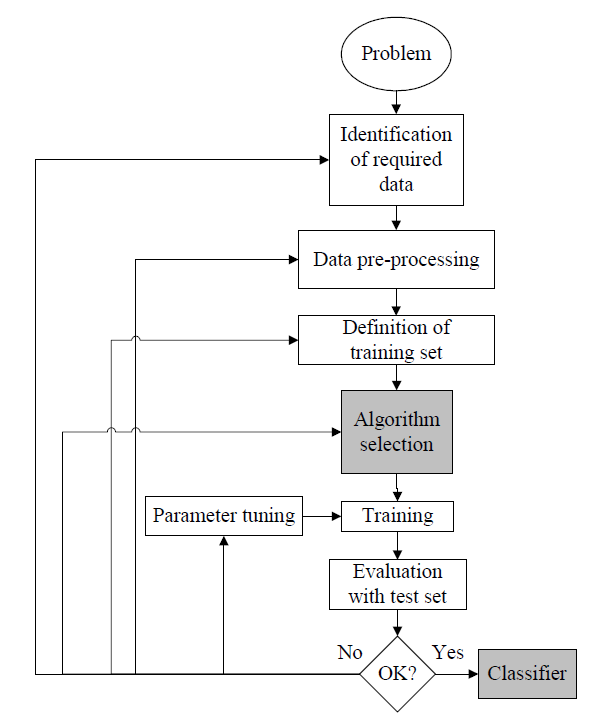
\includegraphics[width=0.8\textwidth]{images/chapter2/supervisedLearning.png}  
    \caption{General process of classification methods. From Kotsiantis et al. \cite{Kotsiantis2007}}
    \label{fig:supervisedLearning}
\end{figure}

\subsection{Decision Trees}

As described by Zaki et al. \cite{Zaki2014}, Decision Tree is a classification model which recursively partitions the data space into two parts. The split can be considered as a hyperplane parallel to one axis of the data space. The process repeats by dividing each new part into two smaller parts, and this process continues until each sub-part mostly contains items of only one of the target classes. The final result of this partitioning process
can be represented by a tree, where each node is a decision concerning which part an item belongs to, and the leaves represent one of the target classes.


As an example of the decision tree partitioning, consider the iris data set with 150 entries of three classes. The items are displayed in Figure \ref{fig:Recurcive2Decision1}, which plots their sepal length and width as X, Y axes. The partitioning process created six different regions, which are divided by lines instead of hyperplains, as in two-dimensional data space the hyperplanes can only have one dimension. Multiple regions might represent one of the targeted classes. The tree representation of the iris data space partition is shown in Figure \ref{fig:Recurcive2Decision2}.

\begin{figure}[!h]
    \hfill{\begin{minipage}{\dimexpr \textwidth-2\fboxsep-2\fboxrule}% maximum allowed
            \centering
            \subfigure[Recursive Splits]{
                \label{fig:Recurcive2Decision1}
                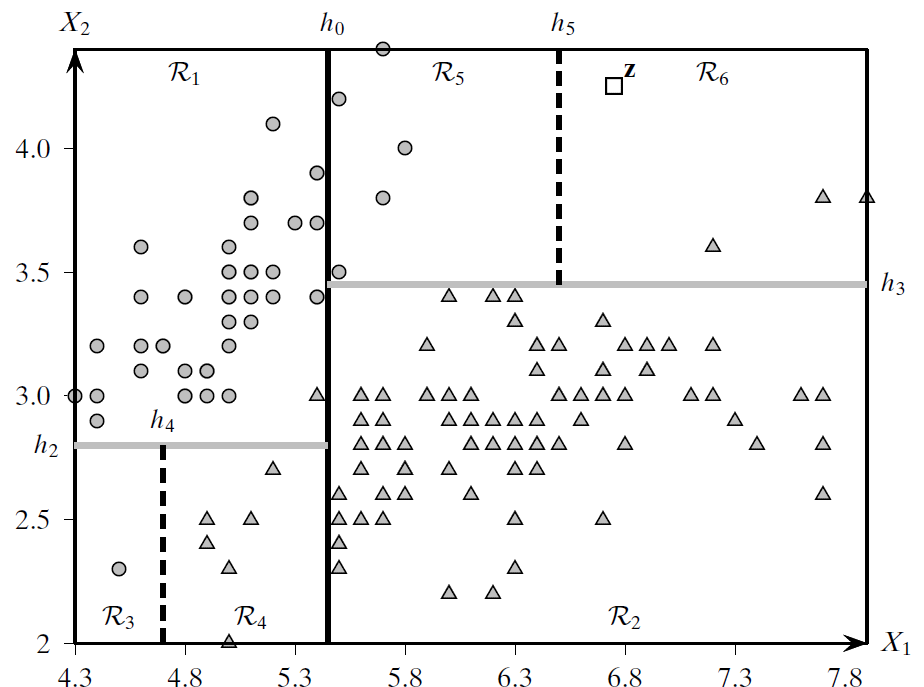
\includegraphics[width=0.8\textwidth]{images/chapter2/RecursiveCut.png}
            }\\
            \subfigure[Decision Trees]{
                \label{fig:Recurcive2Decision2}
                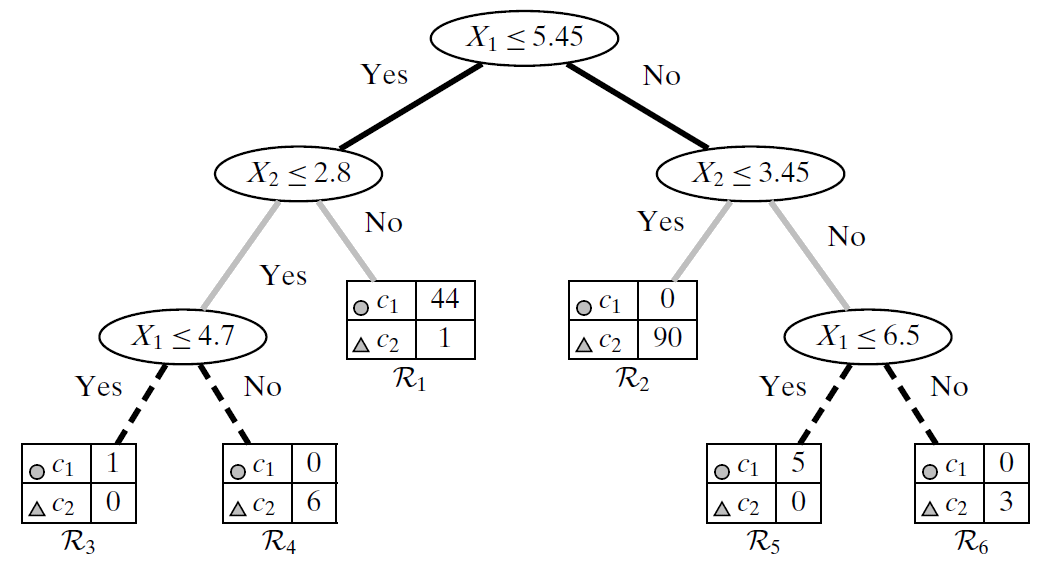
\includegraphics[width=0.8\textwidth]{images/chapter2/DecisionTreeExample.png}  
            }

    \end{minipage}}
    \caption{Decision trees representation for splitting items of the data by creating hyper-plains which are parallel to one of the axes. 
        (a) A two dimensional data set has been split recursively to differentiate between elements of different classes.
        (b) A tree representation for the values of the class limits.
        From Zaki et al. \cite{Zaki2014}}
    \label{fig:Recurcive2Decision}
\end{figure}

C4.5 might be one of the most famous decision tree algorithms for classification \cite{Wu2008}. C4.5 is build on ID3, both of which were introduced by Quinlan \cite{Quinlan2014}. This algorithm relies on information gained to create its tree for classification. In this algorithm attributes with higher normalised information gain are used for decide the splits in the data. The the next highest attribute is used for subpartitioning the data recursively \cite{Quinlan2014}.

This algorithm is superseded by a new version C5.0, which is more efficient as it uses less memory and functions more efficiently and effectively, generating a smaller and more concise decision tree, while it is more general as it can classify more data types than its predecessor. It also incorporates boosting, which means multiple classifier trees can be generated and they will vote for predicting items' classes. Boosting is a bootstrap aggregate (bagging) mechanism which may improve the stability and accuracy of the final result of the classifier \cite{Wu2008}. The last aspect of the algorithm is similar to what is provided by Random Forest algorithm, which creates many decision trees from random subsets of the training data \cite{Breiman2001}.

C4.5 has two drawbacks \cite{Hothorn2006}, the first of which is overfitting, which might be solved by pruning the decision tree to be more general. Two types of pruning can be done on the tree pre-pruning and post-pruning. Pre-pruning is the operation of preventing particular branches from growing when information becomes unreliable. Post-pruning is the operation of cutting branches of a fully grown tree to remove unreliable parts. The second drawback originates from the very nature of the algorithm by selecting attributes with the highest information gain value. This process will become bias to the attributes with a large number of values.

Conditional Inference Tree (Ctree) was introduced by Hothorn et al. \cite{Hothorn2006} to overcome the attribute bias of the information gain based algorithms. This algorithm uses significance to select covariants of attributes. The significance is determined through P-value which is derived from ANOVA F-statistics. During the training phase, all data permutations will be tested to calculate the p-value.

\subsubsection{Rule-Based Classification}

A rule-based classifier uses a set of rules to classify items in a data set. The rules are formalised in the form of IF-THEN clause. The conditions of the IF clause represent the rules that an item should fulfil to be accepted as a particular class. If the rules are ordered and have priority they can be represented in nested IF-THEN-ELSE clauses and might be called decision lists \cite{Witten2011}. 

Figure \ref{fig:ruleBased}a shows a simple data set with items labelled \textbf{a} or \textbf{b}. We can produce multiple variations of rules to classify items in this data set. It is possible to filter out all class \textbf{a} items first then all others remaining will be class \textbf{b}:
If x $>$ 1.4 and y $<$ 2.4 then class = \textbf{a}\\
Otherwise class = \textbf{b}\\

Conversely, if b class items are filtered out the remaining items will be classified as \textbf{a}:
If x $\leqslant$ 1.2 then class = \textbf{b} \\
If x $>$ 1.2 and y $\leqslant$ 2.6 then class = \textbf{b}\\
Otherwise class = \textbf{a}\\


In most cases, rule-based classification systems and decision trees can be used interchangeably; C4.5 provides both decision trees and classification rules \cite{Wu2008}. A decision tree representing the rule-based classifier is shown in Figure \ref{fig:ruleBased}b. The rules above and the decision tree can be considered as an equivalent classifiers, but most of the time people prefer rule-based classifiers on decision trees as they are more intuitive for human understanding \cite{Witten2011}, due to being simpler and more concise \cite{Wu2008}.


\begin{figure}[!h]
    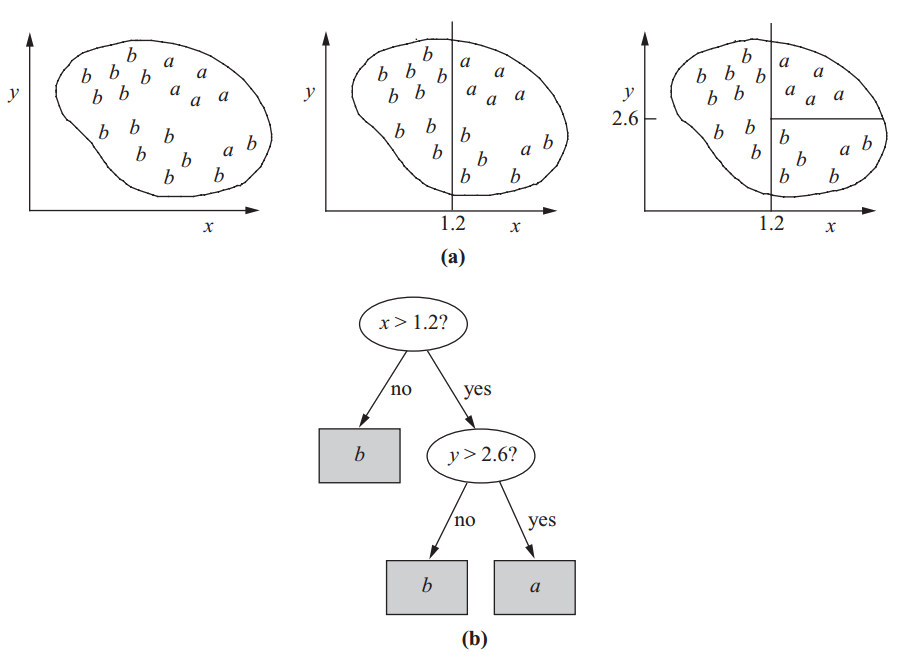
\includegraphics[width=1\textwidth]{images/chapter2/rulebased.png}  
    \caption{Classifying same data set using both rules and a decision tree.
        (a) A two dimensional data sets with items of two classes.
        (b) A tree representation for a rule based classification.
        From Witten et al. \cite{Witten2011}}
    \label{fig:ruleBased}
\end{figure}

Various methods are used to generate rule-based classifiers in different fields of application. The remainder of this section presents more effective samples of these works with a brief explanation of their methodologies.

Rodriguez et al. \cite{Rodriguez2012} used rule-based classification to classify power quality disturbances of signals. They used S-transform to extract features from signals, as this transform can generate variable window size with the ability to preserve phase information during decomposition \cite{Chen1996}. They used leaner and parabolic lines to separate between classes. The separation line is produced using a heuristic function to guarantee maximisation of the number of correctly classified signals from the provided training set.

Chung et al. \cite{Chung2002} use a two-stage classification method to classify power line signals, in the first of which they used a rule-based classifier to differentiate interrupt signals from others, which were then further classified using Hidden Markov Model classifier. The rules of the first stage classifier are created by domain experts relying mainly on the IEEE standards for signal interruption conventions, thus this classifier does not require a training set, as it is a static set of rules that can be calculated directly.

McAulay et al. \cite{McAulay1994} used genetic algorithms to create rule-based systems to identify alphabetical numbers. The system uses a random rule generator to create initial rules, which are enhanced through multiple generations by adjusting the initial rules. However, they notice that genetic algorithms might override even good rules which can identify specific characters. To prevent overriding rules, they introduced the concept of remembering rules for a long time if they succeeded to identify the training set example correctly.

Orriols-Puig et al. \cite{Orriols-Puig2009} used an evolutionary algorithm to create a rule-based classification system in which the system initiates with a set of classifier rules, then evolves online with the environment (new training items) to produce an accurate classification model. They proved that their classification method outperforms other methods (including support vector machine) in classifying data sets with imbalanced class ratios.

Nozaki et al. \cite{Nozaki1996}used fuzzy systems to create a rule-based classifier. Generating fuzzy rule-based classification system requires two phases, first partitioning the patron space into fuzzy subspaces and then defining a fuzzy rule for each of these. Nozaki et al. used a fuzzy grid introduced by Ishibuchi et al. \cite{Ishibuchi1992} with triangle-shaped membership function to generate fuzzy rules from fuzzy subspaces. To enhance the classification results they introduced two procedures, error correction-based learning and significant rule selection. Error correction-based process increases and decreases the procedure of increasing or decreasing rule certainty according to its classification of the items; if a particular rule correctly classified an item its certainty will increase, otherwise, it will decrease accordingly. Significant rule selection is a mechanism to prune unnecessary rules to construct a compact set of a fuzzy rule-based classifier.

As demonstrated above, many domains of computer science and machine learning are used to generate and optimise rule-based classification systems, including expert systems, genetic algorithms, evolutionary algorithms and fuzzy systems. While these classifiers are efficient and effective methods to classify underlying data sets, they require a training data set for rule generation and optimisation. This means a sufficient amount of correctly labelled samples should be available to cover all or most of the aspects and possibilities of situations and characteristics that have to be classified.

The availability of the training data set might not always be an option due to the fact that labelling items is a tedious and laborious undertaking requiring a extensive periods of professionals' valuable time. Experts might know the general rules for classifying items but they cannot identify the attributes of the classes individually due to the complexity of the underlying data sets. Moreover, domain experts might not quite agree on the fine differences between classes, so that it is hard to have a general single view for classifying items in the data set (such as in public goods games case study).

After the training stage these methods create a list of rules that represent the final rule-based classifier model, which might not cover all different opinions for nuanced cases of the classification (i.e. after the training stage, the classifier might lack the required generalisation). As noted previously, the generalisation problem might be solved by using rule pruning \cite{Nozaki1996}. However, this generalisation can be called local, as it depends on the training data, which is probably classified and labelled using expert single views.

Another aspect which is lacking in the presented methods is that they do not consider the classification of temporal data sets, as demonstrated in later sections. However, these methods also require training samples.



\subsection{Support Vector Machine}

\acrfull{svm} is a binary parametric classifier that classifies items by creating a hyperplane between classes. This algorithm tries to find an optimum position for the hyperplane so that it splits the classes with the maximum margin between class items and minimum empirical risk. The items on the edges of the margin are called support vectors, as each item can be seen as a vector. An example of an SVM classifier's hyperplane is shown in Figure 2.4. It can be noticed that in a two-dimensional data set the hyperplane is represented as a line \cite{Muller2001}.

\begin{figure}[!h]
    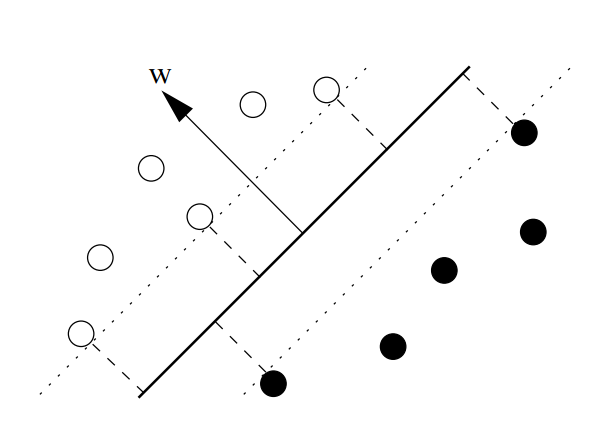
\includegraphics[width=0.6\textwidth]{images/chapter2/SVM.png}  
    \caption{Hyperplane of support vector machine between items of two classes showing vector $w$ and points on the dotted lines are support vectors. From Muller et al. \cite{Muller2001}}
    \label{fig:svmClassifier}
\end{figure}

Assume $D = \{(x_i, y_i)\}^n_{i=1}$ is a data set to be classified. The data set has n items in d dimensions, and each item has a set x of d attributes and y as a class label. For two classes we can assume that y can have one value of 1 or -1. The SVM's hyperplane $h(x)$ equation is defined as $h(x) = w^Tx+ b$. In this equation, w is a d dimensional weight vector and b (bias) is a scalar. The points on the hyperplane equal to 0 ($h(x) = 0$), so that for any $x_i$ if $h(x_i) > 0$ then $y_i = 1$ and if $h(x_i) < 0$ then $_iy = -1$ \cite{Zaki2014}. 

One of the advantages of SVM is that it can use kernel trick. For a data set with nonlinear separation between classes, we can map the d-dimensional items $x_i$ of input space into a high-dimensional feature space using a nonlinear transformation function \cite{Zaki2014}. 


SVM has been used as an elementary stage to create rule-based classifiers. Nunez et al. \cite{Nunez2006} used rule extraction mechanism to extract rules from an SVM model generated via training samples. The rules are constructed using multiple of ellipsoid equations. While these rules might present a good visual illustration for the rules, especially for two-dimensional spaces, these equations have mathematical forms so that the generated rules are not intuitive and easy to understand as stand alone rules. Moreover, the ellipsoids are not one-to-one maps for the actual hyperplanes of SVM, so the rule-based classifiers are not as efficient as their SVM counterparts and they have a higher error rate.



\subsection{K-Nearest Neighbours}
The \acrfull{knn} classifier is a nonparametric lazy classifier. In nonparametric classification the algorithm does not assume any specific distribution for the data sets. Lazy classifiers do not generalise the classification model and calculate the class of the item at the time of testing instead of training, which makes training very efficient by reducing the cost of testing time \cite{Wettschereck1997}. 

KNN estimates items' classes according to their nearest neighbours. The majority of the K nearest neighbours decide the class of the input item. An odd number of for K is selected (between 3 to 9) to prevent ties. The nearest neighbours are decided using one of the distance measures (e.g. Euclidean distance), as shown in Figure \ref{fig:KNN} \cite{Zaki2014}. 

\begin{figure}[!h]

    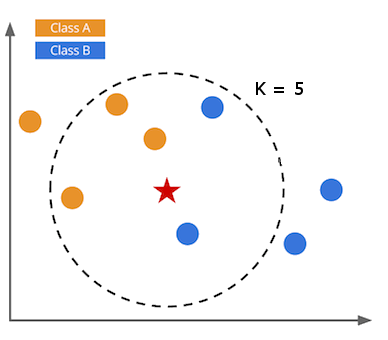
\includegraphics[scale=0.9]{images/chapter2/KNN.png}
    \caption{K-Nearest Neighbour Classification with K = 5}
    \label{fig:KNN}
\end{figure}

To prevent attribute bias due to different magnitudes of values it is strongly preferred to normalise all attributes before classification. Non-numerical attributes can also be used with KNN classification, similar attributes with the K neighbours have zero distance, and different attributes have the distance of 1 \cite{Zaki2014}. 

While this classification algorithm is different from rule-based classifiers, we used a variation of this classification for temporal attributes, as explained in chapter six, as a comparison with our proposed classification algorithm to test the performance difference between the algorithms.


\subsection{Classification Performance Measures}


Multiple methods exist to measure the performance of a classification algorithm and classify a data set into two classes, positive and classified. The terminology was developed in the medical field, where positive denotes the presence of a disease and negative indicates its absence \cite{Fawcett2006}. 

In a test data set D with n instances, a classifier tries to identify the class of instances for binary classifiers, whereby four possibilities exist. These possibilities for any classifier can be demonstrated as a confusion matrix, which is shown in Table \ref{tab:confusionMatrix}, and explained below \cite{Zaki2014}:

\begin{itemize}
    \item \acrfull{tp}: Number of correctly identified positive cases by the classifier.
    \item \acrfull{fp}: Number of incorrectly identified cases as positive but their true labels are negative.
    \item \acrfull{tn}: Number of correctly identified negative cases by the classifier.
    \item \acrfull{fn}: Number of incorrectly identified cases as negative but their true labels are positive.
\end{itemize}

\begin{table}[!h]
    \centering
    \begin{tabular}{l|l|c|c|c}
        \multicolumn{2}{c}{}&\multicolumn{2}{c}{True diagnosis}&\\
        \cline{3-4}
        \multicolumn{2}{c|}{}&Positive&Negative&\multicolumn{1}{c}{Total}\\
        \cline{2-4}
        \multirow{2}{*}{Screening test}& Positive & TP & FP & $a+b$\\
        \cline{2-4}
        & Negative & FN & TN & $c+d$\\
        \cline{2-4}
        \multicolumn{1}{c}{} & \multicolumn{1}{c}{Total} & \multicolumn{1}{c}{$a+c$} & \multicolumn{1}{c}{$b+d$} & \multicolumn{1}{c}{$N$}\\
    \end{tabular}
    \caption{Confusion Matrix}
    \label{tab:confusionMatrix}
\end{table}

To measure the overall performance of a classifier directly from the confusion matrix we can calculate the accuracy and error rates. The accuracy of a classifier is the fraction of correctly classified instances so that: $Accuracy = \frac{TP + TN}{n}$. In contrast, the fraction of all misclassified instances comprise the 
error rate which is: $Error Rate = \frac{FP + FN}{n}$ \cite{Fawcett2006}.

To measure class-specific performance we can use recall and precision. Recall is the ratio of correctly predicted number of a class labels to the real number of instances of that class in the data set. Recall for the positive instances in the data set is called sensitivity. The sensitivity is the ratio of true positive to the real number of positive cases in the data set so that $sensitivity = \frac{TP}{TP + FN}$. Precision is a class-specific accuracy; it is the ratio of the number of correctly predicted instances of a class to the number of predicted instances of the same class. A specific case of precision for the negative class is called specificity. The specificity is the ratio of true negative to the real negative cases in the data set so that $specificity = \frac{TN}{TN + FP}$ \cite{Fawcett2006}.

For a classifier, there is a trade-off between recall and precision; maximising one of them might cause the other to decline. Consequently, measures are introduced to overcome this problem and create a balance between these two measures. F-measure is computing the harmonic mean of the classes' recall and precision \cite{Zaki2014} so that:
\begin{equation*}
    F=\frac{2}{\frac{1}{precision} + \frac{1}{recall} } = \frac{2 \times precision \times recall}{precision + recall}
\end{equation*}


\acrfull{auc} of \acrfull{roc} is a measure used to calculate the performance of machine learning algorithms such as classification \cite{Bradley1997} . The ROC curve is a graph of the true positive and false positive rates of the predicted classifier's result compared to the real class for each item. Figure 2.6 shows ROC curves for different algorithms with various performances. AUC is the area under the ROC curve plotted as a performance result of the classifier. Methods of calculating AUC vary according to the nature of application and available data. The multi-class AUCs are calculated using the equations of \cite{Hand2001}. $auc = \frac{2}{c(c-1)}\sum aucs$. Where c is number of classes and aucs is a set of auc between any two classes.

\begin{figure}[!h]
    
    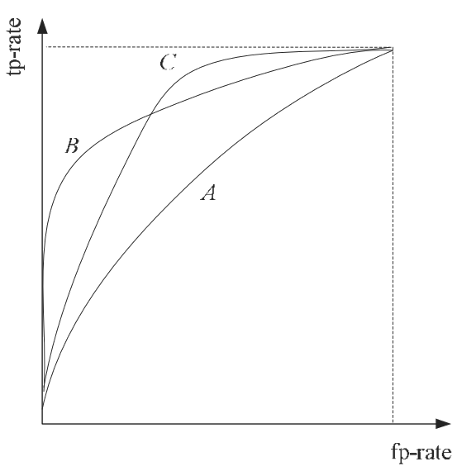
\includegraphics[scale=0.4]{images/chapter2/AUC.png}
    \caption{Receiver operating characteristic (ROC) curves for various classifiers. From \cite{Dietterich2010}}
    \label{fig:ROC}
\end{figure}

\section{Clustering}

Unsupervised machine learning methods aim to find patterns or groups (clusters) in data sets so that the most similar items in the data set will be gathered in the same cluster, and dissimilar items will be in different clusters. The task of clustering is required in many fields, especially when little information is known about the data sets, and field experts have few assumptions about it. Examples of fields in which clustering is required include data mining, pattern recognition, decision making, document retrieval and image segmentation \cite{Jain1999}.

In this thesis, multiple clustering algorithms are used to cluster items of each time point in temporal data. Each time point was used separately, so there is no time effect on the clustering because each time point is treated as a separate data set. This clustering process is part of the proposed method to measure changes over time in temporal data (as presented in chapter four). We also used clustering multiple temporal clustering algorithms as a comparison with our proposed classification method (chapter six).

Figure \ref{fig:Clustering} shows the main steps of a clustering method. It can be noticed that unlike supervised methods, clustering methods do not have training data set to generate their model. Instead, they entirely depend on the given features of the items in the data set to group them into clusters. 

\begin{figure}[!h]
    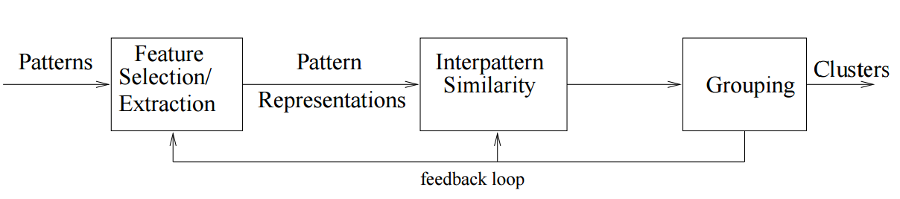
\includegraphics[scale=0.4]{images/chapter2/ClusteringSteps.png}
    \caption{General steps of clustering methods. From \cite{Jain1999}}
    \label{fig:Clustering}
\end{figure}

The first step in any clustering task is feature selection/extraction. Feature selection refers to selecting a group of features (attributes) of the original data set which are most effective and representative for the instances or items which have to be clustered. Feature extraction is the process of deducing new features by transforming existing ones to obtain more effective features. The aim of feature selection and extraction is to obtain an effective and efficient clustering method by creating better quality of clusters in shorter computation time \cite{Jain1999}.

The second step is detecting pattern similarity by finding the distances between items in the data set. Multiple distance measures are available to measure the similarity between any two points in a hyperspace of features like Euclidean and Manhattan distances and correlation coefficients \cite{Jain1999}.

The next step is the actual clustering process to identify patterns in data sets using one of the available clustering algorithms. There are multiple clustering algorithms which can be classified into four types Centroid-based clustering, Density-based clustering, Fuzzy clustering and Hierarchical clustering \cite{Zaki2014}.

The last step is feedback or clustering evaluation. There are many ways to evaluate the results of clustering algorithm, including using external clustering validity indices to compare generated clusters with the true classes of the items or using internal clustering validity to evaluate the structure of the clusters and the similarities between items of one cluster compared with dissimilarities with items of different ones \cite{Jain1999, Zaki2014}.


\subsection{Centroid-Based Clustering}

Centroid-based or representative-based clustering is a method of finding the best k clusters of items in the D data set. Each cluster contains a representative point which might be called centroid \cite{Zaki2014}. Two examples of centroid-based clustering discussed below are K--means and PAM clustering methods.

\subsubsection{K--means Clustering}

K--means clustering is partitional-based and produces k clusters, minimising the distance between the centre of the cluster and cluster members. The criterion used to calculate the quality of the cluster is the sum of squared errors to the centroid. The aim of the algorithm is to find centroids that minimise the sum of squared error for all clusters \cite{Zaki2014}. 

The process starts by assigning k random items as centroids, after which each item is appointed to a cluster with the nearest centroid to it. The location of the centroid is updated according to the existing items in the cluster. The process of assigning instances to clusters and updating centroids is reiterated until convergence (i.e. the centroids stabilise) or a fixed number of iterations has been reached \cite{Jain1999}.  

K--means works as a greedy optimisation algorithm so that it might converge to local optima \cite{Zaki2014}. Moreover, using the sum of squared error as a criterion for finding better clusters makes K--means sensitive to outliers, so that extreme values might distort the distribution of the data \cite{Jain1999}. 

\subsubsection{PAM Clustering}

\acrfull{pam} clustering is another centroid-based technique, but unlike K--means it uses actual instances of the data set as representatives for the clusters instead of virtual centroids. It uses a similarity measure to identify members of a cluster. The members most similar to a medoid are considered in the same cluster so that the sum of squared errors can be used with PAM algorithm to identify the quality of clusters \cite{Kaufman1990}.

Similar to K--means, PAM algorithm starts with random k set of medoids, then each instance is registered as a member of a cluster according to its similarity distance from the medoid. The sum of squared errors is calculated for the current set of medoids. In the original algorithm, different instances are selected as nominees for medoids to optimise the initial state, and the sum of squared errors is calculated according to the selected instances \cite{Kaufman1990}. If the selected instances perform better than the original set of medoids, then they will be replaced with the new ones. This process can be repeated multiple times until convergence. However, due to the large time requirement and complexity of this method, it is usually used only for small data sets, and for larger data sets a modified version of the original version is preferable to find optimum medoids in an acceptable time frame \cite{Ng2002}. 

\subsection{Fuzzy Clustering}

Fuzzy sets are used in fuzzy logic and can be considered as a generalisation of set theory. An element can be a member of a particular set or not in set theory, while in fuzzy set theory an element can have a gradual transition membership between sets. Hence, fuzzy clustering uses the fuzzy set to allow an instance to be in more than one cluster at the same time \cite{Wang2006}. 

The most well known and used fuzzy clustering is fuzzy c--means algorithm, developed by Dunn \cite{Dunn1973a} and later improved by Bezdek \cite{Jain1999} who introduced the concept of the fuzzifier parameter \textbf{m}. This parameter, also called 'fuzziness index', is used to control the fuzziness of the membership of each item in the data set. Usually, m = 2 is used without any particular theoretical basis for this choice. For m = 1 the fuzzy c--means will behave as k--means algorithm, and the fuzziness of the system increases with the larger value of m parameter \cite{Bezdek1981}. 

The fuzzy c--means algorithm has a similar approach as k--means algorithm. It requires a predefined number of clusters. Both algorithms start with random initialization of the cluster centres so c--means might have the same problem as k--means by converging to local optima. The result of the cmean algorithm is expressed as a membership percentage of each instance to the available clusters. This fuzzy membership clustering can be converted into hard clusters by choosing a cluster for each item with the highest membership ration \cite{Wang2006}.

\subsection{Hierarchical Clustering}

Hierarchical clustering is a method to group instances of a data set into a series of nested clusters or a tree of clusters called a dendrogram, which represents the similarity level between instances in the data set. An example hierarchical clustering is shown in Figure \ref{fig:Hira}. The figure shows a simple two-dimensional data set with three distinctive clusters. The data set is represented as in a hierarchical clustering model using a dendrogram. The dendrogram can be cut at any level (represented as a dotted horizontal line) to separate different patterns of the data set \cite{Jain1999}. The level of the cutoff line is subjective and may vary from one data set to another. Cutting a dendrogram from a higher level produces fewer patterns (clusters) \cite{Wang2006}.

\begin{figure}[!h]
    \hfill{\begin{minipage}{\dimexpr \textwidth-2\fboxsep-2\fboxrule}
            \centering
            \subfigure[Data set]{
                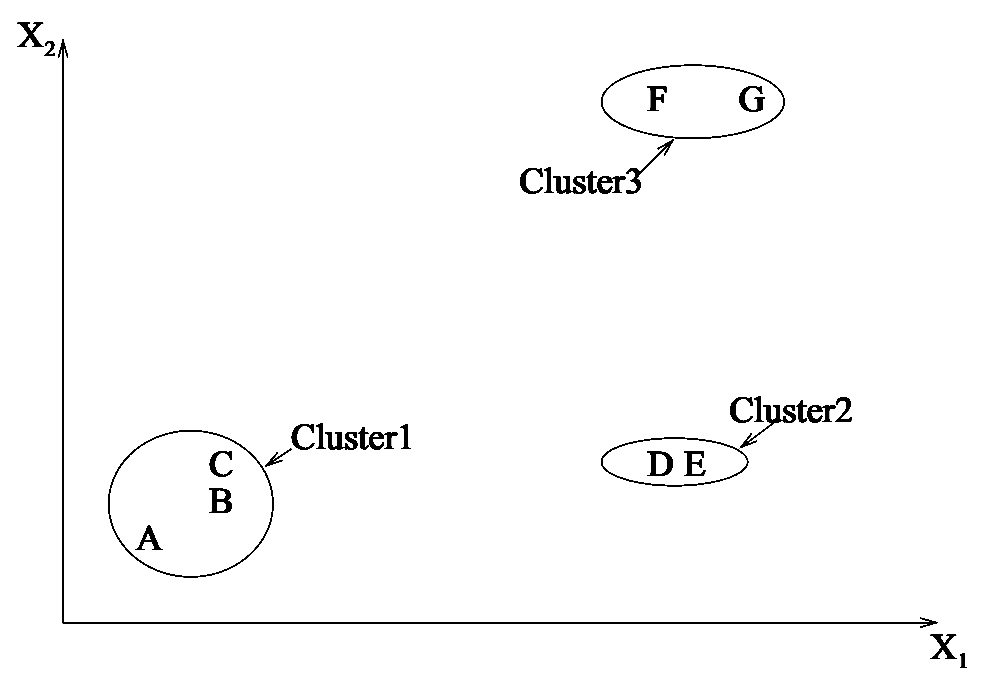
\includegraphics[width=0.7\textwidth]{images/chapter2/hira1.png}
            }\\
            \subfigure[Dendrogram of the data set]{
                
\includegraphics[width=0.7\textwidth]{images/chapter2/hira2.png} 
            }
            
    \end{minipage}}
    \caption{A simple data set with a possible dendrogram for hierarchical clustering algorithm. 
        (a) Two dimensional data set with three obvious different groups.
        (b) A dendrogram representation for a hierarchical clustering of the previous data set
        From \cite{Jain1999}}
    \label{fig:Hira}
\end{figure}

Based on the internal functioning of the hierarchical clustering algorithm, they can be divided into divisive and agglomerative types. The divisive method starts by assigning all instances into one cluster then partitions that cluster into two smaller clusters according to the similarities between instances. The process of sub-dividing each subcluster into another two clusters continues until each cluster contains single instance. In contrast, agglomerative hierarchical clustering starts by assigning each instance of the data set as a cluster, then starts to combine two most similar clusters into a single bigger cluster. This process is repeated recursively until a single cluster is achieved or a certain number of clusters are reached \cite{Zaki2014}.

Whether divisive or agglomerative approach is used, a prerequisite to begin clustering is a proximity matrix, a symmetric matrix containing the similarity between every point in the data set using a distance function. This matrix is updated after each iteration to reflect the status of the data set under the method of clustering. The distance function can be Euclidean, Manhattan or any other distance function \cite{Zaki2014}. Sections shows how time-based distance measures can be used to cluster temporal data sets.

To determine the similarity between clusters using proximity matrix in agglomerative method, one of the available linkage methods can be used \cite{Wang2006}:

\begin{itemize}
    \item Single linkage: calculates the minimum distance between any items of two different clusters.
    \item Complete linkage: calculates the maximum distance between any items of two different clusters.
    \item Average linkage: calculates the average distance between all items of two different clusters.
    \item Centroid linkage: calculates the distance between centre of two different clusters.
\end{itemize}

Due to the time complexity hierarchical clustering can not be used with very large data sets which can not fit the memory. Moreover, the nature of the algorithm do not allow to reconsider the previous steps of the recursive clustering operation (dividing or joining) in contrast with the other clustering technique which we see before \cite{Wang2006}. 


\subsection{Clustering Validation}

Many clustering methods exist to be used in different situations according to the underlying data to be analysed and clustered. There are many methods to assess clustering results and their initial configurations, which can be categorised into three main types: clustering tendency, cluster stability and cluster evaluation \cite{Zaki2014}. 

Clustering tendency or clusterability assesses the suitability of the data for clustering. The aim is to determine that the data has meaningful patterns to be clustered. The spatial histogram method for cluster tendency creates a histogram for the input data set and distance distribution by calculating the pairwise distance between data points. An example of non-clusterable data is uniform instances of a data set, as shown in Figure \ref{fig:uniformData} \cite{Zaki2014}. 

\begin{figure}[!h]
    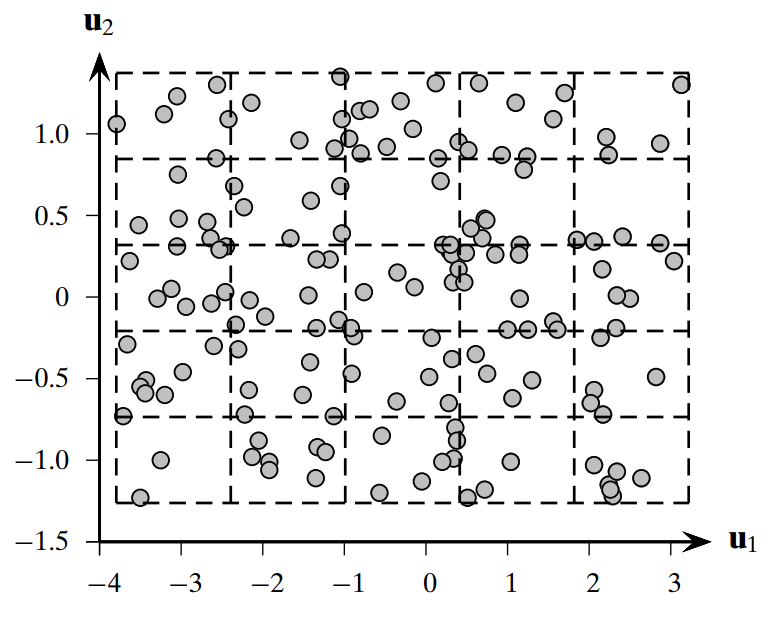
\includegraphics[scale=0.33]{images/chapter2/uniformData.png}
    \caption{An example of uniform data which can not be clustered. From Zaki et al.\cite{Zaki2014}}
    \label{fig:uniformData}
\end{figure}

Cluster stability is concerned with the initial parameters of clustering algorithms, like the number of clusters in K--means. The aim of this method is to determine the optimum initial parameters for the clusters, so that the cluster of different samples of data from the same underlying population guarantee comparable results. Methods of determining the stability of clusters include generating perturbed versions of the data set, using distance functions (e.g. Euclidean) and similarity measures like Rand index \cite{VonLuxburg2010}.

Clustering evaluation can use cluster validity indexes to evaluate the quality of the produced clusters. This task can be further divided into three categories \cite{Halkidi2002a, Halkidi2002, Zaki2014}:

\begin{itemize}
    
    \item \textbf{External}: External validation derives the estimation for the quality of the generated clusters from sources outside the data set. The most general case is using true labels of items, provided by field experts.
    
    \item \textbf{Internal}: Internal validation derives the estimation for the quality of the generated clusters using the structure of the data and the clusters. It computes the compactness of the clusters and the separation of clusters from each other.
    
    \item \textbf{Relative}: External validation compares between the results of two different clusterings for the same data set. The clusterings might be generated using different clustering algorithms, or the same clustering algorithm with different initial parameters.
    
\end{itemize}

The following subsections focus on the cluster validity indices, especially those used in this thesis.

\subsubsection{External Criteria}
External criteria validate the results of clustering based on some predefined structures of the data which is provided from an external source. The most well-known example of structural information is labels for the data provided by experts (called true classes). The main task of this approach is to determine a statistical measure for the similarity or dissimilarity between obtained clusters and labels \cite{Halkidi2002a, Rendon2011}. According to the methods incorporated in the external criteria, they can be divided into three types: pairwise measures, entropy-based measures and matching based measures \cite{Zaki2014}. 

As mentioned previously, the four types of classification guesses evaluation are true positive, true negative, false positive and false negative. These terms are used in the terminology of external cluster validity, especially when using pairwise measures, but with slightly different meanings to enable the evaluation of clusters in the same manner as classification \cite{Zaki2014}:
\begin{itemize}
    \item True Positives \textbf{TP}: Any two instances with the same label that are in the same cluster.
    
    \item False Negatives \textbf{FN}: Any two instances with the same label that are not in the same cluster.
    
    \item False Positives \textbf{FP}: Any two instances with different labels that are not in the same cluster.
    
    \item True Negatives \textbf{TN}: Any two instances with different labels that are not in the same cluster.
    
\end{itemize}

In this thesis, we use various external cluster validity indices to determine differences between a reference of behaviour for items in a temporal data and clusters of items in each time point. The method is discussed in more detail in chapter three and implemented in chapter four for public goods games and chapter six for stock market data. The used criteria in the thesis are listed below:

\textbf{Jaccard Coefficient: }
This coefficient is a pairwise measure representing the degree of similarity between clusters. With this coefficient, each cluster is treated as a mathematical set, and the coefficient value is calculated by dividing the cardinality of the intersection of the resultant cluster with the prior cluster to the cardinality of the union between them \cite{Vendramin2010}:
\begin{equation*}
Jaccard = \frac{TP}{TP + FP + FN}
\end{equation*}

With a perfect clustering, when false positives and false negative equal to zero, the Jaccard coefficient value equals 1. This measure ignores the true negatives and only focuses on the true positives to evaluate the quality of the clusters \cite{Zaki2014}. 

\textbf{Rand Statistic: }
The Rand statistic measures the fraction of true positives and true negatives over all point pairs; it is defined as
\begin{equation*}
Rand = \frac{TP + TN}{N}
\end{equation*}
Where N is the total number of instances in the data set. This measure is similar to Jaccard Coefficient, so its value equals 1 in perfect clustering \cite{Zaki2014}.


\textbf{\acrfull{fm}:}
FM define precision and recall values for produced clusters \cite{Fowlkes1983}
\begin{equation*}
FM = \sqrt{prec. recall} = \frac{TP}{\sqrt{(TP + FN)(TP + FP)}}
\end{equation*}
Where $prec = \frac{TP}{TP + FP}$ and $recall = \frac{TP}{TP + FN}$. For the perfect clustering this measure equals 1 too \cite{Zaki2014}.



\textbf{\acrfull{vi}: }
This index measure is based on contingency table which is a matrix with $r \times k$ , where $r$ is number of produced clusters and $k$ is the number of externally provided clusters. Each element of this matrix contains a number of agreed instances between any two clusters of the externally provided and produced clusters. As introduced by Meila \cite{Meila2007a}, this index calculates mutual information and entropy between previously provided and produced clusters derived from the contingency table:
\begin{equation*}
VI(C,T) = 2H(T,C)- H(T)- H(C)
\end{equation*}
Where $C$ is produced clusters, $T$ is ground truth clusters, $H(C)$ is entropy of $C$ and $H(T)$ is entropy of $T$ \cite{Zaki2014}.




\subsubsection{Internal Criteria}
Internal criteria measure the 'goodness' of clusters for the data by extracting information from data and clusters alone, such as the compactness of data points inside one cluster and the separation of clusters from each other \cite{Rendon2011}. These criteria were used as part of the cost function, to determine the quality of the selected classification rules in each time point, and to compare different clustering algorithms' performances, as presented in chapter six.


\textbf{Dunn Index: }
This index calculates the ratio of minimum distance between clusters to the maximum distance between any two instances of the same cluster \cite{Dunn1973}:
\begin{equation*}
Dunn = min_{1\leqslant i \leqslant c} \left \{ min \left \{ \frac{d(c_i, c_j)}{max_{1\leqslant i \leqslant k(d(X_k))}} \right \} \right \}
\end{equation*}
Where $c_i, c_j \in c$ of size $m$ and the maximum distance can be computed from the mean or between all pairs. A larger value for Dunn index means, better clustering output, because it means that the closest instances between two clusters are larger than the distance between two farthest instances in the same cluster \cite{Zaki2014}.


\textbf{\acrfull{db}:}
This measure is introduced by Davies et al. \cite{Davies1979a}. It calculates intera cluster compactness and inter cluster separation by producing the ratio of spreading sample points around mean (i.e. variation) to the distance between mean of clusters \cite{Rendon2011}. 
\begin{equation*}
DB = \frac{1}{k} \sum_{i=1}^{k}\sum_{j=1}^{k}\max_{i\neq j }\left \{ \frac{s_{\mu_i} + s_{\mu_j}}{\delta(\mu_i, \mu_j)} \right \}
\end{equation*}
Where $k$ is number of clusters, $ s_{\mu_i}$ and $s_{\mu_j} $ are the spread of points around any two clusters cluster mean ''Centroid'', and $\delta(\mu_i, \mu_j)$ denotes the mean of both clusters.

A smaller value of this measure indicates better the clustering, as in such cases the clusters are well separated and each cluster is well represented by its mean; in other words, larger values mean better compacted instances in the clusters and clusters that are well separated from each other \cite{Zaki2014}.


\textbf{\acrshort{sd}: } This measure is introduced by Halkidi et al. \cite{Halkidi2000}. It calculates the average scattering for clustering and total separation among clusters. 
\begin{equation*}
SD = a \times Scatter + Distribution 
\end{equation*}
Where $a$ is a weighting factor equal to the maximum distance of two instances in the data set. The $Scatter$ indicates the average compactness of clusters. A smaller value of $Scatter$ is a signal for a compact cluster, and its the value increases for less compact clusters. The $Distribution$ is the measure of the total separation between clusters. A larger value $Scatter$ indicates better clustering and a smaller value of this term indicates greater proximity between clusters to each other. $Scatter$, and $Distribution$ have different ranges so that $a$ (the weighting factor) is important to maintain the balance between them. As SD measure is a total of $Scatterer$ and $Distribution$ so that the smaller SD value indicates better clustering \cite{Halkidi2000}.


\textbf{\acrshort{sdwb}:} This measure is introduced by Halkidi et al. \cite{Halkidi}. The S\_Dbw index is similar to SD index as it measures the intracluster and intercluster variances \cite{Rendon2011}. The definition of S\_Dbw indicates that both criteria of ''good'' clustering (i.e. compactness and separation) are properly combined, enabling reliable evaluation of clustering results. 
\begin{equation*}
S_Dbw = Scatter + Dens_bw
\end{equation*}
 As with SD, the $Scatter$ indicates the average compactness of clusters, smaller $Scatter$ value indicating a compact cluster, with an increased value for less compact clusters. Dens\_bw(c) indicates the inter-cluster density by calculating the average number of points between the clusters in relation with density within clusters. Thus a small value of Dens\_bw means good separation among clusters. As in SD, a smaller value of this measure is an indication of well defined clustering \cite{Halkidi}.


\subsubsection{Relative Criteria}

Relative criteria are used to compare between two clusterings with same data and clustering algorithm but different initial parameters, like number of clusters \cite{Halkidi2002}. These criteria mostly use internal clustering validity indices like Dunn index and Davies–-Bouldin Index to compare between clusterings' initial parameters \cite{Jain1988}. On the other hand Vendramin et al. \cite{Vendramin2010} proposed a novel method to compare relative criteria, using external cluster validity indices like Jaccard and Rand.



\section{Temporal Data Analysis}

Temporal data analysis is concerned with mining and analysing sequential data sets \cite{Laxman2006}. A sequential data set is ordered according to some index. A special case of sequential data is temporal data, which is ordered according to a time reference. According to Han et al. \cite{Han2006}, ''A time-series database consists of sequences of values or events obtained over repeated measurements of time.''. In this thesis, we use the terms ''time series'' and ''temporal data'' interchangeably. Sequential data sets can be used in applications to study protein order series, DNA sequence and lists of moves in a chess game. Examples of temporal data include stock market data and public goods game data set. Data streams can be considered as a special case of temporal data with an endless sequence of flowing data, such as satellite remote sensor, data from electric power grids and telecommunications data \cite{Han2006}.

In the following subsections we discuss methods to measure changes in temporal data as well as classifying and clustering them.

\subsection{Measuring Changes in Temporal Data}

Spiliopoulou et al. \cite{Spiliopoulou2006} introduced the \acrshort{monic} model, which finds cluster transition over accumulating data sets, providing an ageing function for clustering data that prioritises new records over old ones and eliminates records older than two time points. Matching for clusters in one time point to the next one is carried out by passing a threshold that determines normalised maximum number of records that exist in both matched clusters in the two time points. This model defines two kinds of transitions, external and internal. In external transition, clusters may survive, split, be absorbed, disappear or emerge, while in internal transition clusters can change in size, compactness or location.

According to MONIC, each cluster has a lifetime, which is the number of time points throughout which it can survive. Longer cluster lifetimes enable more predictable clustering while short lifetimes lead to volatile and unpredictable clustering.


It can be observed that this model relies on \gls{accumulateddata} over time to detect cluster matches, therefore it cannot be used with non-accumulated data. Moreover, it emphases the measurement of cluster changes and cannot detect changes in cluster membership for individual items clustered over time points.



Gunnemann et al. \cite{Gunnemann2011a} introduced a method which traces cluster evolution as change in behaviour types indicated by the value of objects (e.g. persons) in high-dimensional data sets. Different types of mapping function were introduced to map clusters according to their values in different dimensions and subspaces instead of object identifier.

Using this method cluster evolutions were detected and counted in the forms of emerge, disappear, converge and diverge. Moreover, the loss and gain of dimensions of subspace clusters were calculated.

This method counts the number of various changes that occur to clusters of any high dimensional data set, but it lacks to any mean by which to quantify the changes themselves; in other words, there is no indication of the quantity of change that happens to any cluster in two consecutive time points.



Hawwash et al. \cite{Hawwash2012a} proposed a framework for mining, tracking and validating clusters in a data stream using statistical cluster measures like cardinality, scale and density of clusters to detect milestones of clusters change and monitor the behaviour of cluster.

This framework targets accumulative clustering on data streams, but instead of using fixed-time window for clustering it uses milestones to detect the next-best clustering time.

Hawwash et al. \cite{Hawwash2012a} used a linear model in their metrics, which cannot represent real-life situations. They made this concession due to time limitations and the memory complexity of higher degree models. With some enhanced models this method could be profitably used to determine critical time points in the data stream clustering and to track clusters behaviour in general using statistical measures for representative numbers pertaining to the situation of clusterings.



Kalnis et al. \cite{Kalnis2005} introduced a method to discover moving objects in the snapshots of spatio-temporal data using cluster mapping function, treating clusters as sets and calculating the cardinality ratio of intersection for each two time constitutive clusters over their union; if the ratio passes a certain threshold the cluster is considered to be a moving cluster.

This method detects move in overall clusters and provides visual aids enabling human experts to grasp changes in the underlying data \cite{Ntoutsi2011, Bottcher2008}. This method is excellent for tracking moving cluster change \cite{Ntoutsi2009} , but it still lacks a method to quantify the magnitude of change for overall clustering objects.




Aggarwal \cite{Aggarwal2005} introduced a new method to detect changes for single clusters in the data streams that also works for snapshots of data as special cases. This method uses forward and reverse time slice density estimates based on fixed length time window to calculate velocity density at time and space dimensions.

By calculating velocity density three types of change can appear on the clusters in evolving data streams: 1) they may coagulate if the value passed a user specified threshold; 2) they may decay if the value does not pass the threshold; or 3) they may shift their location to another. This method is particularly germane to visually understanding the characteristics of underlying data.


In summary, the previously mentioned methods: 1) are mostly designed to work with data streams or snapshots of spatio-temporal data sets; 2) detect changes inside data by monitoring cluster change in terms of split, absorbed, disappear and emerged etc., which is a good indication for detecting existence of change, but which does not specify the magnitude of change. Our aim is to create a simple factor (scalar) to express the magnitude of change among members of clusterings in temporal data sets.


\subsection{Temporal Classification}

Temporal and sequence classification is an automatic system that assigns one of the predefined classes to the time series or sequence input \cite{Laxman2006}. Many temporal classifications have been introduced that reuse traditional classification algorithms in terms of criteria and measurements crafted for temporal data. Three main methods exist for classifying temporal data set: distance--based, feature extraction--based and model--based \cite{Amr2009,Laxman2006}.

Wang et al. \cite{Wang2005} proposed a rule-based classification method for categorical and high-dimensional data sets that rely on calculating frequent item sets using frequent pattern mining and association rules, then using the highest confidence sets covering rules for grouping according to rule heads (class labels). This method has been found to result in an efficient and accurate rule-based classifier, but it might produce a very large number of rules, as they are extracted from association mining, which might be hard for humans to follow and comprehend. Moreover, to create the frequent item test, it is required to have training data sets, which might be expensive and labour intensive to acquire and deploy.

It is possible to use traditional classification algorithms (non-temporal) to classify temporal data set by using distance measures specially designed to evaluate distances in a temporal data set. Many temporal supervised and unsupervised algorithms use \acrfull{dtw} \cite{Berndt1994} to align between two sequences or time series and find the distance between them. This method was originally used in speech recognition to identify human speech patterns \cite{rabiner1993fundamentals}. 
 

\begin{figure}[!h]
    \centering
    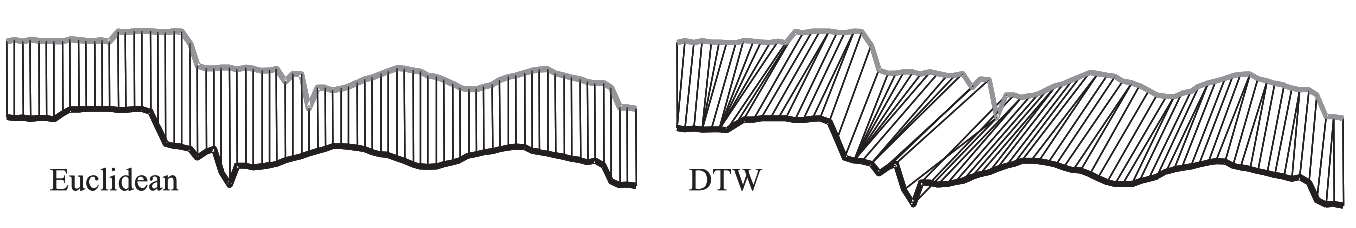
\includegraphics[width=1\textwidth]{images/chapter2/DWtvsEuclidean.png}
    \caption{Difference between time alignment and Euclidean distance of two time series. Aligned points are indicated by arrows. From Keogh et al. \cite{Keogh2005}}
    \label{fig:DWtvsEuclidean}
\end{figure}


Dynamic time wrapping tries to find the best match between two time series to calculate the smallest distance between them, unlike Euclidean distance, which uses the one-to-one mapping between the same time points regardless of any time shift. Figure \ref{fig:DWtvsEuclidean} compares these two distance measures. Dynamic time wrapping creates wrapping matrix which consists of Euclidean distances between every two points in both time series; then a local cost function finds the shortest path between two time series that represents the best match. Dynamic time wrapping has been implemented successfully in numerous temporal classification and clustering methods, but it has a drawback in using heuristic methods, which are inefficient due to searching for the best path in the wrapping matrix \cite{Keogh2005}. The wrapping matrix and time wrapping distance between two time serris are shown in Figure \ref{fig:timewrapIllustration}.

\begin{figure}[!h]
    \centering
    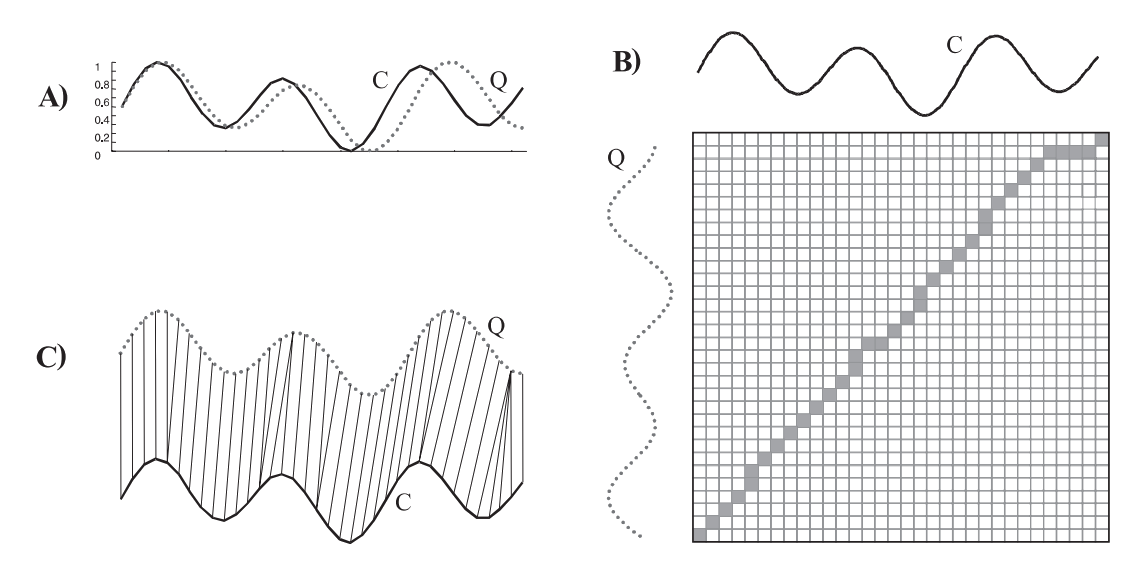
\includegraphics[width=1\textwidth]{images/chapter2/DTWIlustration.png}
    \caption{Calculating the distance between two time series using wrapping matrix. 
        (a) Two similar but out of phase sequences. 
        (b) Finding the optimal path (minimum distance) between the sequences which causes time wrap alignment between different time points of them.
        (c) The resulting alignment.
        From Keogh et al. \cite{Keogh2005}}
    \label{fig:timewrapIllustration}
\end{figure}



\begin{figure}[!h]
    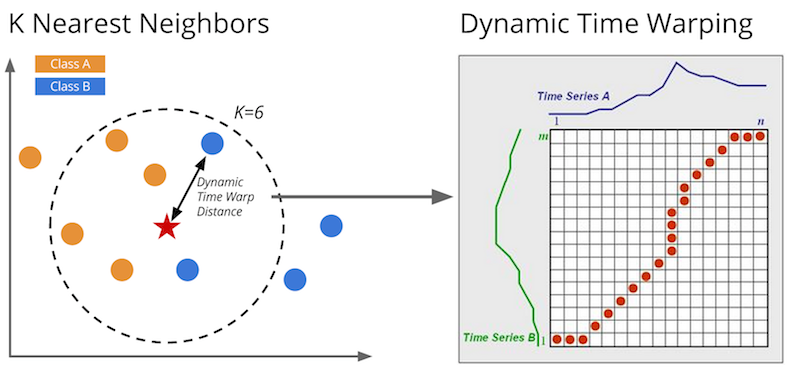
\includegraphics[scale=0.8]{images/chapter2/KNN_Temporal.png}
    \caption{K-Nearest Neighbour using dynamic time wrapping for time series classification. From Regan \cite{Regan2014}}
    \label{fig:KNN_Temporal}
\end{figure}

Distance-based K-Nearest Neighbours classification method (KNN) is used with temporal and sequential data with Euclidean distance measure \cite{Wei2006}. However, for complex time series, Euclidean distance is sensitive to the time fluctuation; thus DTW has been used \cite{KajanLaszl2006}. Figure \ref{fig:KNN_Temporal} illustrates temporal KNN operation.




It is possible to use feature extraction in order to extract useful features from time series so that it becomes possible to use traditional classification methods to classify temporal data. Agrawal et al. \cite{Agrawal1993a} proposed the use of the \acrfull{dft} to transform a sequence from the time domain to the frequency domain. Using DFT allows selection of the most important frequencies then representing them back in the original dimensional space. The DFT has an important property as it can ignore shifts and find similar sequences because the Fourier coefficient is invariant for shifts.


Chan et al. \cite{Chan1999} used \acrfull{dwt} to translate each time series from the time domain into the time/frequency domain. This transformation is linear as it changes the original time series into various frequency components in a lossless transformation. The sequence is then represented by its features, expressed as wavelet coefficients. Only a selected number of coefficients are necessary to represent the original time series, which allows a better and efficient use of the available classification algorithms.


Douzal-Chouakria et al. \cite{Douzal-Chouakria2012} used classification trees to classify time series data by introducing new splits for the tree nodes using time series proximities, relying on adaptive metrics considering behaviours and values. Other methods use SVM as a temporal data classifier using different kernels \cite{Sitaram2007}.

Model-based classifiers can also be used for temporal and sequential classifications, like Naive Bayes sequence classifier \cite{Tseng2009} and Hidden Markov Model \cite{Oates1999}. In the training step, the parameters of the model are created and trained depending on some assumptions, and a set of parameters describing probability distributions. In the classification step, a new sequence is assigned to the class with the best possible similarity \cite{Xing2010}.

\subsection{Temporal Clustering}

%\cite{Hawwash2012a}
%\cite{WarrenLiao2005}

%http://stats.stackexchange.com/questions/132780/bisecting-k--means-using-dynamic-time-warping

%http://stats.stackexchange.com/questions/131281/dynamic-time-warping-clustering


Clustering is an unsupervised machine-learning method whose goal is to find natural groupings (clusters) of instances in data sets. All clustering methods strive to detect compacted clusters by maximising the total sum of inter-cluster distance and minimising the total sum of the intra-cluster distance between instances \cite{Esling2012}. The distance can be measured using Euclidean distance, DTW distance, or any other similarity measures.


Jebara et al. \cite{Jebara2007} used \acrfull{hmm} to cluster time series data, while Oates et al. \cite{Oates1999} compared two methods for clustering time series data sets, first using HMM alone and then using DTW with HMM.DTW returns the minimised area between two time-series variables, which can be used as a similarity measure between them. They concluded that using DTW enhances the efficiency and effectiveness of the clusterings of the time series data set.


Rodrigues, Gama and Pedroso \cite{Rodrigues2008} used hierarchical clustering to cluster time series data sets. A hierarchical clustering method works by grouping item into a tree of clusters. The tree can be generated in two ways, either by starting from single items then agglomerating them into a higher structure, or starting from the entire data set and dividing it until ends up with single items in each branch of the tree \cite{WarrenLiao2005}. Another method used a scaled-up version of DTW \cite{Keogh2000} with hierarchical clustering, which calculates the distance between temporal variables efficiently.

Soheily-Khah et al. \cite{Soheily-Khah2016} proposed k--means-based clustering for temporal data sets using DTW, the Dynamic Temporal Alignment Kernel, and the Global Alignment Kernel. Items of a data set are partitioned by k--means clustering, minimising the total distance of items to a centre of the clusters chosen randomly at the initial stage, but later recalculated in an iterative manner, and items are allocated to the nearest centroid to form clusters with minimum intra-cluster distance \cite{Zaki2014}.



\section{Applications}
In this thesis two types of temporal data sets are used as case studies public goods games and stock market data sets. The following subsections briefly describe each one of them with use cases in the data mining.

\subsection{Player Types and Behaviour Public Goods Game}

The public good is any service or resource that cannot be withheld from any individuals due to inalienable characteristics relating to citizens' rights \cite{Kaul1999}. Examples of public good resources include city parks, street lighting and roads, which are funded by the state but which are available to all. The public goods game is an experimental game that simulates real situations of public good in a lab with controlled conditions and focused purposes of conducting experiments. There are many slightly different variations of this game, but the data which has been used in this paper as a case study is based on the model of Fischbacher et al. \cite{Fischbacher2012}.

The \acrfull{pgg} experiment of Fischbacher et al. \cite{Fischbacher2012} consists of four players, each of whom has a choice to contribute to a project representing the public good. After all players have made their choices of contribution the game is finished, and their outcomes are revealed to them. Players are then redistributed to play with other new partners for another round of the game. Obviously, it is assumed that players might adjust their strategy of contribution and learn general players' behaviour in previous games. For every round, each player has 20 tokens to play with representing money, which they can contribute with, and after the end of the experiment they will be exchanged for real money, to ensure that players are playing thoughtfully.

Gaining the maximum amount of tokens is the main goal of each player, and it is the basis for determining whether players change their behaviour in the next round or not. As each player has 20 tokens, they can contribute all, none or any amount to projects representing the public good, so that the total amount of contribution of all players and its extra benefit is distributed among them evenly. The amount of gain for a player i ($gain_i$) is demonstrated by the equation $gain_i=20 - g_i + 0.4\sum_{j=1}^{4} g_j$ , where $g_i$ is the player's own contribution and $g_j$ represents all players' contributions. To illustrate this equation: (1) if no player contributes in the project then each will end up with 20 tokens as they started; (2) if all players contribute with 10 tokens then each player will end up with {20-10+0.4 (10+10+10+10)} = 26 tokens; and (3) if only one player contributes with all 20 tokens while the others do not contribute, then she will end up with 8 tokens while all others will gain 28 tokens.

Regardless of players' potential adjustment of their contribution behaviour during multiple rounds (10 rounds or more), economists \cite{Fischbacher2001} classify them based on a contribution table of static data filled once by the players before the game rounds. This table consists of players' answers for a hypothetical rounded average contribution of others. For each possible contribution from 0 to 20 tokens, as an average from her partners, she should decide how much she is willing to contribute. Naturally, this initial willingness for contribution might change due to the factor of learning about other players' contribution behaviour, which causes concept drift throughout game time points (rounds). The classes as defined by economists are:

\begin{itemize}
    \item Conditional Co-operator: players who show more willingness to contribute when other players contribute more.
    \item Free Riders: players who do not contribute to the project regardless of other players' contribution status.
    \item Triangle Contributors: players whose contribution rises to a point then starts to decline in relation other players' contributions.
    \item Others: players with no clear pattern in their contribution style.
\end{itemize}

Burlando et al. \cite{Burlando2005} described another type of player called pure or unconditional contributors, who contribute regardless of the behaviour of the other players. In the model above, This type of contributor is merged with the others which are unclassifiable group according to the Fischbacher's \cite{Fischbacher2001} rule for classification. Rustagi et al. \cite{Engel2010} split the conditional contributors into two parts according to the significance of their contributions.



\subsection{Stock Market Classification}

In this thesis the proposed method of classification is deployed to classify stock market data according to stability; this classification might be an important tool for market forecasters. The proposed method for rule-based temporal classification has an advantage of classifying stocks according to a set of loosely defined rules presented by human experts without the need for a training data set. In addition, we present the proposed method of measuring changes over time as a tool to participate in the debate of cluster predictability by measuring changes over time and comparing stability classes of the stocks for two consecutive quarters of the year.

The economists' debate on stock market predictability is not settled, with one group emphasising the essential randomness of the stock market, thus precluding any possibility of future price prediction-based on historical values \cite{Fama1965}; and another group claiming that market prices have an element of predictability \cite{Lo1988}.

Subha \cite{Subha2012} used KNN to classify the Indian stock markets BSE-SENSEX and NSE-NIFTY for the period from January 2006 to May 2011. The aim was to determine the predictability of the stock market by predicting the future prices. He used Euclidean distance to determine the differences between any two stocks. He concluded that the square error of the prediction and actual prices was small, so the opportunity for forecasting market prices is tangible. 



\section{Conclusion}

This chapter presented the available, well-known and traditional non-temporal classification methods as well as classification assessment approaches, and discussed temporal classification methods including feature extraction and dynamic time wrapping methods. It can be concluded that most of the available classification algorithms (temporal and non-temporal) require training data sets to construct their classifier models. Thus we introduced a temporal classification method which optimises rules provided by field experts.

From the available literature, it is clear that there is no sufficient research toward producing understandable rule-based classification algorithms, especially for temporal data sets. As we pointed out in chapter one, there is a need for a temporal classification algorithm which economists can understand and amend its rules easily. This approach of directly collaborating between experts and machine learning algorithms to produce classification rule might open a new way of studying public goods games players behaviour and other similar behavioural experiments. Moreover, this proposed algorithm might be generalised to classify other temporal data sets like stock market data set as we will see in chapter six.

Multiple algorithms are discussed for measuring changes over time (like MONIC), but these methods are mainly used to determine cluster changes and focused on changes in the entire pattern. In this thesis, we present a method which fixes the number of clusters and focuses on the changes of individual items between time points of a temporal data set. This method can detect the behaviour change of the public goods game players which is important determine the strategy change of the players regarding different game set-ups. The proposed method will be used to detect the amount of change over time for stock market data. Detecting changes in the stock market might present a tool for economists to settle the argument on the ability to forecast stocks.

Our proposed method for measuring behavioural changes over time uses none-temporal clustering algorithms to identify similar groups of behaviour at each time point and external cluster validity indices to measure change between clusters (Will be discussed in more detail in chapter three). So that this chapter also covers well known and widely used clustering methods and the cluster validity indices which can be used to implement this method. 



Finally, this thesis uses multiple data sets from different fields, namely the public goods game and the stock market, so a brief introduction to these two topics was given.





\chapter{Methodology}
\label{Chap:Methodology}


\section{Introduction}
This chapter centres around three main subjects. The first provides a detailed description to the problems and questions posed in the first chapter. The second offers a methodology to solve these problems and proposing methods to implement these solutions. The third introduces a number of data sets for testing the methodology and proposed methods for solving the problem.

Our main concern is how to measure the behaviour of the same population at two different time points. The first step was acquiring data that has multiple records for same items' behaviour at different time points (This will be discussed in detail later in section \ref{section:Used-Data}). We had obtained the data with the aforementioned specification in public goods game experiments as the same players were playing multiple rounds of the experimental game and their contribution behaviour recorded.

To create a scalar which could be used as an indicator for the magnitude of the recorded populations' behavioural difference between any two time points, we reused the existing methods of cluster validity. The original purpose behind external cluster validity methods is to find the difference between the ground true classes that the items have and the labels which are provided to them by a particular clustering algorithm. 

However, there were concerns about comparing any two time points among multiple time points as they might not have been an accurate representation of items' behaviour. Therefore, the recordings of items behaviour had to be compared to an overall general behaviour of the items. To overcome this concern the items behaviour were classified prior to the comparison.

The existing items in the data set had to be classified using one of the temporal classification methods in order to obtain the general behaviour of the items. However, it might have been challenging to train a classifier model as the items (players) did not have predefined classes based on their behaviour over time. To overcome the lack of the label for items we proposed a method for optimising rule-based temporal classification. 

\section{Formalising the Problem}

Consider a \acrfull{td} set which consists of T time points and each time point has records for properties of N items. The main aim of this study is to find a function which produces a scalar measure M which can quantify the amount of change that occurs on the items between any two time points. The aim can be represented in this simple equation $M = \delta (TD[i], TD[j])$ when i, j are integer numbers representing the time point order in the data set and TD[i], TD[j] are static data records for items in a specific time period.


Items can be any object which has recorded properties over time. As defined by Rafiei \cite{Rafiei1998}, time series is a sequence of data with a fixed time intervals between them. According to this definition, each item in our temporal data is a time series. Moreover, each item can have single or multiple recorded properties they can, therefore, be single dimensional or multidimensional time series \cite{Vlachos2003}. However, as the problem is to find a measure of the items' difference between two time points, it is better to model the data around time points rather than items and consider each time point as a snapshot of the specific time for items' property records. Figure \ref{fig:temporaldatamodel} compares between these two different models of the data.


\begin{figure}[!h]
		\hfill{\begin{minipage}{\dimexpr \textwidth-2\fboxsep-2\fboxrule}% maximum allowed
		\centering
		\subfigure[Focusing on time series individuals in the data]{
			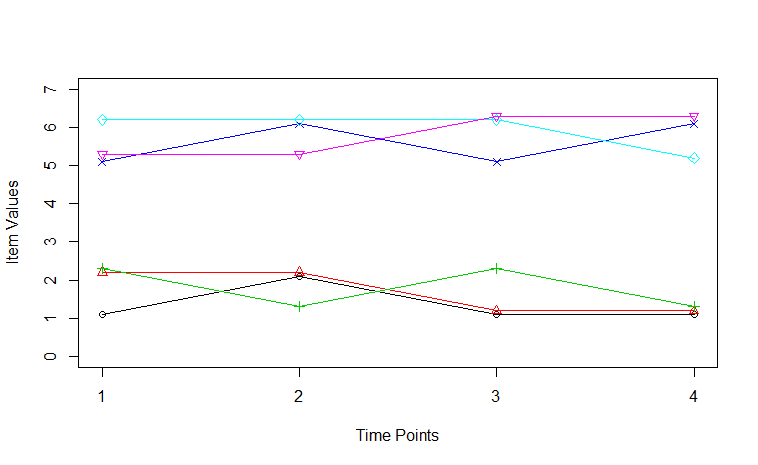
\includegraphics[width=0.75\textwidth]{images/chapter3/timeSeriesModel.png}}\\
		
		\subfigure[Focussing on the time points]{
			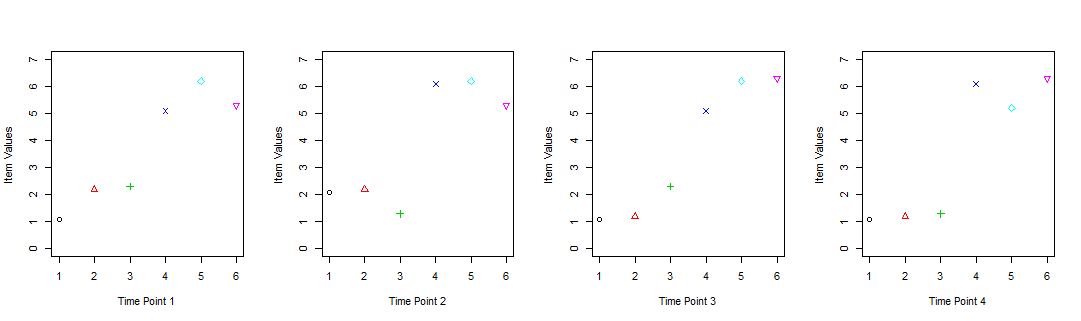
\includegraphics[width=.95\textwidth]{images/chapter3/timePointsModel.png}}
		\end{minipage}}
	\caption{Two different models focussing on temporal data. The first one focuses on the individual time series items while the second focuses on the time points and evaluates items according to their value in that time point. }
	\label{fig:temporaldatamodel}
\end{figure}

Before finding items' behavioural difference between any two time points, we had to find the categories for the behaviour of the items and how to group items according to these categories. It is important to categorise these behaviours so that neither nuance changes nor the shift of all groups are considered as a change in behaviour. For example, if we have two groups (poor and rich) of people's behaviour regards annual expenditure a slight change in the expenditure can not be considered as a significant change of behaviour, one that changes its status from poor to rich or vice versa. Moreover, a change of expenditure for the entire categories' might not be an indication of the change of behaviour. Instead, it may be due to inflation.

Another issue which could affect how to measure differences between time points in a data set with multiple time points (more than two time points) is what to consider as a normal reference behaviour of the item. By normal behaviour, we mean the general behaviour throughout in their data set. The first data point or any particular data points might not be a representative behaviour of an item. Therefore, this problem has also been addressed using different approaches in the study.


\section{Measuring Changes Over Time}
\label{MeasuringChangesOverTime}

As we mentioned in chapter two, the available methods for measuring changes over time focus on the overall changes in the clusters, agglomeration or the concentration of the of the data. These methods overlook the changes of the individual elements inside these clusters. In this section, we try to provide a method to quantify the magnitude of changes which reflect the change of items in a population. This is important to see the changes over time for individuals and the effect of an experiment. For example to measure the effectiveness of a new medicine or new teaching method can be quantified by measuring the change which individuals undergo in that process. In our case, it is required to measure the strategy change of players in public goods games which reflects the learning process that any player might undergo.

Measuring behaviour differences of items between time points requires three steps: The first step is to address time points, the second step is grouping similar behaviour and the last step is to find and measure the amount of differences between these time points. These steps will be addressed in the following paragraphs, and will be implemented and tested on the data in the next chapter.

The temporal data has to be split into separate time points. If the temporal data has discrete records of time, then each timestamp can represent a single time point. If the data set has continuous timestamps, then it might be converted to discrete using fixed intervals of time windows as used by many studies like \cite{Spiliopoulou2006}. It might be preferable that the time points have similar intervals between them so that the behavioural change measure M can represent the difference between any two time points in the same data set uniformly. Moreover, the items in each times point have to appear exactly once. This means if the items appear more than once in each time point an average value can be evaluated for the window. As an illustration consider $t \in T$ and the time intervals between [t-1, t] and [t, t+1] are equal which makes $m1 = \delta(t-1, t)$ and $m2 = \delta(t, t+1)$, so m1 and m2 can represent the two defined time intervals uniformly.

The second step is grouping similar behaviours of the items in the data so that we can identify each items' category of behaviour at every particular time points. As defined by Estivill-Castro \cite{Estivill-Castro2002} clustering is the task of finding groups of more homogenous (similar)members in a heterogeneous group of objects. Each time point is, thus, clustered using one of the clustering methods to find similarly behaving groups at each time point. The clustering algorithms used in the process of measuring the difference between time points in this study are K--means, PAM, and hierarchical clustering. Please refer to the previous chapter for the definitions and properties of these clustering methods.

Clustering items in each time point eliminate both the problems introduced in the previous section, namely potential minor changes in behaviour and the shift of all items in the same group. These problems are solved by clustering each time point separately without being influenced by other time points. Clustering will ensure that any values attributed by minor changes in items do not affect their membership in the group, and clustering each time point's data independently ensures that the entire movement of a group will not affect the measures of items' behaviour change. Please see Figure \ref{fig:lable1} for further illustration.

\begin{figure}[!h]
	\centering
	\subfigure[Original data set]{
		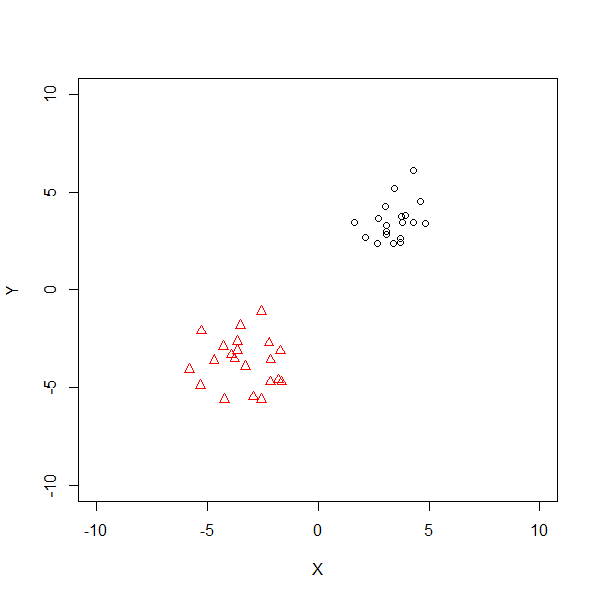
\includegraphics[width=0.32\textwidth]{images/chapter3/behaviourOriginal.png} \label{behaviourOriginal}
	} 
	\subfigure[Small behaviour changes]{
		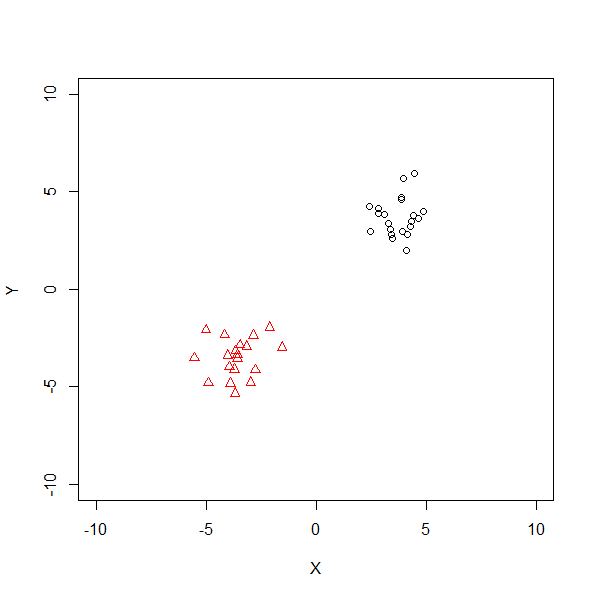
\includegraphics[width=0.32\textwidth]{images/chapter3/behaviourSmallChange.png}\label{behaviourSmallChange}
	}
	\subfigure[Entier group shift]{
		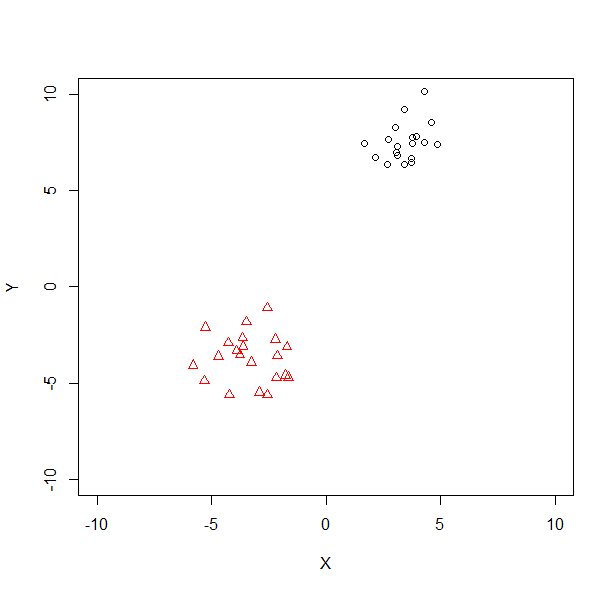
\includegraphics[width=0.32\textwidth]{images/chapter3/behaviourGroupMove.png}\label{behaviourGroupMove}
	}
	\caption{Three figures illustrating the small changes and the entire cluster move between two time points }
	\label{fig:lable1}
\end{figure}

The last step is to find the number of items which have changed their behaviour significantly so that they can be counted as they are in other groups or using the percentage of items' behaviour change. This means finding the $\delta$ function as described in the previous section. It is also possible to use AUC of ROC to find the difference between items' clusters in any two consequent time points by using cluster labels of t and t+1 instead of true class labels and predicted classes by a classification model as inputs to the AUC function so that it finds the difference between these two time points.

However, straightforward counting of items in clusters or using clustering labels as classes of the items might not be possible as it is hard to find one to one matching between clusters in consequent time points as described by Gunnemann et al. \cite{Gunnemann2011} and Xu et al. \cite{Xu2013}. Therefore, we use external cluster validity indices to compare between clusters of two time points and we replace the external labels with t cluster labels and guessed clusters by a clustering algorithm with t+1 cluster labels. This method can present a scalar measure as an indication of how much difference there exists between any two time points.

Multiple tests are implemented in Chapter four to check that this method can reflect the change in items' behaviour which is happening to the clusters (same behaviour grope). The tests include multiple external clustering indices as well as finding cluster pairs across time points so that other techniques like AUC can be tested. However to solve the problem of behaviour reference for the items as described in the previous section a new classification method is proposed. This will be elaborated on in the next section, and the detailed implementation of it in Chapter five.

 


\section{Temporal Rule-Based Classification}
\label{sec:Temporal-Rule-Based-Classification}
This section describes and explains the methodology for implementing the proposed rule-based temporal classification. As it has become obvious by now, this method targets temporal data with univariate or multivariate attributes. However, as stipulated by economists, the experts of public goods game, the rules should be presented in a simplified way, one human agents can understand. This provides simplicity and clarity with regards the rules for classification, and are expressed by using aggregated attributes which are derived from the temporal attributes. However, the final rules are formulated by considering of the temporal origin of these aggregated attributes.

\begin{figure}[!h]
	\centering
	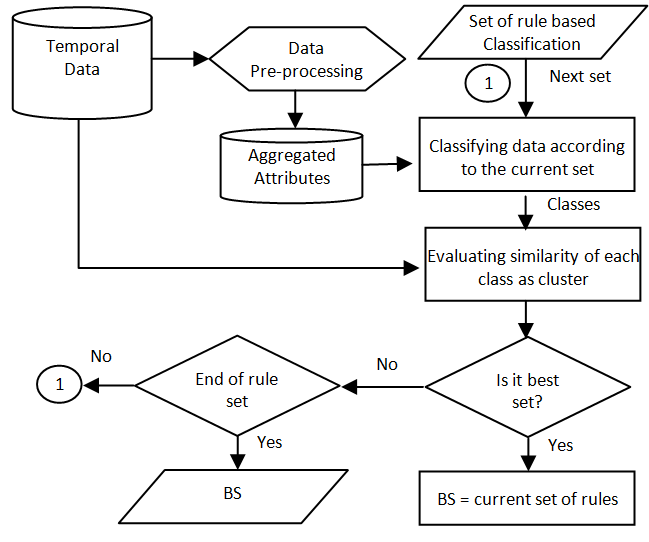
\includegraphics[width=0.7\textwidth]{images/chapter3/FlowchartTemporalClassification.png}
	\caption{The flowchart of the proposed rule-based temporal classification}
	\label{fig:FlowchartTemporalClassification}
\end{figure}

To achieve the conflicting goals of simplicity and consideration of the temporal attributes the classification process is divided into two main steps; rule generation and rule optimisation (as shown in the Figure \ref{fig:FlowchartTemporalClassification}). In the first step, rules are expressed using aggregated attributes of items with ranges of [min, max] values for each rule. In the second step, this range is optimised using temporal attributes to find the best cut in the provided range and select a single value for the rule.



This method might be both more effective and flexible than using aggregated attributes alone to classify items as it provides the flexibility to optimise rules in various ways: First, the aggregated attributes can be driven and optimised from different sets of items' temporal attributes. Second, it provides a way to include multiple inconsistent or overlapping ideas of experts on boundaries of classes, and by optimising these rules, the best possible classifier will be produced. This data set might be beneficial for cases when the items have both temporal and static data like expenditure behaviour (temporal) and career specialisation. Starting with a flexible model of rule-based classification and then determining the cut with an optimisation process might solve the problem of overfitting. This is because there is no requirement for the new data in the data set to follow the final cut of the old data, and the optimizer might generate slightly different values for final rules.


\subsection{Generating Initial Rules}
\label{sec:Generating-Initial-Rules}
Providing flexible rules for class boundaries is the first step of the temporal rule-based classification. To obtain these initial rules, this classification mainly relies on the experts of the field of knowledge for the data set and the intended items to be classified to obtain. As mentioned, the rules should be easy to read and interpret by human experts so that the provided rules are classifying temporal data sets on the basis of aggregated functions for each time series. However, the final result will also depend on the time dimension of the items.

There are numerous ways of using experts' knowledge to create classes boundaries to classify items. The most accessible method is to use their definition for the classes to create the rules for them. However, the definitions might not exist or can not be applied directly to the data. The second method involves asking their opinion on the rules of each class for the existing data. Experts' opinion can be developed interactively in multiple stages by creating profiles for items and viewing the results of previous rules that they have provided. Items' profiles illustrate their properties in a way that experts can create their opinion about the rules for the underlying data set.

To provide simple rules for classes so that they can be used by human agents to form definitions from them, complex temporal attributes have to be aggregated using one of the available functions such as the minimum value, maximum value, mean, mode, median and standard deviation. Each time series of the temporal data (items' specific data) can be aggregated using one or more of the aggregation functions so that sufficient quality and quantity of attributes are created to meet the requirements of the rules.

By flexible rules, we mean that each rule (or condition) has a range of candidate values which might fit it. The general form of the rule can be written as \textbf{$Attribute \left \{OP\right \} Value$}. The $Attribute$ can be any static property of the items either derived from a temporal attribute of the items using an aggregation function or other static values which are in the data set recorded separately from any temporal attribute. The $Value$ is a vector which contains all possible cuts between two classes. It can be expressed as [min, max] pairs to represent the beginning and the end of the range of the cut between two classes in its dimension. The $ \left \{OP\right \} $ can be any of the comparison operators like $\left \{\leqslant , \geqslant , < , > , = and \neq \right \}$. The classes might have multiple conditions which represent the boundaries of the class. These conditions can be combined using logical $and//or$ operators. Figure \ref{fig:illustrationofRules1} shows an illustration for ranges of values created by using flexible rules for two attributes to split items into different classes.

\begin{figure}[!h]
	\centering
	\includegraphics[scale=0.55]{images/chapter3/illustrationofRules1.png}
	\caption{An illustration of the ranges which splits between neighboring classes. These ranges will be changed into crisp lines after optimisation process}
	\label{fig:illustrationofRules1}
\end{figure}

The range value [min, max] of two neighbouring classes for the same attribute might overlap due to the differences in experts' opinions about each class limits or from slightly different definitions for each class. To prevent an item possibly falling into two classes at the same time due to the overlapping problem, the classes have to be prioritised. This means when an item fulfils the condition of the higher priority class, there is no need to check for lower priority classes. This might be done using a nested if-else statements. Moreover, the lowest priority class might be without any condition because if an item does not fall into any class category, they might be in the last one. However, if conditions are not used for the least priority class, a careful design for higher priority classes should be undertaken to prevent ambiguity or it might be better to consider a non-exclusive label for the last class like others or not-determined.


The next step focuses on changing the ranges of values of rules into single values by using temporal attributes of the items.



\subsection{Optimising Initial Rules}
\label{sec:Optimising-Initial-Rules}

The result of the first step of temporal rule-based classification is creating generalized rules with indeterminate boundaries of classes for classifying items. In the second stage, the boundaries of classes will be converted from vector ranges of values to scalers with a single value. Figures \ref{fig:illustrationofRules1} and \ref{fig:illustrationofRules2} should be compared to provide an illustration of the task for this step of classification. To link temporal features of the items and their corresponding non-temporal aggregate attributes, which are generated to create rules for classification, this stage will use temporal data to decide on choosing a scalar among the provided range of values. 


\begin{figure}[!h]
	\centering
	\includegraphics[scale=0.5]{images/chapter3/illustrationofRules2.png}
	\caption{An illustration for the boundaries of classes and how the ranges are converted into line separators.}
	\label{fig:illustrationofRules2}
\end{figure}


For each provided vector in the rules, this step finds the best scalar to divide adjacent classes. The point is considered as the best dividing point when it produces the most compacted classes of items at every time point using the temporal features to measure the distance between items. This process can be accomplished by iterating through all possibilities of the value ranges for the rule-based classifiers, as implemented in chapter five or using a heuristic search algorithm as implemented in chapter six using Differential Evolution. See algorithm \ref{alg:bruteForceOptimization} for the brute force method to determine the best classifier.

\begin{algorithm}[!h]
	\SetAlgoLined
	\KwData{Temporal data and aggregated attributes to represent classification rules}
	\KwData{R= set of classification rules which includes discrete value rages}
	\KwData{minCost = Inf}
	
	\ForEach{r in R}{%
		c = classify(PG, r)\;
		cost = calculateCost(c)\;
		\If{cost < minCost}{
			minCost = cost\;
			bestClassifier = r\;
		}
	}
	print bestClassifier\;
	
	\Fn{calculateCost (C)}{
		\ForEach{t in Periods}{%
			\ForEach{c in Classes}{%
				costs.append(CM(ct ) * count(c))\;
			}
		}
	}
	
	\caption{Using brute force to optimize rule ranges}
	\label{alg:bruteForceOptimization}
\end{algorithm}


The classification step uses provided rules with a single value for each range of the values. If the value ranges are continuous, they should be discretised into acceptable discrete values. Selecting the acceptable discretisation intervals is a specific area and underlying data which can be decided by consulting area specific experts. By iterating though all values, the classifier tries values to classify underlying data labels items accordingly and sends them to the next step to be evaluated.

The evaluation step uses item labels provided by the classifier of the previous step and uses temporal attributes to evaluate compactness of the classes in each time point. The compactness of classes can be calculated using different criteria, such as standard deviation, internal clustering indices or measures of distance. To calculate a measure for compactness, we created a weight function to be used as a cost function for evaluating the goodness of every classifier, and then returned the best classifier as a final result for the optimisation process. After this process, the items can be classified by the best rule-based classifier values.

For a generalised optimisation process, it can be assumed that experts' definitions and consultations produce N classes for items have to be classified using aggregated attributes of temporal data, producing D of possible classifiers of rule-based classification for different ranges of values for each class. Our task is to select the best classifier among a set S of size D classifiers, hence reducing each provided separator range between neighbouring classes into a single line of separation, using the temporal attributes of T time points. A cost function  for each $C \in S $ can be produced using any \acrfull{cm} that measures the goodness of classes in each time point. The can be defined as: 
\begin{equation*}
	f(C) = \sum_{t=1}^{T} \sum_{n=1}^{N} CM(c_{n}^{t}) \times \left | c_{n} \right |
\end{equation*}
where $ \left | c_{n} \right |$ is number of items in each class to prevent creating single big classes. The classifier with the smallest $f(C)$ value can be considered as the best classifier among S.

\subsubsection{Evolutionary Algorithms}

In nature, evolution consists of two steps, selection and random variation. A population of individuals living in an environment do not have the exact same traits. Some of these traits might be more advantageous and fit better for that specific environment. These individuals have more chance of surviving and producing offspring while others will die out. This fitness for the experiment is the natural selection. The surviving individuals will carry their traits through to the next offspring of the population though DNAs. However, the offspring of the surveyed individuals might not have the exact DNAs as their parents because the operation of replicating DNAs consists of randomly crossing both parents' DNAs. The operation itself might result in some errors which might lead to new mutations. This operation of creating new traits through random crossovers and mutations is called random variation which might be more beneficial (best fitting) for the environment
 \cite{Back1997}. 

Evolutionary Algorithms are inspired by the natural evolution in biology. Given that, they comprise the same steps as their natural counterfeits. There are many flavours of the algorithm with slightly different implementations. However, all of them have the same basic components as shown in shown in Figure \ref{fig:EALifeCycle}, this figure represents the general flowchart for evolutionary algorithms \cite{Eiben2015}.

\begin{figure}[!h]
	\centering
	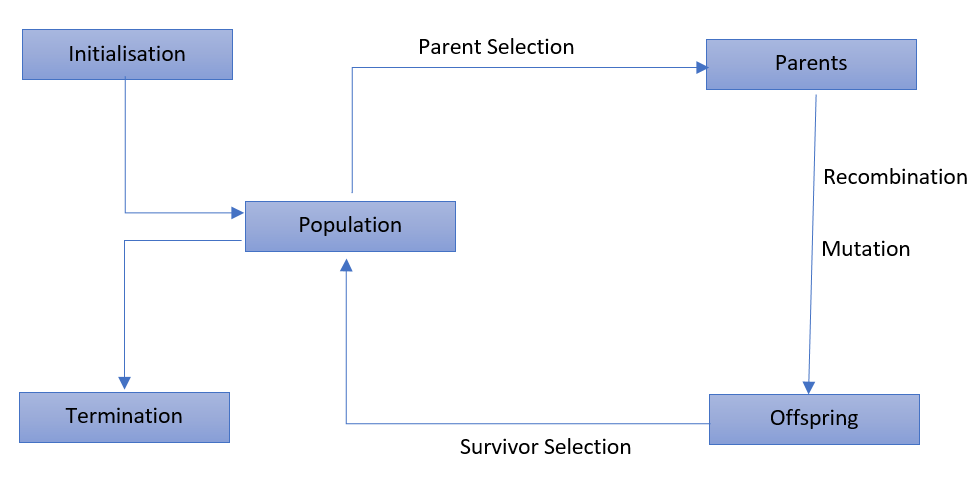
\includegraphics[scale=0.4]{resource/EALifeCycle}
	\caption{General operations of evolutionary algorithms. 
		From Eiben et al. \cite{Eiben2015}.}
	\label{fig:EALifeCycle}
\end{figure}

In their book \cite{Eiben2015} Eiben and Smith listed the components of evolutionary algorithms as follows: 
\begin{itemize}
	
	\item \textbf{Representation}: Is the operation of mapping the real world into the Evolutionary Algorithm world. This process consists of translating phenotypes into genotypes which are typically accomplished by the domain experts.
	
	\item \textbf{Fitness Function}: Also known as evaluation function, this function assigns a quality measure for each genotype helping the process of selecting the desired behaviours from the population. Hence this function acts as the environment for a population which favours certain phenotypes according to their genotype. The most fitted behaviours or phenotypes represent the solution for the underlying optimisation problem of the evolutionary algorithm.
	
	\item \textbf{Population}: The population consists of individuals carrying different genotypes. These genotypes represent a possible solution for the issue of optimisation. In most evolutionary algorithms, the population size remains constant, which means that after producing a number of the new generation, the same amount of the individuals will be eliminated for the next phase of the population.
	
	\item \textbf{Parent Selection}: Is a mechanism of selecting individuals to undergo the operation of generating a new individual (child). This process is statistical; this means, the individuals of a higher quality will be selected at a higher rate than low-quality individuals. Nevertheless, the low-quality individuals also have a high chance of being selected, so that the search does not become greedy and stuck in a local optimum.
	\item \textbf{Variation}: Variation consists of two different operations; recombination and mutation:
	\begin{itemize}
		\item \textbf{Mutation}: Is a stochastic process which changes some values of the selected children's' genotype to mimic the natural mutation. This process might produce individuals with better characteristics than the available population and helps to avoid local optima \cite{Grefenstette1986}.
		\item \textbf{Recombination}: Also called crossover, it is a process of creating the genotypes of new offspring using random parts of the selected parents' genotypes.
	\end{itemize}
	\item \textbf{Survivor}: Also called replacement, this is the process of selecting some new offsprings to survive and pass their genotypes to the next generation. This process, with parent selection is responsible for keeping the population size constant.
\end{itemize}



\subsubsection{Differential Evolution}

Differential Evolution is introduced by Storn et al. \cite{Storn1997} as a type of evolutionary algorithms. As described by Storn et al. \cite{Storn1997}, this method can optimise nonlinear, none-differentiable continuous and multidimensional space function.

The obvious difference between differential evolution and other evolutionary algorithms like genetic algorithms is it can operate on real numbers rather than integers. Furthermore, differential evolution employs the components of evolutionary algorithms in a different way as described below \cite{Storn1997}:

\begin{itemize}
	\item \textbf{Initialisation}: The initial population must cover the entire search space. This can be accomplished by randomly assigning values for the individuals. The random values have to be in the range of the minimum and maximum values of the search space.
	
	\item \textbf{Mutation}: Mutation is accomplished by creating a mutant vector from individuals of the population. This is called target vector. The mutant vector is a result of a target vector and the difference of two vectors which might be chosen randomly or from the best quality individuals.
	
	\item \textbf{Crossover}: Is the operation of copying a fraction of the mutant vector to its corresponding target vector. This ratio of the copy is constant and can be controlled by the end user. If the values of the resulting individual exceed the range of the search space, this individual will be reinitialized. 
	
	\item \textbf{Selection}: In this stage, the fitness value of the target vector and resulted vector will be compared. The best fitted vector will survive and the other one will be eliminated.
\end{itemize}


In chapter six of this study, we will use Differential Evolution with the proposed classification method to optimise a classifier from a pool of classifiers provided by domain experts. The reason behind choosing differential evolution for optimising the proposed classification method is its characteristics as described by Stor et al. \cite{Storn1997}. It has been successfully implemented with multiple data mining methods as listed by Das et al. \cite{Das2011}. Furthermore, Tusar et al. \cite{Tusar2007} proved that for most cases differential evolution is more efficient and effective than other genetic algorithms that use multiple benchmarks.


\section{Statistical Measures and Tests}

In this thesis, multiple statistical measures and tests are used for different reasons such as measuring the spread of a variable or finding similarities between resulting samples. In the following subsection, we briefly introduce some of these statistical tools. They are used across multiple chapters of the thesis. Other statistical measures, when used, will be introduced in their respective chapters.


\subsection{Variance and Standard Deviation}

Variance measures the spread of random variables around their mean. It uses the sum of squared difference between readings and the mean to calculate the amount of spread \cite{Kenney1947}. For the random variable $X$ which consists of $N$ readings and its average is $\overline{X}$ its variance ($\sigma^{2}$) will be:

\begin{equation*}
	\sigma^{2} = \frac{\sum (X - \overline{X})^{2}}{N -1}
\end{equation*}

\acrfull{stdiv} measures spread of variables as it is calculated as a square root of variance $\sigma^{2}$. It is denoted as $\sigma$. In this thesis, we refer to standard deviation as StDev. To calculate the standard deviation \cite{Kenney1947}:
\begin{equation*}
	\sigma = \sqrt{\sigma^{2}} = \sqrt{\frac{\sum (X - \overline{X})^{2}}{N -1}}
\end{equation*}


\subsection{Interquartile Range}

\acrfull{iqr}, also known as H-spread, is the range of the middle half of a random variable. For a ranked variable, the total range of the data is divided into four quarters that is Q1, Q2, Q3 and Q4. Each quartile consists of 25\% of the readings. The Interquartile Range can be calculated as $IQR = Q3 - Q3$ \cite{Ross2010}. This range can be considered as another measure of spread. However this IQR ignores the outliers and extreme readings of the variable.

Quartiles can be graphically represented as boxplots. Normally a boxplot has a vertical line representing the range of values of the readings in the variable with horizontal lines cutting through the main vertical line showing the range of each quartile. The second and third quartile are placed in a box demonstrating the IQR of the variable as shown in Figure \ref{fig:boxplotIllus}.

\begin{figure}[!h]
	\centering
	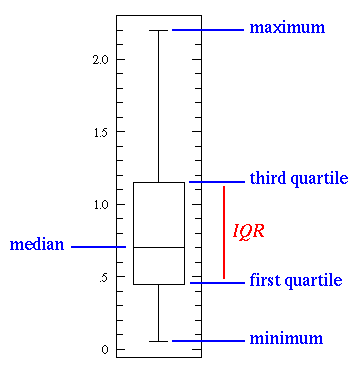
\includegraphics[scale=0.5]{images/chapter3/boxplots.png}
	\caption{An illustration of different parts of a boxplot showing quartiles and their interquartile range. From Kirkman \cite{Kirkman1996}}
	\label{fig:boxplotIllus}
\end{figure}

\subsection{Wilcoxon Test}

The Wilcoxon ranked test is a statistical method to test the null hypothesis of median equality between two paired variables \cite{MCDONALD2008}That is, the same sample has been used for two different experiments, in contrast to the t-test, this test does not assume normality of distribution for data which, thus, makes it a non-parametric test. However, it assumes that data is symmetric around median \cite{MCDONALD2008}. 

\subsection{Friedman Test}

The Friedman Test is a statistical non-parametric ranked test which can treat multiple dependent samples sets \cite{Ross2010}. The null hypothesis of the Friedman Test is that there is no difference between variables. The null hypothesis can not be rejected if the result of the treated testes is higher than the pre-appointed significance value \cite{Friedman1940}. Non-parametric means that this test does not assume normality in the sample (that is, the condition of using this test is the data require a normal distribution around the mean) \cite{Ross2010}.

This study uses the Friedman test to find the significance of the differences between the results of the proposed methods, and other available methods of classification and measuring changes over time. Given the characteristics of the Friedman test, multiple samples can be compared without assuming normality. Moreover, this test is used in data mining and data analysis to compare the results of different algorithms of classification \cite{Demsar2006} and methods of concept drift \cite{Goncalves2014}.


\section{Used Data Sets in This Study}
\label{section:Used-Data}

In this study, four data sets are used for different purposes. A synthetic data is used to evaluate the fitness of the external clustering validity to measure the differences in the data. Two data sets of the public goods game are used to measure the players' behaviour change over time and classify them using the proposed method. The final data set is that of a stock market, which is used to test whether the proposed methods can be generalised to other cases or not.



\subsection{Creating a Synthetic Data}
\label{CreatingaSyntheticData}

To check the validity of our method for quantifying behaviour changes of items over time, we create a simple 2D data set. These items are agglomerated to form four distinct clusters with their centres separated around the origin (0, 0) point. The original data set is mutated to create the next time point and to simulate the behaviour change of items.

We used the mlbench.2dnormals method of package mlbench of R language which is developed by F. Leisch and E. Dimitriadou \cite{mlbench210} to create the original data set\footnote{The R code for creating this synthetic data set is available at https://goo.gl/8DBuII}. The data set contains 500 (x, y) items (points) separated randomly among four clusters. Each cluster's centre is placed on a circle with a radius equal to 6, and its centre is point of origin (0, 0). Items inside each cluster have a Gaussian distribution and spread from its centre with 1.5 of standard deviation. Please refer to Figure \ref{fig:synthesisData_first} to see the produced data set and its items distribution among clusters.

To create the effect of time passing and items behaviour change, the set is mutated to create the next time point. By repeating the mutation process on the previously mutated data set, multiple time points are created (for our tests, 20 time points are created). For the data set DS for time t, D(t+1) = D(t)' where D(t)' is the mutated version of D(t). 

Two methods are used to mutate the data and generate the next time point. First, by changing the x and/or y coordinates sign value from positive to negative or vice versa of a randomly selected number of items. This change of sign make items jump from one cluster into another. The first change of data can be considered as a big change, which leads items to change their behaviour significantly. The second kind of change is introduced to all items in the data set by slightly changing their x and y values so that they will jiggle from their position without leaving the cluster. The amount of jiggle depends on the x and y values of the item as each item will be displaced with a random value range from 1\% to 2\% of its original value. Please refer to Figure \ref{fig:synthesisData_mid} and \ref{fig:synthesisData_last} for the mutated data sets which represent the middle and last time points for the temporal data set.

\begin{figure}[t]
\centering

\subfigure[First time point]{
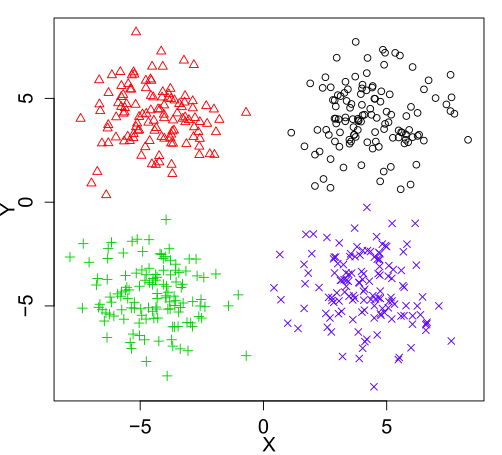
\includegraphics[width=0.31\textwidth]{images/chapter3/synthesisDataFirst.png}\label{fig:synthesisData_first}}
\subfigure[Middle time point]{
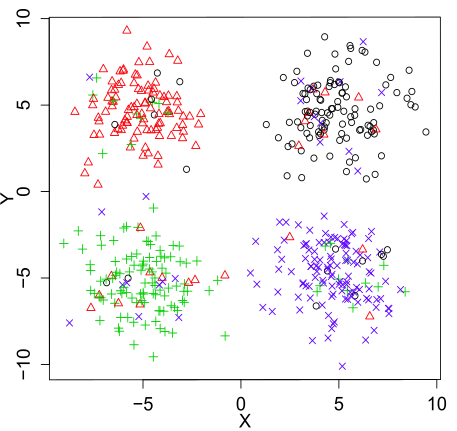
\includegraphics[width=0.30\textwidth]{images/chapter3/synthesisDataMid.png}\label{fig:synthesisData_mid}}
\subfigure[Last time point]{
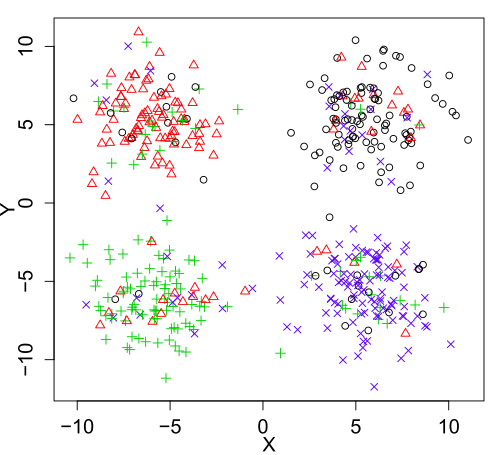
\includegraphics[width=0.30\textwidth]{images/chapter3/synthesisDataLast.png}\label{fig:synthesisData_last}}
\caption{Three time points (first, middle and last) from the overall created 20 time points. The first time point which contains 500 items separated into four clusters is the original data set other time points are created by mutating (jumping) items of four clusters from one cluster into another.}
\label{fig:synthesisData}
\end{figure}

\subsection{Public Goods Games Data}
\label{PublicGoodsGamesData}
There are many variations and set-ups for the public goods game experiment (cite), However, the data which has been used in this study is collected through experiments conducted by Fischbacher et al. \cite{Fischbacher2012}. Their experiment for public goods game consists of two sub-experiments; \gls{P-Experiment} and \gls{C-Experiment}, both of which every participant (player) has to accomplish. In the following sections, we will explain how these two sub-experiments are conducted, and then describe the collected data which will be used in later chapters.

\subsubsection{Game Set-up}

Prior to each sub-experiment of P-experiment and C-Experiment, experimenters explain the rules of the game for the participants so that they understand the rules, and how their decision will affect their result and the number of points available. Participants should answer a number of control questions correctly to demonstrate their comprehension of the game. Experimenters make every effort to ensure that the players are paying attention and playing thoughtfully by rewarding them extra points for correct guesses and well-thought out decisions during the game.

In P-experiment, four players start the game with 20 points each in their private account and they can contribute any amount they deem necessary to a project which represents public good. The amount which they do not contribute in the project will be kept only for the players themselves. The collected amount from the project will be distributed among all players regardless of their contribution to the project. The amount of points each player can accrue from the project is determined by this equation:

\begin{equation*}
Player Share From Project = Total Amount Of All Players Contribution * 0.4
\end{equation*}
So that each players total point after the game will be:
\begin{equation*}
Player's Points = (20 - Contribution In The Project) + Player Share From Project
\end{equation*}

In P-Experiment, players are asked to make two kind of contribution; conditional and unconditional. In conditional contribution, players are asked to decide what amount of points they wish to contribute in response to the rounded average of other players' contributions. This contribution will be filled out by the player in a form called the contribution table as shown in Figure \ref{fig:pgg1RoundOfGame}. The unconditional contribution players will input the amount of contributions which they require in a single field without any conditions. Please see Figure \ref{fig:pgg20Questions} for unconditional contribution.

\begin{figure}[!h]
	\centering
	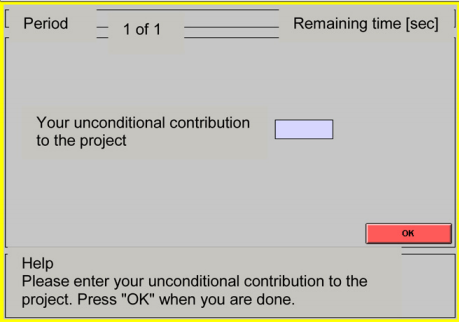
\includegraphics[scale=0.55]{images/chapter3/pgg1RoundOfGame.png}
	\caption{P-experiment's unconditional contributions user interface. which the user can enter their amount of contribution.
		From Fischbacher et al. \cite{Fischbacher2012}}
	\label{fig:pgg1RoundOfGame}
\end{figure}
\begin{figure}[!h]
	\centering
	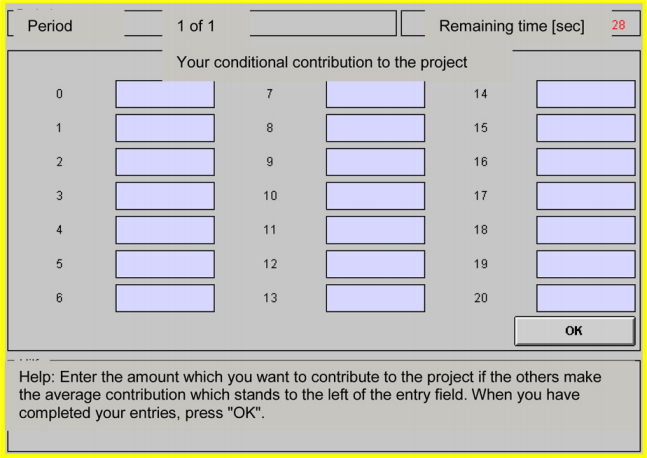
\includegraphics[scale=0.45]{images/chapter3/pgg20Questions.png}
	\caption{P-experiment Contribution table user interface in which the user can enter their contribution for all possible conditions. 
		From Fischbacher et al. \cite{Fischbacher2012}}
	\label{fig:pgg20Questions}
\end{figure}

For each player, only one of the two contributions will be selected by the computer as their final contribution to the project. One of the four players' conditional contribution will be randomly chosen to be used as their final contribution. while for the other three players their unconditional contribution will be used. This random selection of players' contributions is one of the mechanisms that experimenters have used to make sure that players are thinking thoroughly about their decision for the contribution to the project.

When the P-experiment is completed, players start C-experiment. C-experiment is similar to a repeated sequence of unconditional contribution except

this time the player, in addition to their own contribution, will be asked to guess other players' rounded average of contribution. After each round of the game, players will be notified of their total points in that particular game. The sequence length of the games can vary from one experiment to another. In this study, we will use data sets with 10 and 27 series of rounds of the game. In each round, four different random players will play the game so that players can not predict others' contributions in advance. Players will gain extra points if they make correct guesses about other players' rounded contributions. They will, therefore, not fill in the boxes
 randomly. Please refer to Figure \ref{fig:pgg10RoundOfGame} for the interface of C-experiment.

\begin{figure}[!h]
	\centering
	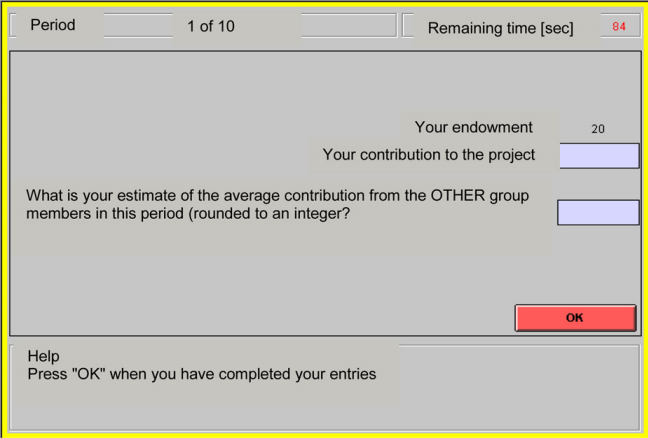
\includegraphics[scale=0.45]{images/chapter3/pgg10RoundOfGame.png}
	\caption{C-experiment user interface has two fields. One for the amount of players own contribution and the other for guessing other players rounded average contribution. From Fischbacher et al. \cite{Fischbacher2012}}
	\label{fig:pgg10RoundOfGame}
\end{figure}

\subsubsection{Data Set Attributes}

To measure and classify the behaviour of players in public goods games, this study used two different data sets. These experiments are conducted on different samples of players, so the first data set has 140 players and the second data set 128 players. These data sets have the same attributes and follow exactly the same experiment procedures, except for the P-experiment length, as the first one consists of 10 rounds while the other has 27 rounds.

Due to the limitations in space and equipment, all players in these experiments did not play at the same time. Instead they were distributed into multiple sessions. However, each session consisted of sufficient number of players meaning that the random selection of each four players playing with each other is unbiased. The behaviour of each player will not be affected by the session which they are in, as they are experiencing the game for for the first time and develop their understanding of the different strategies during P-experiment. Therefore, we are able to consider that the experiment has been conducted in one big session with all players playing the rounds of the P-experiment at the same time. This means for the first data set, we consider that all 140 players have played the first round of P-experiment at the same time.

The attributes of the data sets can be divided into two types the temporal and non-temporal attributes. The temporal attributes are generated in the P-experiment as it contains multiple rounds and non-temporal attributes are generated in C-experiment. The following is the list of all the attributes of the data sets. Please notice that the temporal attributes are underlined:
\begin{itemize}
\item \textbf{Idtyp}: labels for players categories assigned by experts. The categories are: conditional contributors = 1, free riders = 2, triangle contributors = 3, and others = 4. These categories are generated depending entirely on the b0-b20 attributes. Figure \ref{fig:percentage} shows the average contribution behaviour of players in each category. Please refer to the previous chapter for the detailed description of these categories.

\item \textbf{Idsubj}: a unique identifier for each player during both C and P experiments.

\item \textbf{b0-b20}: twenty one attributes representing the contribution table for each player as their response in C-experiment to every possible rounded average of other players' contribution.

\item \textbf{u}: the unconditional contribution of the player for C-experiment during the actual game.

\item \textbf{\underline{Predictedcontribution}}: Players' prediction about other co-players rounded average of contribution to the project.

\item \textbf{Period}: the session number for P-experiment. As P-experiment for each player consists of multiple rounds, each players' playing times are recorded to keep track of the number of games played.

\item \textbf{\underline{Contribution}}: players' actual contribution to the project in each round of the P-experiment.

\item \textbf{\underline{Belief}}: players' beliefs about other players average contribution in each session.

\item \textbf{\underline{Otherscontrib}}: Other co-players' rounded average contribution.


\end{itemize}

\begin{figure}[!h]
	\centering
	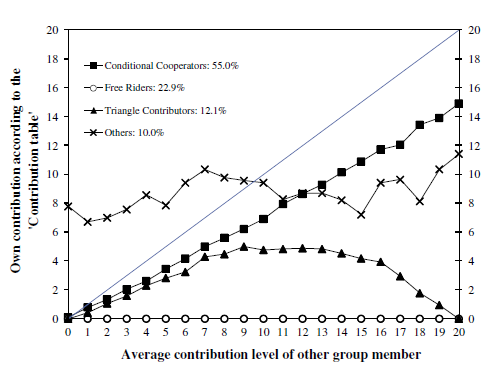
\includegraphics[scale=0.45]{images/chapter3/percentage.png}
	\caption{Four type of players average own contribution according to co-players average contribution }
	\label{fig:percentage}
\end{figure}

\subsubsection{Preliminary Behaviour Analysis of the Players}

As mentioned before, experts use C-experiment data to classify players' strategies. However, we are using the P-experiment data to classify players' behaviour over time and measure their overall change in contribution. So before starting the analysis for classification, it is beneficial to see the general trend of players' behaviour over time and gain an overall idea about them. Heat maps are used to identify the density of players' contribution at each round of the game with regards their beliefs about other co-players' contribution. The heat map shows the percentage of players who have the same contribution and belief. The more similar the behaviour is of the players, the darker the box of that value becomes. 


Figures \ref{fig:contribution1}, \ref{fig:contribution2} and \ref{fig:contribution3} represent players contribution-belief heat maps generated for the first, mid and last rounds of the first data set. As can be noticed, the overall players' contribution for the project and their belief of co-players contribution drop significantly from the first to the last round. However, it can also be noticed that the players contribution drops faster than their belief as more dark boxes can be seen at the bottom of Figure \ref{fig:contribution2}. This indicates players are starting to contribute less than what they believe the other players will contribute to the project to obtain more points from the project than contributing in it.

\begin{figure}[!h]
	\centering
	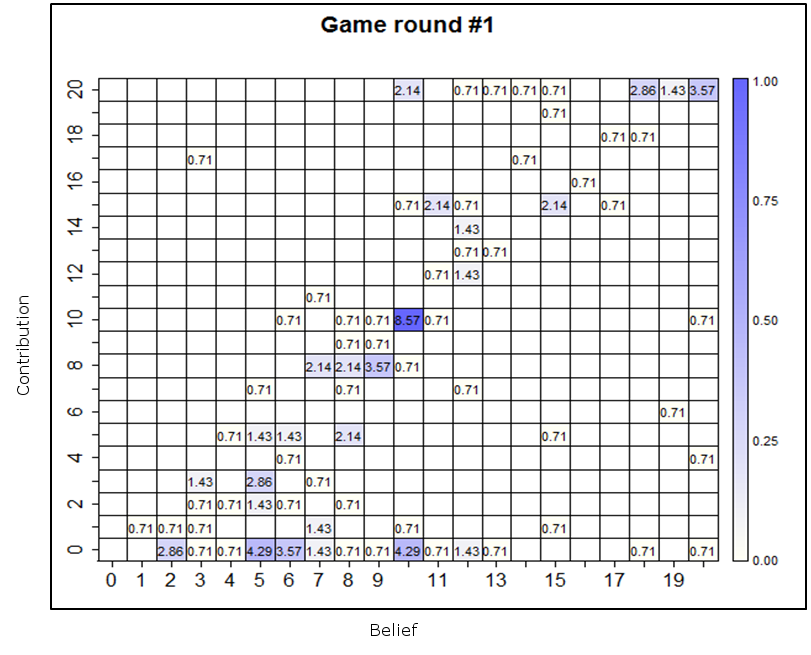
\includegraphics[scale=0.35]{images/chapter3/HeatMapContribution1.png}
	\caption{Heat map for players contribution according to their belief in round 1}
	\label{fig:contribution1}
\end{figure}
\begin{figure}[!h]
	\centering
	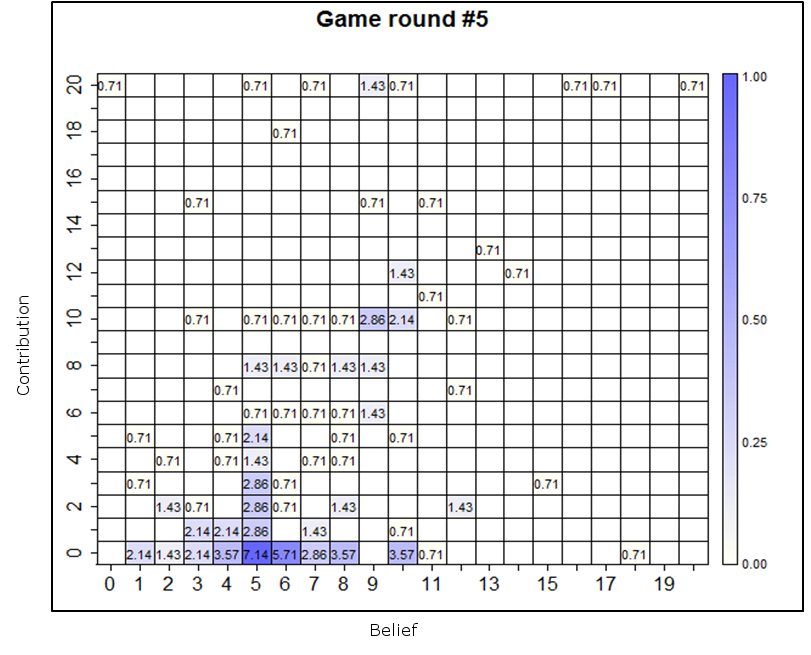
\includegraphics[scale=0.35]{images/chapter3/HeatMapContribution5.png}
	\caption{Heat map for players contribution according to their belief in round 5}
	\label{fig:contribution2}
\end{figure}
\begin{figure}[!h]
	\centering
	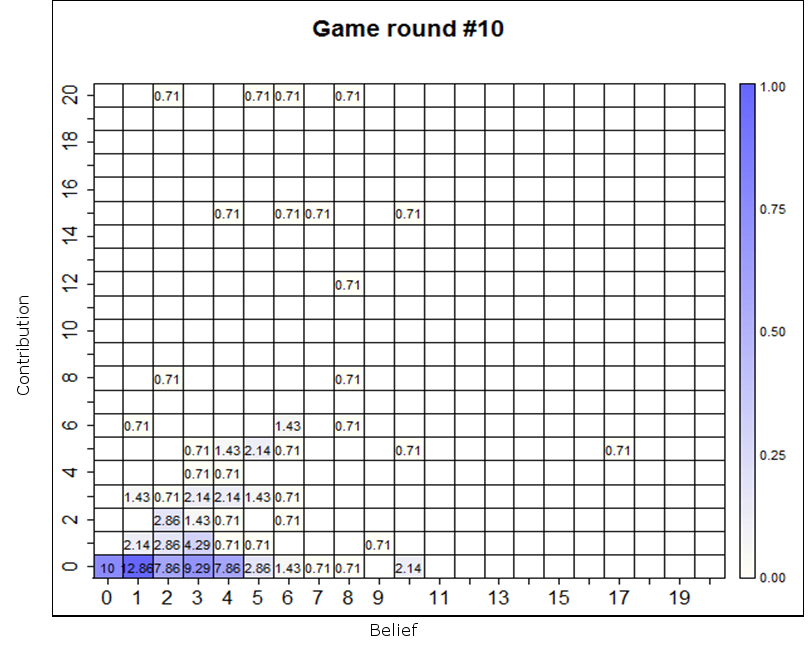
\includegraphics[scale=0.35]{images/chapter3/HeatMapContribution10.png}
	\caption{Heat map for players contribution according to their belief in round 10}
	\label{fig:contribution3}
\end{figure}

\begin{figure}[!h]
	\hfill{\begin{minipage}{\dimexpr \textwidth-2\fboxsep-2\fboxrule}% maximum allowed
			\centering
			\subfigure{
				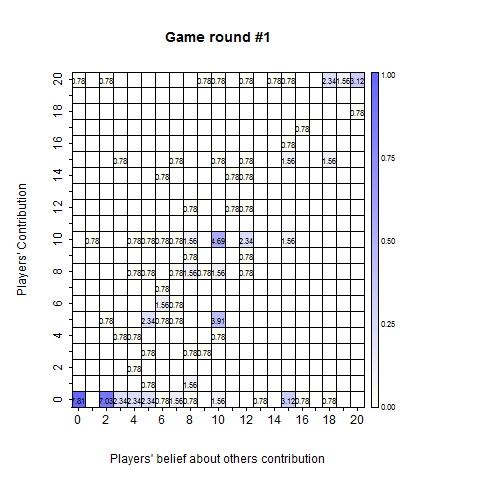
\includegraphics[width=0.45\textwidth]{images/chapter4/heatMap27/heatMap27_1.png}
			}
			\subfigure{
				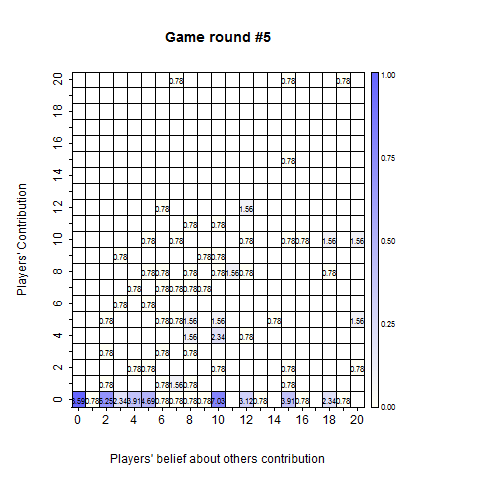
\includegraphics[width=0.45\textwidth]{images/chapter4/heatMap27/heatMap27_5.png}
			}\\
			\subfigure{
				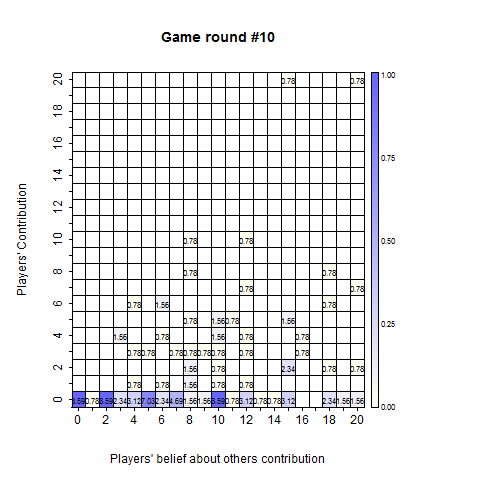
\includegraphics[width=0.45\textwidth]{images/chapter4/heatMap27/heatMap27_10.png}
			}
			\subfigure{
				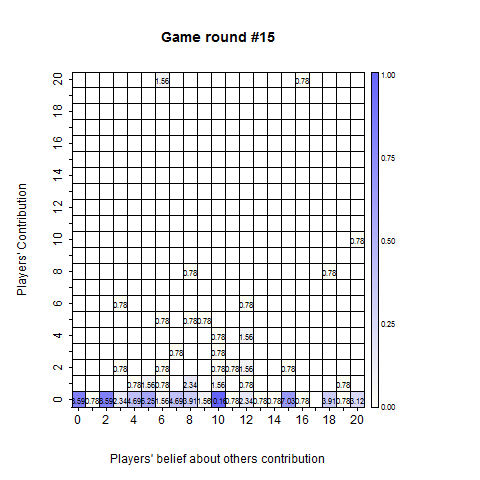
\includegraphics[width=0.45\textwidth]{images/chapter4/heatMap27/heatMap27_15.png}
			}\\
			\subfigure{
				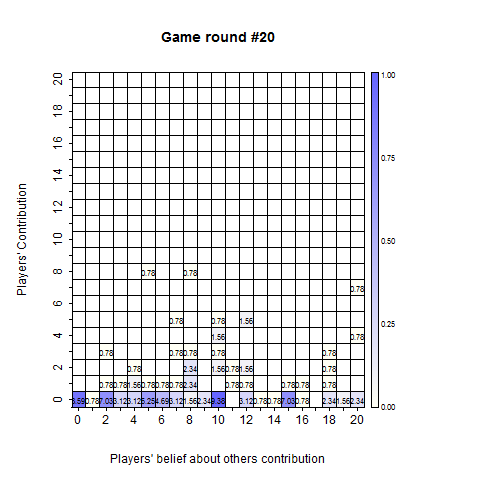
\includegraphics[width=0.45\textwidth]{images/chapter4/heatMap27/heatMap27_20.png}
			}
			\subfigure{
				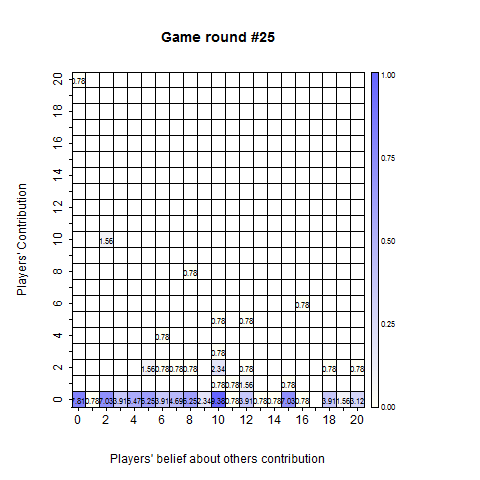
\includegraphics[width=0.45\textwidth]{images/chapter4/heatMap27/heatMap27_25.png}
			}\\
			
		\end{minipage}}
		\caption{Selected heat maps for players contribution according to their belief in rounds 1, 5, 10, 15, 20 and 25 in the 27 rounds data set}
		\label{fig:contributionRound27}
	\end{figure}

\subsection{Stock Market Data}
 We further tested the proposed classification and measuring methods using different data sets with similar required properties. The stock market data set was chosen as it contains elements (stock) in a temporal data with varying behaviour (prices). One advantage of the stock market data set is that we can select a larger set of unique items to be classified and longer time points to observe their behaviour change. This might be a good way to test the proposed methods to their full extent. However, the downside of the collected stock market data is that there are no pre-classified labels for the items in the data to be able to compare with in our findings. Therefore, we should rely on some other measures to evaluate our results.

\subsubsection{Data Harvesting}

For this study, we have selected \acrfull{sp500} stock market to run our tests as they contain a sufficient amount of items at each time point (502 items \cite{Goings2014}). In addition, it is publicly listed and this enables us to harvest long periods of their data freely. S\&P\,500, or historically known as Composite Index \cite{TheEditorsofEncyclopædiaBritannica} is designed to represent the large cap for domestic companies in United States \cite{Britannica2015}. This index comprises very diverse stocks which can be considered as a better representation of the U.S. market than Dow Jones . The large cap, in this context, refers to companies with more than 10 billion dollars worth of stocks \cite{Editors2016}.

We used the available symbols for the companies listed in S\&P\,500 index from \href{http://www.cboe.com/products/snp500.aspx}{cobe} website as it is specialised in market analysis. Symbol (or ticker) is a standard representation for a company in the stock market. We have used the list of S\&P\,500 symbols to download historic data of the companies from \href{https://uk.finance.yahoo.com/}{Yahoo Finance} website using an R script \footnote{The Symbols list, R script for fetching the data and manipulating it, and a sample of the data are available at \href{https://goo.gl/U0STqJ}{https://goo.gl/U0STqJ}}.

A sample data for all companies listed in S\&P\,500's index from 1-1-2015 to 1-7-2015, which represents a half year, are collected from the Yahoo finance website. The number of time points which are collected for this time period is 125 days, and the attributes for the collected data are:

\begin{itemize}
	\item \textbf{Date}: The date of the stock price. Each date can be considered as a time point and converted to a sequence of integer numbers.
	\item \textbf{Symbol}: The standard symbol which identifies companies' stocks.
	\item \textbf{Open}: The price of the stock at the opening time for that date.
	\item \textbf{High}: The highest price that the stock reached on that date.
	\item \textbf{Low}: The lowest price that the stock hit at that date.
	\item \textbf{Close}: The price of the stock at the close time of stock market at that date.
	\item \textbf{Volume}: The number of shares which are traded at that date.
	\item \textbf{Adj.Close}: The closing price of each stock might be amended to that date because of one of multiple reasons that might affect the price such as Stock Splits, dividends and Rights Offerings \cite{EditorsInvestopedia2016}. 
\end{itemize}

\subsubsection{Data Preprocessing}

The harvested data should be cleaned and pre-processed before using it to test the proposed methods. The unknown fields should be handled properly so that they do not subsequently affect the algorithms. The unknown fields are not the only problem as the stock price values from one company to another varies significantly. As this may affect the classification process, they should be normalised. Moreover, for the sake of simplifying the classification rules later, it is advisable to convert normalized data into integers. Table \ref{tab:stockdata} shows a sample of the data with its headers after the pre-processing stage.

\begin{table}[!h]
	\centering
	\caption{A sample of the S\&P\,500 data set after cleaning and manipulation.}
	\label{tab:stockdata}
	\begin{tabular}{|c|c|c|c|c|c|c|c|}
		\hline
		\textbf{Date} & \textbf{Open} & \textbf{High} & \textbf{Low} & \textbf{Close} & \textbf{Vol} & \textbf{Adj.Cls} & \textbf{Symbol} \\ \hline
		1    & 587   & 567   & 489   & 482   & 73    & 473    & A    \\ \hline
		2    & 440   & 406   & 367   & 351   & 137    & 344    & A    \\ \hline
		3    & 352   & 322   & 243   & 243   & 141    & 239    & A    \\ \hline
		4    & 303   & 282   & 292   & 333   & 300    & 327    & A    \\ \hline
		5    & 426   & 504   & 454   & 539   & 146    & 529    & A    \\ \hline
		6    & 556   & 508   & 474   & 487   & 87    & 479    & A    \\ \hline
		7    & 489   & 455   & 412   & 404   & 227    & 397    & A    \\ \hline
	\end{tabular}
\end{table}


A small number of the companies does not have the complete list of values for the specified date range on the Yahoo Finance website. As the proposed algorithm, cannot handle unknown data, they have to be handled prior to their use in the algorithms. One solution could be removing them from the data series so that we have different lengths of data series. However, this is not an option because we cannot properly study their behaviour for the full length. The second solution might be filling them with the average price from the available days prices. However, this will not reflect the proper behaviour of the stock. Therefore, we decided to remove these companies from the list as there is a limited number of them. The remaining symbols (companies) in the final list after removal is 497 companies.

We have converted dates into integers of absolute time points as the exact dates are irrelevant. Not all dates exist as there are stock prices only for working days in the week, and the proposed classification and analysis are concerned with the flow of consequent time points. Thus, the dates are ordered and each corresponding date is converted to an integer from 1 to 125. In this way, we preserve the correct sequence of the time points and simplify dates to a series of integers.

As the share price for companies varies, the effect of the same change in the price might have impacts on them. To eliminate the effect of this difference in share price, the data is normalised. The variables of each share price are normalized separately so that they scale from 0 to 1. For any variable (Close price, Open price, etc.) of share price x the equation of normalisation is used.

\begin{equation}
	{x}' = \left \lfloor \frac{x - min(x)}{max(x) - min(x)} \times 1000 \right \rfloor
\end{equation} 

The normalisation results for the shares are real numbers. To convert these numbers into integer numbers without losing their precision, each value is multiplied by 1000 and then its floor value is computed. As mentioned beforehand, converting price values to integer simplifies their analysis and classification rules. Moreover, by using integer values, we can compare the performance of the proposed algorithms between all available data sets.

\section{Testing Environment}

The machine used for carrying out the tests is a ThinkPad laptop with these properties:
\begin{itemize}
	\item Processor: Intel(R) Core(TM) i3-4000M CPU @ 2.40 GHz 2.40 GHz
	\item RAM: 8 GB
	\item System type: 64 bit Windows OS
	\item Storge: 100 GB of SSD
\end{itemize}

We used R language version 3.2.4 with IDE software RStudio V 0.99.893. The packages utilised for the R language is listed in Table \ref{tab:RenvirontmentPackages}.

\begin{table}[!h]
	\ra{1.3}
	\small
	\centering
	\begin{tabular}{lllp{6cm}}
		\toprule
		package & version & authors        & Usage                    \\ \midrule
		clv  & 0.3.2.1 & Nieweglowski \cite{Nieweglowski2013} & For validating clusters. Specially internal and external validity indeces methods \\ 
		DEoptim & 2.2.3 & Ardia et al \cite{Ardia2015}   & For differential evolution optimisation           \\
		dplyr  & 0.4.3 & Wickham et al \cite{Wickham2015}  & For data manipulation     \\ 
		dtw  & 1.18.1 & Giorgino \cite{Giorgino2009}   & For dynamic time wrapping algorithm \\
		gplots & 3.0.1 & Warnes et al \cite{Warnes2016}  & To create Heat maps        \\
		Hmisc  & 3.17.4 & Harrell JR \cite{Jr2016}    &                     \\
		mcclust & 1.0  & Fritsch \cite{Fritsch2012}   & For multiple clustering algorithms   \\
		mlbench & 2.1.1 & Leisch \cite{mlbench210}    & To generate data for tests   \\
		pROC  & 1.8  & Robin et al \cite{Robin2014}   & For classification evaluation specially AUC or ROC\\
		stargazer & 5.2  & Hlavac \cite{Hlavac2015}    & To create latex tables directly from R results         \\
		\bottomrule
	\end{tabular}
	\caption{The R packages which are used in this study}
	\label{tab:RenvirontmentPackages}
\end{table}

We also used Java programming \(JRE 8 update 92, JDK 1.8.0_92\) with Eclipse ''Marse.2'' IDE Version 4.5.2 to compare our results of measuring items behaviour change over time points with MONIC \cite{Spiliopoulou2006} results.


 

\chapter{Measuring Items' Behavioural Change}
\label{Chap:Measuring}

 
 \section{Introduction}
 
 This chapter addresses the research questions raised in chapter one regarding the use of clustering and cluster validity indices as a method to measure items behaviour through multiple time points. The questions and hypothesis will be tested using the methods mentioned in Chapter three Section \ref{MeasuringChangesOverTime} and related to items' behaviour measurement in temporal data.
 
 The Hypothesis \ref{hypo:diffCluster} in chapter one indicates that the result of quantifying the behavioural change will not be affected by using various clustering algorithms as long as all time points are clustered using the same algorithm. To test this hypothesis, we use multiple clustering algorithms like k--means, c--means, PAM and hierarchical clustering in this chapter to cluster the temporal data. Each clustering algorithm is used to cluster all time points of the temporal data set separately from each other and without the effect of the time attribute.
 
 Hypothesis \ref{hypo:diffCVI} indicates that different external cluster validity indices will produce similar results in measuring items' behavioural change between the various time points. To check the validity of this hypothesis, we used different external cluster validity indices to measure changes between any two time points. However, not all external cluster validity indices might be suitable to be utilised for this task as we, later in this chapter, will explain the essential characteristics of the measure which can be used. Moreover, we have used Area Under the Curve AUC of ROC analysis to measure changes over time for comparison purposes with external cluster validity indices.
 
 This chapter also partially addresses the reference of behaviour for items in temporal data (Hypothesis \ref{hypo:overallBehavoiur}). Reference of behaviour can be defined as a typical collective behaviour of elements of a temporal data set. Reference of behaviour can be used to compare other time point behaviours of items. In this chapter, we will use and test two different Reference of behaviours for items. However, after we introduce the proposed temporal classification method in the next chapter, we will use it to classify items in the data sets and use these classes as a reference of behaviour for all time points.
 
 Three data sets are used in our tests one synthetic data set to check the feasibility of using the proposed method as a measure of quantifying change over time and two different public goods games PGG data sets (as mentioned in chapter three, section  \ref{PublicGoodsGamesData}). Moreover, this chapter participates in the argument of the players' strategy change during the PGG rounds \cite{Chaudhuri2010, Fischbacher2009} by presenting a quantifiable method to measure the change in strategy by players.
 
 
 Finally, the results are compared with the MONIC model as it developed by Spiliopoulou et al. \cite{Spiliopoulou2006} to measure the cluster changes in the data streams (Further details on the MONIC method are provided in chapter two). The appropriate statistical analysis is presented to provide evidence supporting or rejecting the hypotheses of the first chapter.
 
 \section{Background}
 In economics, there is an interest in how players of public goods game change their strategy during multiple rounds of the game and jump from one strategy to another \cite{Fischbacher2010}, such as changing from conditional cooperator to free rider behaviour. This change can be seen as a drift from the original label assigned to the players.
 
 There are many methods for classification in machine learning, with the existence of concept drift \cite{Elwell2011,Garnett2008,Xiaofeng2014} and methods to detect it \cite{Baena-Garcia2006,Harel2014}. Moreover, measuring changes in clusters for different time points have been thoroughly studied in data analysis, especially for data streams \cite{Ntoutsi2011,Spiliopoulou2013,Yang2011}. However, these methods aim to find overall patterns of change in clusters' location, size, merging, emerging and/or dissipating rather than presenting a measure of how much change has occurred in each cluster (that is, in which ratio items change their membership from one cluster into another).
 
 External cluster validity is primarily used to check the performance of clustering algorithms by measuring the difference between ground truth labels given to the items by experts and the group in which they have been placed by a clustering algorithm \cite{Halkidi2002a}. This study uses external cluster validity measures such as variation of information \cite{Meila2003} VI and area under the curve of the receiver operating characteristic AUC \cite{Bradley1997} as scaler measures, to show the magnitude of items that jumped from one cluster to another between two consequent time points. To accomplish this measurement the items should be clustered separately in every time point. As the clustering is performed at a single time point, which eliminates the time dimension for the collected data on items, any traditional (non-temporal) clustering algorithm should theoretically be sufficient. After clustering, an external clustering validity measure can quantify the amount of changes between clusters at any two time points.
 
 
 \section{Approach}
 As has been explained in the previous chapter, to be able to measure the difference in behaviour of a population of items from their collected characteristics in a temporal data, the items should be clustered in each time point. Then their change in behaviour can be measured using cluster validity indices CVI or Aria Under the Curve AUC of ROC analysis. However, to implement the available methodology on a specific data, certain decisions have to be made to ensure that appropriate treatments are applied to the underlying data. In the following sub-sections, the rationale and reasons for selecting data set attributes, choosing the number of clusters, clustering algorithms and various cluster validity indices is explained.
 
 
 \subsection{Preparing Data Sets for Clustering}
 Before starting with clustering, the temporal data sets have to be separated by their time points. In this chapter, three data sets are used for the tests. The first data set is the synthetic data set as mentioned in section \ref{CreatingaSyntheticData}. The second and third data sets are public goods game data sets with different players and various length of time points.
 
 The synthetic data set is straight forward as it has 20 time points. So, the data will be split into 20 separate data sets with each subset representing one time point. The subsets are labelled so that the order of consequent subsets are preserved. The data has two temporal attributes in each sub-data set representing x and y coordinates.
 
 The first public goods game data set has 10 time points as presented by the ''period'' attribute so that it will be split into 10 subsets of data sets with each containing 140 items as the number of players in this data set. The second data set contains records of 27 rounds for 128 players so that this data set will be split into 27 subsets with each containing information of 128 players at a particular time point (round of the game).
 
 Both public goods game data sets have multiple static attributes and do not contain any temporal information. These static attributes are Idsubj, b0 to b20, u and Predictedcontribution. The temporal attributes are contribution, belief and otherscontrib. However, the otherscontrib is not directly related to the players' behaviour. Thus it is also not used in the clusterings. The only two attributes used are players contribution and belief of P-Experiment as these two attributes reflect the players learning the process for the game and the change in their ideas and strategies as the game progresses through rounds.
 
 \subsection{Choosing Clustering Algorithms}
 \label{sec:ChoosingClusteringAlgorithms}
 As each of the produced subsets of data represents one time point of the temporal data set, each subset alone, therefore, does not carry any information about the time dimension. This means it is possible to use non-temporal clustering algorithms to cluster items in each subset of the temporal data sets.
 
 
 Clustering algorithms can be categorised according to their method of finding similarities between items in the data. These categories are partitional, hierarchical, density-based, grid-based and fuzzy clustering \cite{Halkidi2001}. However, the main clustering categories which we used are partition based clustering,  hierarchical clustering and fuzzy algorithms. For the tests in this chapter, we used k--means and PAM as methods of partitioning clustering, hierarchical clustering with Euclidean distance and c--means as fuzzy clustering. As we aim to find similarities between items according to their distance from each other, we, therefore, did not use density-based and grid-based clustering methods.  Please refer to chapter two for further details on these clustering algorithms.
 
To find similarities between items, clustering methods can use linear distance measures such as Euclidean distance or use non-linear kernels to cluster complicated patterns in the data items. In the tests, we only used linear distance-based clustering methods because the aim was to find the similarity in behaviour based on the overall proximity of the attribute values of items. For the same reason, we did not use density-based clusterings such as DBSCAN and grid-based clustering such as STING since these methods do not depend on the mutual proximity of cluster items to a centroid. This represents a behaviour category.
 
 \subsection{Choosing Number of Clusters}
 \label{sec:Choosing-Number-of-Clusters}
 Most of the clustering algorithms require the number of clusters as an apriori condition to cluster the underlying data. This might be a challenging task especially for the data sets as there are no known patterns to start with \cite{Jain2010a}. Economists have classified players of public goods game data sets used in this chapter into four classes \cite{Fischbacher2001}. However, as explained in chapter three, these classes are dependent on the static attributes of the data rather than temporal attributes.
 
 Numerous methods exist to estimate the appropriate number of clusters in the data \cite{Milligan1985, Yu2014}. We used the elbow method \cite{Ketchen} to determine the number of clusters in the temporal attributes of the PGG data sets. This method involves clustering the data set repeatedly with an incremental number of clusters and then calculating the sum of square error or variance of items within clusters. By plotting the produced values, an appropriate number of clusters for the underlying data can be found.
 
 We used the ten round game data set to find the number of clusters in the temporal attributes of the public goods game data. The data is split into ten subsets with each subset representing one time point. Each time point is clustered repeatedly using k--means clustering, starting with 2 clusters up to 15 clusters. The sum of square errors within each cluster is calculated and plotted. The results in Figure \ref{fig:elbowNumberOfClusters} indicates that there is no absolute number for clustering. However, four clusters might be an accepted number of clusters for the data. 
 
 \begin{figure}[!h]
     \hfill{\begin{minipage}{\dimexpr \textwidth-2\fboxsep-2\fboxrule}% maximum allowed
             \centering
             \subfigure{
                 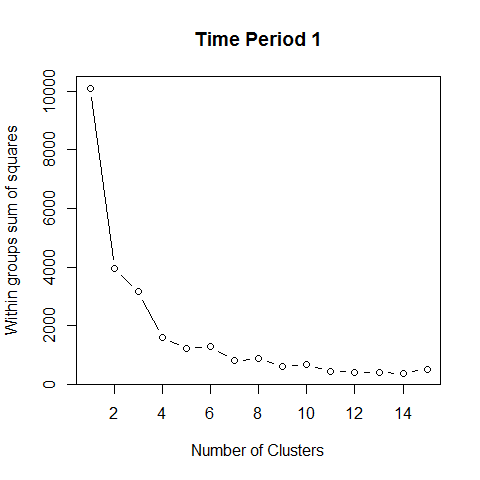
\includegraphics[width=0.32\textwidth]{images/chapter4/elbowNumberOfClusters1.png}
                 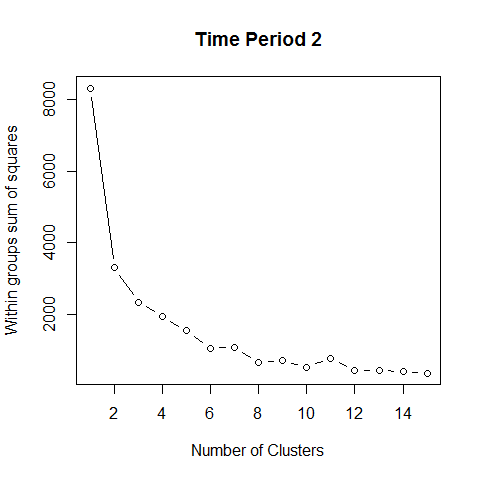
\includegraphics[width=0.32\textwidth]{images/chapter4/elbowNumberOfClusters2.png}
                 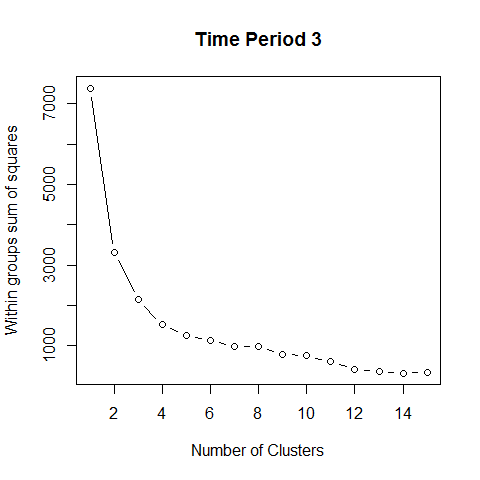
\includegraphics[width=0.32\textwidth]{images/chapter4/elbowNumberOfClusters3.png}
             }\\
             \subfigure{
                 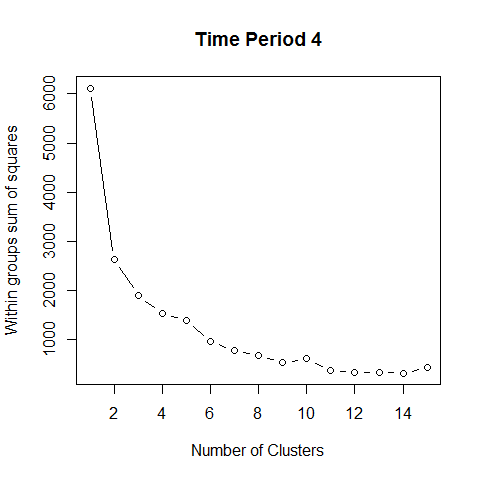
\includegraphics[width=0.32\textwidth]{images/chapter4/elbowNumberOfClusters4.png}
                 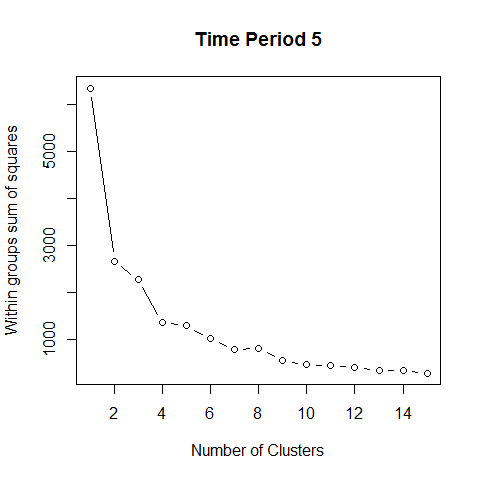
\includegraphics[width=0.32\textwidth]{images/chapter4/elbowNumberOfClusters5.png}
                 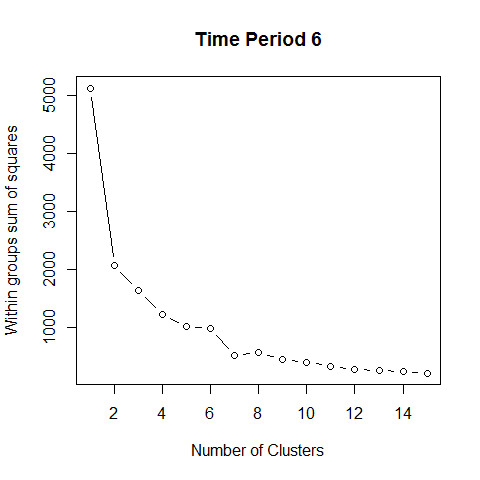
\includegraphics[width=0.32\textwidth]{images/chapter4/elbowNumberOfClusters6.png}    
             }\\
             
             \subfigure{
                 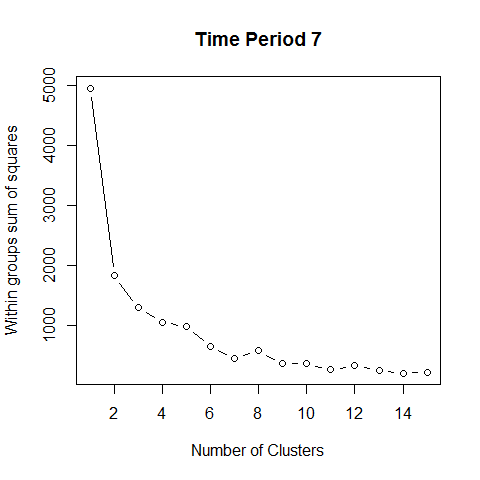
\includegraphics[width=0.32\textwidth]{images/chapter4/elbowNumberOfClusters7.png}
                 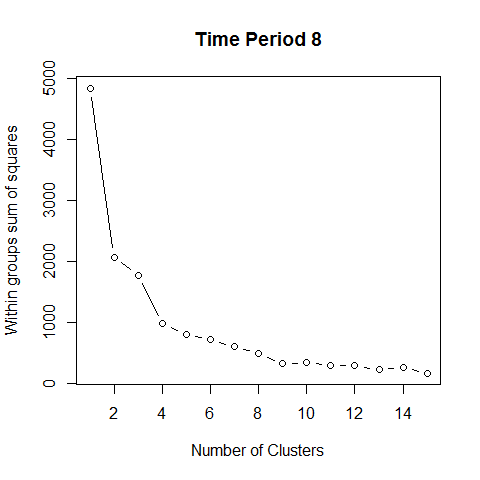
\includegraphics[width=0.32\textwidth]{images/chapter4/elbowNumberOfClusters8.png}
                 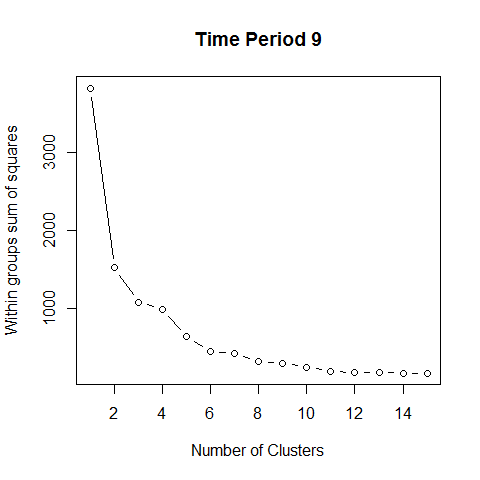
\includegraphics[width=0.32\textwidth]{images/chapter4/elbowNumberOfClusters9.png}    
             }\\
         \end{minipage}}
         \caption{Using elbow method and calculating the sum of squared errors within groups to find appropriate number of clusters for the public goods game data in each time point.}
         \label{fig:elbowNumberOfClusters}
     \end{figure}
     
     We implemented an extra test to evaluate the group memberships of players which are predicted by the clustering algorithm for cluster numbers from 2 to 15. Each of the previously clustering results was compared with economists' classifications using Rand external cluster validity. Please refer to chapter two for more information about Rand index for external cluster validity. Using the elbow method once again, the results indicate, as shown in Figure \ref{fig:elbowMemberShipAgreement}, which economists' classes are adequately represented by using four clusters. Moreover, using four clusters is also beneficial for comparison reasons with the available classification from economists.
     
     \begin{figure}[!h]
         \hfill{\begin{minipage}{\dimexpr \textwidth-2\fboxsep-2\fboxrule}% maximum allowed
                 \centering
                 \subfigure{
                     \includegraphics[width=0.32\textwidth]{images/chapter4/elbowMemberShipAgreement1.png}
                     \includegraphics[width=0.32\textwidth]{images/chapter4/elbowMemberShipAgreement2.png}
                     \includegraphics[width=0.32\textwidth]{images/chapter4/elbowMemberShipAgreement3.png}
                 }\\
                 \subfigure{
                     \includegraphics[width=0.32\textwidth]{images/chapter4/elbowMemberShipAgreement4.png}
                     \includegraphics[width=0.32\textwidth]{images/chapter4/elbowMemberShipAgreement5.png}
                     \includegraphics[width=0.32\textwidth]{images/chapter4/elbowMemberShipAgreement6.png}    
                 }\\
                 \subfigure{
                     \includegraphics[width=0.32\textwidth]{images/chapter4/elbowMemberShipAgreement7.png}
                     \includegraphics[width=0.32\textwidth]{images/chapter4/elbowMemberShipAgreement8.png}
                     \includegraphics[width=0.32\textwidth]{images/chapter4/elbowMemberShipAgreement9.png}    
                 }\\
             \end{minipage}}
             \caption{Using rand index to find the best member ship matches between clusters and classes.}
             \label{fig:elbowMemberShipAgreement}
         \end{figure}
         
 The synthetic data set is created with distinct four clusters, so its results can be comparable with the results of the public goods game data sets.
         
\subsection{Choosing External Cluster Validity Indices}
\label{sec:ChoosingExternalClusterValidityIndices}
         
As explained in the methodology section of chapter three, we propose using external cluster validity indices and area under the curve AUC to measure the changes which might occur in the behaviour of the items between multiple time points in a temporal data. Many external cluster validity indices are available \cite{Arbelaitz2012} to measure the validity of clusters produced by clustering methods compared with the natural partitions that exist. In chapter 17 of their book, Zaki et al. \cite{Zaki2014} categorised the external clustering validities into three types: matching based measures, entropy-based measures and pairwise measures. For more information on external cluster validity indices, please refer to chapter two.
         
As is the case for matching-based measures,  external cluster validity indices calculate the match of the clusters to the partitions. This means this measure is not concerned about individual element differences between clusters and partition.  This category might, therefore,  not be beneficial in calculating the changes over time.
         
The second category of external cluster validity indices, entropy-based measures, calculates the difference of entropy between clusters and ground truth partitions. This method is not concerned about individual items in the clusters and partitions. However, we used one measure of this category, Variation of Information VI, because the entropy of the clusters might be affected by the change of items within the clusters. We also used VI for comparison purposes with other indices.
         
The last category, pairwise measures, measures cluster validity by comparing the produced clusters and original labels of items' classes. As this category calculates the validity using all elements of the data set,  it may, therefore, be the most appropriate category to calculate the items' changes over time points. Three instances of pairwise measures are used in this chapter: the Jaccard Coefficient, Rand Statistic and the Fowlkes-Mallows Measure. Please refer to chapter two for more details on each of these measures.
         
Standard criteria for different external cluster validity indices must be maintained so that the final result which quantifies the amount of change in each time point reflects the actual change in the groups' items regardless of the measure used. To ensure the measures are standard, they should follow two rules (1) the scale of the measure should be between 0 and 1 (2) with 0 being the total change and 1 the perfect match between any time point and reference of behaviour. However, not all measures follow these rules. For example, in the selected measures the VI is not bound to any scale, and zero is considered as a perfect match. Thus, the results of this measure should be (1) scaled to the range of  [0-1] (2) then reversed, by subtracting the current time points' result from the maximum change which can be obtained from the data set.
         
\subsection{Using Internal Cluster Validity Indices}
         
We have considered using internal cluster Validity Indices alongside external cluster validity indices.  We tested multiple internal cluster validity indices such as Davies Bouldin index \cite{Davies1979a}, and Dunn index \cite{Dunn1973a}. However, all internal cluster validity indices are designed to measure the validity of the clusters using an \gls{ItemsAgglomeration} in the clusters and distances among clusters. This means that the Internal cluster validity indices can detect changes which are happening to the clusters in general but not the individual changes in items. We, therefore, dismissed the results produced by this method.
         
\subsection{Using Area Under the Curve}

 As explained by Fawcett \cite{Fawcett2006}, AUC calculates the area under the Receiver Operating Characteristic ROC curve and is plotted as a relationship between true positive rate and false positive rate. As this criterion uses an element-wise comparison to find the number of true positive and false positives, this measure might be useful in calculating the changes between two time points. Originally, this measure was used to demonstrate the quality of binary classification. However, a generalised method of multiple classes is presented by Hand et al. \cite{Hand2001}. Please refer to chapter two for more details on AUC.
         
AUC is designed to measure how well a classifier performs in predicting classes of elements compared with the true labels of the elements. This means, unlike pairwise external cluster validity measures, before using AUC to measure the change over time, the cluster labels of time points should be matched. There are a number of methods to match clusters \cite{Rezaei2016,Halkidi2002a}. We have used these methods:
         
\begin{itemize}
    \item Using the cluster centroids of n time point to be the suggested start centroid for the n+1 time point. However, this method only works with k--means and PAM, but it is not an option for hierarchical clustering.
    \item Using distances between centroids of the produced clusters in both time points as a reference for matching between clusters.
    \item Comparing the elements' membership in clusters between these two time points to find the matches between clusters.
\end{itemize}
         
 \subsection{Different Reference of Behaviours for Items}
 \label{sec:DifferentReferenceofBehavioursforItems}
         
This study considers three different references of behaviours.  However, in this chapter,  we will test two. They are  1) the first time point is used as a reference of behaviour for all other time points 2) The previous time point is used to be the reference of behaviour for the current time point. In the next chapter, a new classification method will be proposed to classify items in temporal data sets. This classification will be used as a reference of the items' behaviour in chapter six.
         
Each of these different references of behaviour brings different meaning and can be used in various ways. The first time point can be used as a reference of behaviour to quantify the progress of change which happens to the items in any later time points in the data set. An example of that is if we want to quantify the change of behaviour of players in PGG from the first round of the game to any round of the game.     Using the previous time point as a reference for the current time point means we aim to stepwise measure changes in items' behaviour between any time point. This can be used to measure the stability of change over time. An example of using this method is when we want to check the stability of changes that can occur in player behaviour between time points. Items' classes such as reference of behaviour can be used to quantify items' deviation from their own generalised behaviour at any time point.
         
         
         
 \section{Testing the Proposed Method}
         
We conducted this experiment to show that the proposed method can be used for measuring changes among various groups over time in temporal data. The synthetic data is created so that obvious changes of behaviour can be observed by introducing jumps for items from one group to another. The item set contains 500 items grouped into four distinct groups. The data is mutated repeatedly using jumps and jiggles 19 times to create 20 time points (the original data set is the first one). To illustrate the original and mutated data three time points are shown in Figure \ref{fig:synthesisData2}. Please refer to section \ref{CreatingaSyntheticData} in chapter three for a detailed explanation of the method of creating the data set.
         
\begin{figure}[!h]
\centering
{
    \subfigure[First time point]{
        \includegraphics[width=0.31\textwidth]{images/chapter3/synthesisDataFirst.png}\label{fig:synthesisData_first2}}
    \subfigure[Middle time point]{
        \includegraphics[width=0.30\textwidth]{images/chapter3/synthesisDataMid.png}\label{fig:synthesisData_mid2}}
    \subfigure[Last time point]{
        \includegraphics[width=0.30\textwidth]{images/chapter3/synthesisDataLast.png}\label{fig:synthesisData_last2}}}
\caption{Three time points (first, middle and last) from the 20 time points created overall. The first time point, contains 500 items and separated into four clusters, is the original data set other time points are created by mutating (jumping) items of four clusters from one cluster into another.}
\label{fig:synthesisData2}
\end{figure}
         
To test Hypothesis \ref{hypo:diffCluster}, multiple clustering methods are used in this experiment to group items in each time point of the synthetic data set. The clustering methods are chosen based on the criteria discussed in section \ref{sec:ChoosingClusteringAlgorithms}. Moreover to test Hypothesis \ref{hypo:diffCVI}, multiple external cluster validity indices and the AUC of ROC are used to measure the magnitude of changes happening to the items in the produced groups using different clustering methods. The choice of external cluster validity indices are based on the prior discussion in section \ref {sec:ChoosingExternalClusterValidityIndices}. We also tested the two types of reference of behaviour for items. To do so, all tests are run twice. The first occasion considered the first time point as the reference of behaviour and then all time points were compared with it. The second time considered previous time point as the reference of behaviour for the current time point. Please refer to section \ref{sec:DifferentReferenceofBehavioursforItems} for more details.

Using this method, both clustering techniques, external cluster validity indices, and reference of behaviour, produce a result of an array of values which quantify the difference between each time point and the reference of behaviour. These values can be reported as a list of values, or a table. However, to obtain an idea of the degree of change of items of groups through time points, an x,y chart can be used with time points as x-axes and the magnitude of change values scaling from 0 to 1 as y-axes. Figure \ref{fig:test_ChangeMeasuers_Firs} shows results of k--means, PAM, c--means and hierarchical clustering methods using the first time point as the reference of behaviour to calculate the magnitude of changes which happen to the groups of items in consequent time points in the test data set. The amount of change is measured by using different external cluster validity indices and AUC of ROC. Moreover, Figure \ref{fig:test_ChangeMeasuers_Cons} shows results for the proposed method using the same clustering techniques and external cluster validity indices although it uses the previous time point as the reference of behaviour for the current one.

Figure \ref{fig:test_ChangeMeasuers_Firs} shows a gradual shift from the first time point as each new time point introduces further mutations for the data set and, hence, further drifting from the original location of the items. While all measures confirm the gradual change of progressing time points, however, not all of them react in the same way. The major noticeable difference is that FM and Jaccard are overreacting to the changes and show high sensitivity to it. As the VI values are scaled and flipped, they correspond to fit the rules laid out in section  \ref{sec:ChoosingExternalClusterValidityIndices}. Results are, therefore, shown in a very saturated scale as the lowest point become zero due to the scaling and flipping. However, the actual changes are a small percentage of the overall items suggesting that these scales of change by the two measures could be due to the original design of these two measures to show the difference between clusterings and real classes. Moreover, all results of the hierarchical clustering show a slightly different change pattern than other clustering methods. Another noticeable result is that k means clustering shows an increased sensitivity to the changes between 14 and 15 time points. The same sensitivity is not depicted by other clustering algorithms.
         
\begin{figure}[!h]
\hfill{\begin{minipage}{\dimexpr \textwidth-2\fboxsep-2\fboxrule}% maximum allowed
        \centering
        \subfigure[K--means Clustering]{
            \includegraphics[width=0.45\textwidth]{images/chapter4/test_kmeansClusters_Firs.png}
        }
        \subfigure[PAM Clustering]{
            \includegraphics[width=0.45\textwidth]{images/chapter4/test_PAMClusters_Firs.png}
        }\\
        
        \centering
        \subfigure[C--means Clustering]{
            \includegraphics[width=0.45\textwidth]{images/chapter4/test_cmeansClusters_Firs.png}
        }
        \subfigure[Hierarchical Clustering]{
            \includegraphics[width=0.45\textwidth]{images/chapter4/test_hierClusters_Firs.png}
        }\\
        
    \end{minipage}}
    \caption{Results of various clustering methods using the first time point as a reference of behaviour to calculate the magnitude of changes which happen to the groups of items in consequent time points in the test data set. The amount of change  is measured by using different external cluster validity indices and AUC of ROC.}
    \label{fig:test_ChangeMeasuers_Firs}
\end{figure}
             
             
Figure \ref{fig:test_ChangeMeasuers_Cons} shows the difference between any two consequent time points. PAM and c--means clustering methods created visually similar results while k--means and hierarchical clustering produced very different results. While all clustering methods are producing a greater change between time points 13-15,  k--means, however,  shows an extreme change in the same time periods. In these results, VI shows exaggerated differences between time points. However, FM and Jaccard results display the difference between time points more than AUC and Rand. AUC and Rand results might reflect the reality of the changes, but the changes become unnoticeable due to the small scaling.
             
\begin{figure}[!h]
\hfill{\begin{minipage}{\dimexpr \textwidth-2\fboxsep-2\fboxrule}% maximum allowed
        \centering
        \subfigure[K--means Clustering]{
            \includegraphics[width=0.45\textwidth]{images/chapter4/test_kmeansClusters_Cons.png}
        }
        \subfigure[PAM Clustering]{
            \includegraphics[width=0.45\textwidth]{images/chapter4/test_pamClusters_Cons.png}
        }\\
        
        \centering
        \subfigure[C--means Clustering]{
            \includegraphics[width=0.45\textwidth]{images/chapter4/test_cmeansClusters_Cons.png}
        }
        \subfigure[Hierarchical Clustering]{
            \includegraphics[width=0.45\textwidth]{images/chapter4/test_hierClusters_Cons.png}
        }\\
        
    \end{minipage}}
    \caption{Results of various clustering methods using the previous time point as reference of behaviour to calculate the magnitude of changes which happen to the groups of items in consequent time points in the test data set.}
    \label{fig:test_ChangeMeasuers_Cons}
\end{figure}
                 
                 
                 
The Friedman test is used to validate Hypothesis \ref{hypo:diffCluster} on the proposed method for measuring changes over time using acquired results from the synthetic data set. The p.value of the four samples for measuring changes of time points against the original data set is 4.947325e-14 and p.value for measuring changes of current time points against the previous time point is 1.895672e-14. This means, in both cases, we can not reject the null hypothesis, and hence, the samples are different. However, a closer look at the results by comparing every two samples of different clustering methods using Wilcoxon tests reveals (see Table \ref{tab:Cluster_Pvalue_Test}) that all p.values are higher than 0.05 for the samples used the first time point as the reference of behaviour. For those samples which using previous time point as the reference of behaviour, only hierarchical clustering produced p.values less than 0.05 when compared with other samples. This means all three clustering methods are producing the same results for measuring changes over time. Given that, we can consider Hypothesis \ref{hypo:diffCluster}  to hold true especially given all clustering methods are confirming that the items inside the groups are changing gradually over time. The difference is only in the sensitivity to the change, an aspect of the clustering method.

\begin{table}[!h]
    \ra{1.3}
    \small
    \centering
    \caption{ P-values of Wilcoxon-test for each pair of clusters.}
    \label{tab:Cluster_Pvalue_Test}
    \begin{tabular}{llll}
        \toprule
        \textbf{Clustering1} & \textbf{Clustering2}  & \textbf{p-Value First} & \textbf{p-Value Consequent} \\ \midrule
        k--means      & c--means       & 0.9778971     & 0.6262925          \\ 
        k--means      & PAM          & 0.7868127     & 0.8050843          \\ 
        k--means      & hierarchical & 0.5369699     & 0.000704285        \\ 
        c--means      & PAM          & 0.7555338     & 0.7776328          \\ 
        c--means      & hierarchical & 0.4877342     & 3.17E-05           \\ 
        PAM         & hierarchical & 0.6903287     & 4.68E-05           \\ 
        \bottomrule
    \end{tabular}
\end{table}


To validate Hypothesis \ref{hypo:diffCVI}, the similarity of result samples produced by different external cluster validity indices have to be measured. We used the Friedman test to check if all the results are similar to the null hypothesis that assumes similarity for the produced results in measuring the amount of change for all time points using different external cluster validity indices or AUC. Two p-values are produced. The first p-value = 5.232651e-44 for the samples which are produced by measuring the behaviour of each time point compared to the first time point. The second p-value = 1.416841e-53 for the results which are produced by comparing each time point with its successor.  In both cases, p-values are smaller than 0.05.  The null hypotheses should, therefore, be rejected as the samples are different.  Moreover, we conducted a Wilcoxon test on the samples to take a closer look at the results of every pair of two samples produced with different measures. As shown in Table  \ref{tab:ECVI_Failed_Pvalue_Test}, the p-values (except for the AUC and Rand pair) are smaller than 0.05 which indicates that these pairs are different from each other. This means that different measures are producing significantly different results. Hence, Hypothesis \ref{hypo:diffCVI} can not be true. So, further examination of the results is required to check whether the proposed method can be used to measure changes over time or not.

However, despite the measures producing different results, as proved by using different statistical tests, we can see from figures \ref{fig:test_ChangeMeasuers_Firs} and \ref{fig:test_ChangeMeasuers_Cons} that all measures indicate the gradual change in the data with different sensitivities to the amount of change. As the data is synthesised and new time points are created by mutating the current time point, we can, thus, confirm that the results reflect the gradual change which already exists in the data. Therefore, the difference between samples might be a direct result of the different sensitivities which each measure is created for, and included in its method of calculating differences in group similarities between predicted results and true labels of the items.

Measures with different sensitivities proved to be a positive aspect of the proposed method for measuring changes over time in various situations as it enables us to control the amount of sensitivity needed for a specific situation or application. For example in Figure \ref{fig:test_ChangeMeasuers_Firs}, Rand and AUC measures reflect the amount of change well, while in Figure \ref{fig:test_ChangeMeasuers_Cons} Jaccard and FM can highlight changes which can not be detected by the previous two measures.



\begin{table}[!h]
    \ra{1.3}
    \small
    \centering
    \caption{P-values of Wilcoxon-test for each pair of external cluster validity indices and AUC.}
    \label{tab:ECVI_Failed_Pvalue_Test}
    \begin{tabular}{llll}
        \toprule
        \textbf{Clustering1} & \textbf{Clustering2}  & \textbf{p-Value First} & \textbf{p-Value Consequent} \\ \midrule
        Rand      & Jaccard  & 1.947533e-17     & 2.182083e-13          \\ 
        Rand      & FM       & 1.857682e-11     & 4.051658e-07          \\ 
        Rand      & VI       & 4.131331e-13     & 9.372113e-24          \\ 
        Rand      & AUC      & 0.9251302        & 0.5177034             \\ 
        
        Jaccard   & FM       & 3.865308e-08     & 3.565382e-06          \\ 
        Jaccard   & VI       & 1.977779e-18     & 1.242547e-22          \\ 
        Jaccard   & AUC      & 1.103106e-17     & 2.012194e-13          \\ 
        
        FM        & VI       & 1.956715e-15     & 3.196178e-23          \\ 
        FM        & AUC      & 2.114171e-11     & 1.110287e-06          \\ 
        
        VI        & AUC      & 3.718286e-13     & 1.051501e-23          \\     
        \bottomrule
    \end{tabular}
\end{table}

To be able to use the proposed method for measuring changes over time in temporal data, it should, at least, be proven that each measure independently from other measures can produce consistent results for different clustering methods. Another test is conducted to check if a measure can produce consistent results across multiple clustering methods. The results for each measure produced by different clustering algorithms are compared, and the p-value for the Wilcoxon test is produced as shown in Table \ref{tab:ECVI_Pvalue_Test}. P-values of each pair of the produced samples are higher than 0.05 except for hierarchical clustering when using previous time point as a reference of behaviour (consequent test). This means we can not reject the null hypothesis because the results of measures are consistent across multiple clustering methods. That the p-value is not smaller than 0.05 in hierarchical clustering might be because hierarchical clustering itself produces different groups than other clustering methods as has been previously proven in this section.


\begin{table}[!h]
    \ra{1.3}
    \small
    \centering
    \caption{P-values of Wilcoxon-test for each pair of external cluster validity indices or AUC.}
    \label{tab:ECVI_Pvalue_Test}
    \begin{tabular}{rllllll} \toprule
        Cluster1  & Cluster2   & Rand        & Jaccard     & FM          & VI          & AUC        \\ \midrule
        \multicolumn{1}{l}{\textbf{First}}       \\        
        k--means       & c--means        & 0.930085   & 0.930085   & 0.930085   & 1           & 0.941807  \\
        k--means       & PAM           & 0.883816   & 0.906934   & 0.906934   & 0.906934    & 0.165448  \\
        k--means       & hierar           & 0.704262   & 0.704262   & 0.682708   & 0.704262    & 0.085021  \\
        c--means       & PAM           & 0.965026   & 0.988339   & 0.988339   & 0.91851     & 0.188877  \\
        c--means       & hierar           & 0.579058   & 0.579058   & 0.579058   & 0.682708    & 0.08502   \\
        PAM          & hierar           & 0.579058   & 0.579058   & 0.579058   & 0.682708    & 0.539772  \\
        \multicolumn{1}{l}{\textbf{Consequent}}\\        
        k--means       & c--means        & 0.558817   & 0.558817   & 0.558817   & 0.619407    & 0.609161  \\
        k--means       & PAM           & 0.529826   & 0.539462   & 0.539462   & 0.640234    & 0.578892  \\
        k--means       & hierar           & 0.00319    & 0.003505   & 0.003504   & 0.018246    & 9.14E-05  \\
        c--means       & PAM           & 0.976681   & 0.98834    & 0.98834    & 0.98834     & 0.214412  \\
        c--means       & hierar          & 6.34E-05   & 6.34E-05   & 6.34E-05   & 0.000787    & 8.05E-07  \\
        PAM          & hierar          & 4.94E-05   & 4.94E-05   & 4.94E-05   & 0.001192    & 6.92E-06  \\
        
        \bottomrule
    \end{tabular}
\end{table}

In this section, we demonstrated and proved that using different clustering techniques will produce similar results for measuring changes over time. We also proved that using the same measure (that is external cluster validity indices or AUC of ROC) produces consistent results across all clustering methods. This is an indication that the proposed method can be used to measure changes over time and produce a single value which indicates the amount of change that happens to items' membership in the available groups at different time points.


\section{Measuring Players' Strategy Change over Time}
The main objective of this experiment is to quantify how players' change in strategy in the public goods game can contribute to the understanding of the players' behaviour and present a tool for economists to measure the amount of change for different set-ups of their experiment. Another objective of this experiment is to demonstrate the ability of the proposed method to produce quantifiable measures for changes in items. In the temporal data and provide interpretable results. We compare the results and findings of our method with the MONIC method which is originally used to measure cluster changes in a data stream  \cite{Spiliopoulou2006}.

In section \ref{PublicGoodsGamesData} of chapter three, two data sets of PGG are introduced. For this experiment,  both data sets are used to measure players behaviour and strategy change during the consequent rounds of the game. The attribute of players own contribution and their expectation of other players' contribution at each time point are used by this method to find the magnitude of the change. These two data sets have different groups of players and different lengths as the first data set is 10 rounds length and the second is 27. Therefore, these two data sets are used separately and treated as different data sets in this experiment. Based on the previous discussion in section \ref{sec:Choosing-Number-of-Clusters}, we used four clusters to cluster players in each time point using k--means, PAM, c--means and hierarchical clustering methods.These methods were selected based on our discussion in section \ref{sec:ChoosingClusteringAlgorithms}.

As both data sets of PGG share the same experiment settings and setup, it can be hypothesised that the results of the behaviour change should be consistent with regards to the length of the experiment which, in turn,  might affect the behaviour of players \cite{Figuieres2010}. While we use all previously selected external cluster validity indices as in section \ref{sec:ChoosingExternalClusterValidityIndices} and AUC of ROC. We will, however, depend on AUC and Rand results to compare the behaviour of players in these two different data sets as we demonstrated that these two measures produce more consistent results than the rest of the measures.


\subsection{Using Proposed Method}

Prior to the analysis of the players' behaviour, we checked both Hypothesis \ref{hypo:diffCluster} and \ref{hypo:diffCVI} using real data sets. Using p-value, as described in the previous section, similarities between results of different clustering and external cluster validity indices are tested. P-value results are shown in Appendix \ref{App:P-Values-for-Public-Goods-Game}. While slightly different results are produced especially for 27 period data set, the results are consistent with the results of synthetic data. This can be considered as additional evidence that the presented method for measuring changes over time can be used with real data sets.

Different types of reference point reveal different aspects of players' strategy change. By using the first time point as the reference of behaviour, we can detect drift of players' behaviour from the initial expectation and contribution. As shown in Figure \ref{fig:game10_ChangeMeasuers_Firs} for 10 rounds data set and Figure \ref{fig:game27_ChangeMeasuers_Firs} for 27 rounds, players in both data sets are gradually drifting away from their initial game plan and expectation. This trend can be seen with all four clustering methods with the different measurement methods of external cluster validity indices and AUC. Because the results of AUC and Rand are consistent across all clustering methods, we used AUC to calculate the linear regression of the results. The negative results of linear regression is an indication that players increase their behaviour of drifting away from their original gameplay.

By using the previous time point as the reference of behaviour, we can measure the amount of change between any two consecutive time points. This allows detection of players' behaviour transition from one time point to another. Figure \ref{fig:game10_ChangeMeasuers_Cons} of the 10 rounds data set shows that players strategy change from one time point to another is constant. This is indicated by the linear regression of AUC and Rand measures. In contrast Figure \ref{fig:game27_ChangeMeasuers_Cons} of 27 rounds shows that the change between time points is decreasing throughout the progress of the game. 

At first glance, the results of 10 and 27 rounds data sets are not consistent. However, after taking a closer look at the results, we can detect that the players' behaviour change in 27 rounds data set is stable without any decrease until round 10 of the game. As shown in Figure \ref{fig:contributionRound27} this decrease might be due to the fact that most of the players dropped their contribution to zero when they reached round 10. This means there is no room for further change left in the game except some players randomly start to increase their contribution again but the rise is not constant, so after round 10 we detect less change than expected.

\begin{figure}[!h]
\hfill{\begin{minipage}{\dimexpr \textwidth-2\fboxsep-2\fboxrule}% maximum allowed
    \centering
    \subfigure[K--means Clustering]{
        \includegraphics[width=0.45\textwidth]{images/chapter4/game10_kmeansClusters_Firs.png}
    }
    \subfigure[PAM Clustering]{
        \includegraphics[width=0.45\textwidth]{images/chapter4/game10_pamClusters_Firs.png}
    }\\
    
    \centering
    \subfigure[C--means Clustering]{
        \includegraphics[width=0.45\textwidth]{images/chapter4/game10_cmeansClusters_Firs.png}
    }
    \subfigure[Hirarchical Clustering]{
        \includegraphics[width=0.45\textwidth]{images/chapter4/game10_hierClusters_Firs.png}
    }\\
    
\end{minipage}}
\caption{Results of various clustering methods using the first time point as reference of behaviour to calculate the magnitude of changes which happen to the groups of items in consequent time points in the 10 rounds PGG data set.}
\label{fig:game10_ChangeMeasuers_Firs}
\end{figure}
    
    
    
\begin{figure}[!h]
\hfill{\begin{minipage}{\dimexpr \textwidth-2\fboxsep-2\fboxrule}% maximum allowed
        \centering
        \subfigure[K--means Clustering]{
            \includegraphics[width=0.45\textwidth]{images/chapter4/game10_kmeansClusters_Cons.png}
        }
        \subfigure[PAM Clustering]{
            \includegraphics[width=0.45\textwidth]{images/chapter4/game10_pamClusters_Cons.png}
        }\\
        
        \centering
        \subfigure[C--means Clustering]{
            \includegraphics[width=0.45\textwidth]{images/chapter4/game10_cmeansClusters_Cons.png}
        }
        \subfigure[Hirarchical Clustering]{
            \includegraphics[width=0.45\textwidth]{images/chapter4/game10_hierClusters_Cons.png}
        }\\
        
    \end{minipage}}
    \caption{Results of various clustering methods using the previous time point as reference of behaviour to calculate the magnitude of changes which happen to the groups of items in consequent time points in the 10 rounds PGG data set.}
    \label{fig:game10_ChangeMeasuers_Cons}
\end{figure}
        
        
As we hypothesised in the previous section, player behaviour has to be consistent in both data sets. The results for measuring changes using the first time point as the reference of behaviour are compatible as players' contribution drops gradually in both cases. The results of using the previous time point as the reference of behaviour show that players strategy change is constant until round 10. In 27 rounds data set, most players' contribution after round 10 dropped to zero meaning there is no room for further change in their strategy. Hence, the amount of change in their strategy decreases and their game pattern starts to become similar between any two consequent time points. These results show that the proposed hypothesis holds true. This is yet another indication that the proposed method produces consistent results for similar situations.


\begin{figure}[!h]
\hfill{\begin{minipage}{\dimexpr \textwidth-2\fboxsep-2\fboxrule}% maximum allowed
        \centering
        \subfigure[K--means Clustering]{
            \includegraphics[width=0.45\textwidth]{images/chapter4/game27_kmeansClusters_Firs.png}
        }
        \subfigure[PAM Clustering]{
            \includegraphics[width=0.45\textwidth]{images/chapter4/game27_pamClusters_Firs.png}
        }\\
        
        \centering
        \subfigure[C--means Clustering]{
            \includegraphics[width=0.45\textwidth]{images/chapter4/game27_cmeansClusters_Firs.png}
        }
        \subfigure[Hirarchical Clustering]{
            \includegraphics[width=0.45\textwidth]{images/chapter4/game27_hierClusters_Firs.png}
        }\\
        
    \end{minipage}}
    \caption{Results of various clustering methods using the first time point as reference of behaviour to calculate the magnitude of changes which happen to the groups of items in consequent time points in the 27 rounds PGG data set.}
    \label{fig:game27_ChangeMeasuers_Firs}
\end{figure}
            
            
The results of the proposed method for both data sets are compatible with the findings of economists \cite{Fischbacher2010,Hoice2008,Chaudhuri2006}. However, this method provides a tool which enables them to quantify changes in players behaviour. Quantifying behaviour change is important so they can measure the nuanced differences between various gameplay setups like the length of the rounds, the percentage of the rewards from the public project, and knowing the identity of other players.




\begin{figure}[!h]
\hfill{\begin{minipage}{\dimexpr \textwidth-2\fboxsep-2\fboxrule}% maximum allowed
        \centering
        \subfigure[K--means Clustering]{
            \includegraphics[width=0.45\textwidth]{images/chapter4/game27_kmeansClusters_Cons.png}
        }
        \subfigure[PAM Clustering]{
            \includegraphics[width=0.45\textwidth]{images/chapter4/game27_pamClusters_Cons.png}
        }\\
        
        \centering
        \subfigure[C--means Clustering]{
            \includegraphics[width=0.45\textwidth]{images/chapter4/game27_cmeansClusters_Cons.png}
        }
        \subfigure[Hirarchical Clustering]{
            \includegraphics[width=0.45\textwidth]{images/chapter4/game27_hierClusters_Cons.png}
        }\\
        
    \end{minipage}}
    \caption{Results of various clustering methods using the previous time point as reference of behaviour to calculate the magnitude of changes which happen to the groups of items in consequent time points in the 27 rounds PGG data set.}
    \label{fig:game27_ChangeMeasuers_Cons}
\end{figure}
    
\subsection{Using MONIC}
    
We used MONIC\footnote{Available at http://infolab.cs.unipi.gr/people/ntoutsi/monic.html} to gain more insight into the public goods games data and to compare our results with the existing methods of measuring cluster changes in different time points. The data for each time period were clustered separately using k--means with four clusters. The clustering was carried out on the main temporal attributes of the data, namely belief and contribution. Then the data and cluster labels of items in each consequent pair of time points were fed to the MONIC algorithm to calculate changes to clusters from one time point to another. The method calculated the number of survived, appeared and disappeared clusters, as shown in figures \ref{fig:monic10} and \ref{fig:monic27}, for the ten rounds of the game.
    
    
In the 10 rounds data set, the number of survived clusters reduced from four clusters between the first and second time points until it reached zero, while new clusters appeared in the middle of the fifth and sixth game rounds. Then the number rose again until the end of the game. This might be due to the fact that players are changing their strategies and exploring new options until they ultimately settle on a certain strategic pattern. This change is consistent with our findings, as the measures slightly increase between the fifth and seventh time points, which might be an indication of players changing their strategy back to their original one. As Keser and Winden \cite{Keser2000} suggest, this change might be due to the players responding to the average contribution of other players in the previous round.
    
\begin{figure}[!h]
    \centering
    \includegraphics[width=0.75\textwidth]{images/chapter4/monic10.png}
    \caption{Number of survival, appearance and disappearance of clusters between every tow consequent time points for ten rounds public goods game as measured by MONIC.}
    \label{fig:monic10}
\end{figure}

The results for the 27 rounds data set is not straightforward as the numbers of cluster survivals, appearances and disappearances change more frequently. However, the cyclic pattern of increasing and decreasing number of survived clusters might be an effect of changing players' strategies or due to the underlying algorithm, as it provides an ageing factor to the items.

\begin{figure*}[th]
    \centering
    \includegraphics[width=1.0\textwidth]{images/chapter4/monic27.png}
    \caption{Number of survival, appearance and disappearance of clusters between every tow consequent time points for 27 rounds public goods game as  measured by MONIC.}
    \label{fig:monic27}
\end{figure*}

As the MONIC algorithm was originally introduced to detect cluster changes in data streams, it uses an ageing factor which reduces the effect of older items in the cluster and removes items older than two time points \cite{Spiliopoulou2006}. This ageing factor is essential for the algorithm to keep up-to-date with the flowing data stream and provide the right results for the current status of the clusters. However, this might not be useful for public goods games data, as there is a fixed number of players. This might result in the removal of players who stay in the same cluster for long time points. The effect of the ageing might not be obvious in the 10 rounds game due to the limited number of time points, but it might still undermine players' strategies.
                                 
While the proposed method assumes a fixed number of clusters to calculate the change in items membership, the MONIC algorithm is an effective method for gaining insights into the available clusters and their stability by measuring the number of survived clusters between two time points. However, it does not measure a number of items drifting from one cluster into another, which can be detected by the proposed method, as it introduces a specific ratio between each consequent time point, indicating the amount of change was happening to the items in the clusters by calculating their membership change among clusters.
                                 
MONIC can be compared with the proposed method especially the case of previous time point as a reference of behaviour as both of these methods compare the current clusters with the previous time point. The regression result for the average of cluster moves (appear, disappear and survive) is near to zero, which is compatible with the proposed method results using the previous time point as a reference of behaviour except for 27 rounds clustered by PAM and hierarchical clustering. By comparing results from the proposed method and MONIC, we can conclude that the players slightly and gradually change their cluster membership. However, the magnitude of change is stable from one time point to another. The proposed method provides an exact number for the change while the MONIC presents overall clusters movement and change.
                                 
\section{Summary}

The primary purpose of this chapter is to answer two of the main questions of the study. The first question is: Can we use the proposed method in chapter three to measure changes over time? The second question is: Do players of PGG behave as predicted by economists? As presented in chapter three, the proposed method consists of two main steps. The first step is to cluster items at each time point,  and the second step is to measure changes happening in the clusters of each time point using a reference of behaviour. Many types of reference of behaviour for items in the data set can exist; in this chapter, we tested two, namely the first time point and previous time point.

To answer the first question we checked the validity of hypothesis  \ref{hypo:diffCluster} and \ref{hypo:diffCVI}. Laid out in the first chapter, they are:
\begin{itemize}
    \item To prove that the above proposition is valid the results of different external clustering indices and AUC should be consistent.
    \item Using different clustering algorithms will not produce a significant difference in the final result of quantifying the changes over time as long as same clustering algorithm is used at both time points.
\end{itemize}
These two hypotheses examine the main aspects of the proposed method for measuring items' changes over time in temporal data. If these two hold true, then they can be presented as evidence which proves that the proposed method is working adequately and consistently.


To check the validity of these two hypotheses, we used the synthetic data which was introduced in chapter three. Prior to the experiment of testing the proposed method, the rationale for selecting certain clustering methods and external cluster validity indices is presented. It is crucial to make sure that the appropriate range of clustering methods are used so that items at each time point are clustered appropriately. We chose clustering methods which mainly separate items according to their distance from each other; the clusterings used are k--means, c--means, PAM and hierarchical clustering for this purpose. For external cluster validity indices,  we have mainly used the matching based methods of Jaccard Coefficient, Rand Statistic and Fowlkes-Mallows Measure. We have also used the Variation of Information VI method, which is an example of a statistical-based model, and AUC of ROC with players to measure the efficiency of classification.

Tests of the synthetic data using the proposed method with suggested clustering and external cluster validity indices multiple sample sets of results are produced. By using p-value for Wilcoxon-test, we demonstrated that each pair of results is similar to each other except for some hierarchical clustering cases. This similarity proves that the results of proposed method are consistent regardless of the clustering method used. This, therefore, verifies the validity of hypothesis  \ref{hypo:diffCluster}. While the similarity between different external cluster validity indices did not hold true, each external cluster validity indices result, however, proved to be similar across different clustering algorithms meaning the results of the external cluster validity indices are consistent but with different sensitivities to the change of items. After conducting these tests, it can be concluded that the proposed method can be successfully used to measure and quantify changes of items in temporal data.

To answer the second question, we used the proposed method on both PGG data sets introduced in chapter three. The same choice of clustering methods and external cluster validity indices are used in the process of quantifying players' strategy change. Four clusters are used of players in each time point because economists have categorised players into four groups in their studies. The four-cluster model was a viable choice as we tested the data using the Elbow method to determine the number of clusters in the data sets. The results showed that the players' strategy change when approaching the end of the game. However, the change itself between any two time point is constant on average. This result corresponds with economists' conclusions.


To gain another perspective on the players' strategy change, we used the MONIC method which was created to detect cluster change in data streams. The results showed that the clusters periodically appear and disappear through data points in the temporal data of PGG. This is an indication that the players' strategy changes as new clusters are emerging and others vanishing. Moreover, the unstable number of survived clusters is an indication that the players are not changing their strategy homogeneously and their reaction varies from each other. While the MONIC method provides a new perspective on the data set, however, it is not possible to directly compare it with the results of our proposed method because they consider different aspects of the data. The proposed method quantifies the amount of individual items exchange between clusters while MONIC shows the changes which are happening to the clusters in general.

In this chapter, we made a comparison between two different references of behaviour for items in temporal data, namely the first time point and the previous time point of the temporal data set. However, another reference of rehavior is proposed in chapter three which is the  general behaviour across all time points. This type of reference of rehavior is possible if the class of each item is known in the temporal data. In chapter five, we propose a new algorithm to classify items in a temporal data by optimising rules for classes provided by experts or human agents. In chapter six, we will use the produced classes of items as the reference of rehavior to measure changes in items.



\chapter{Optimizing Temporal Rule-Based Classification}
\label{Chap:Optimizing}

\section{Introduction}

This chapter answers the question posed in chapter one regarding the players' classification in the Public Goods Game data sets. The aim is to compare the Optimizing Temporal Rule-Based Classification proposed in chapter three section  \ref{sec:Temporal-Rule-Based-Classification} against the available classification method which is used by economists \cite{Fischbacher2001}. This comparison is formed into a Hypothesis \ref{hypo:proposedClassification} in chapter one. If this hypothesis holds true, this means our proposed method is performing better than the available classification method.

After classifying players with the proposed method, we use their new classes to answer two more questions about players behaviour. The first question concerns consistency of players strategy in various length of the game. To answer this question, we will check the validity of Hypothesis \ref{hypo:lengthOftheGame} as it states that the length of the game does not affect player strategy. The second question concerns using the overall general behaviour as Reference of Behaviour as our Hypothesis \ref{hypo:overallBehavoiur} in chapter one states that using overall behaviour as a reference of behaviour is more stable than the other two methods; the first time point and the previous time point. If this hypothesis holds true, so measuring changes over time can be performed reliably regardless of the underlying clustering and external cluster validity indices.

 

Hypothesis \ref{hypo:proposedClassification} indicates that using flexible rules by experts and then later optimising and specifying these rules will generate classes which are more representative of player's behaviour during the game. While this hypothesis is specific about the domain of the data set namely a public goods game, the proposed classification method can, however, be used on data sets with similar properties.  For example, stock market price data, students' performance over the years and effects of drugs on patients. In chapter six, we will classify stock market data using the proposed classification method.

The proposed classification method has two main steps. The first step uses specific definitions from field experts for classes which exist for items. These definitions are based on aggregated attributes of the temporal data. The second step is the optimisation process. In this step, the best possible classifier for the items will be selected. The best classifier is a classifier which can produce the most compacted classes of items (players) at each time point in the temporal data. The compactness of the classes is calculated by using a cost function which is based on the overall dispersal of items in each class. Classes' dispersal can be measured by using internal cluster validity indices like the Dunn Index, distance measures like Euclidean distance or statistical measures such as standard deviation.

In this chapter, we use brute force to find the best classifier. Brute force is simple and can solve classification in a relatively reasonable time for the available public goods game data sets. However, it can not perform optimally with a larger amount of data. Therefore, in the next chapter, we will replace the brute force with a heuristic method, namely differential evolutionary algorithm DEA, to optimise rules of the classifier.


\section{Background}
Most rule-based classifications use the  'if..else..' form to classify underlying data, which is conducive for easier comprehension  \cite{Negnevitsky2002}. The rules can be learned through examples or provided by an expert \cite{Wang1992}. As explained below, many different data mining and analysis methods use rule-based systems for classification. 

Rule-based classifications are used in fuzzy systems. For example Cordon et al. \cite{Cordon1999} proposed a new Fussy Reasoning Method (FRM) with better optimisation for the system, whereby the rules do not lose their comprehensibility. Ishibuchi \cite{Ishibuchi1999} compared two kinds of voting schemes for fuzzy rule-based classification.

Experts use common sense and vague terms to solve problems and classify situations/items, while an expert system that tries to simulate human experts uses logic to conclude decisions instead of hard programmed solutions \cite{Negnevitsky2002}. A number of expert systems that rely on rule-based logic have been introduced \cite{Styvaktakis2002}.

Many other methods have been introduced that use rule-based systems for classification, like \cite{Giacometti2008}, which proposed a generic classifier construction algorithm (ICCA). \cite{Qin2009} proposed an algorithm for a rule-based classifier that can extract rules from uncertain data, and used probability estimation for rule learning, inspired by the use of probabilities to construct decision trees.

To classify players in the public goods data sets, economists use players' contribution tables \cite{Fischbacher2001}. In this table, players state their intent for contribution in response to the rounded average contribution of other co-players. Thus, this table consists of players intended contribution conditioned by the contribution of other players ranging from 0 to 20. According to the players' response, economists classify them into four classes which are conditional co-operator, free riders, triangle contributors and others.

However, classifying players according to the contribution table which has been completed by the players prior to the game rounds might not represent players' actual behaviour during the game. This table ignores players' real contribution in the game rounds, which might change during games due to the change in their strategy as a result of their experience from previous game rounds.

There are many well known temporal classification methods which use either dynamic time warping \textbf{DTW} \cite{Berndt1994} or Euclidean distance to classify time series data sets. Examples of temporal classifiers such as Douzal-Chouakria et al. \cite{Douzal-Chouakria2012} used decision trees, Vincent S. Tseng et al. used Naive Bayes sequence classifier \cite{Tseng2009} and Ranganatha Sitaram et al. used  Support Vector Machine \textbf{SVM} as a temporal classifier with different kernels \cite{Sitaram2007}. However, all these methods require training set samples which are necessary to build their classifier instead of following experts definition to classify items in the temporal data. 

The available data sets for public goods games do not contain labels for players that reflect their behaviour during the game because experts use contribution tables to classify players. However, these tables are not directly related to their behaviour. Using a static contribution table is easier for economists to classify players as they can follow players answers manually or using simple methods. This simplified method can not be done with the temporal data even though it better reflects player behaviour. In chapter two, multiple examples are presented for methods of extracting rule-based classifiers using genetic  \cite{McAulay1994}, evolutionary algorithms \cite{Orriols-Puig2009} and SVM \cite{Nunez2006}. However, these methods require training data sets to build the classifier. 
 

\section{Approach}

The proposed classification method consists of two main steps; rule generation and rule optimisation, as shown in figure  \ref{fig:classificationProcess}. The optimised rules can be reconstructed as a decision tree.  As explained in chapter two, decision trees and rule-based classifiers can interchangeably represent each other. However, rule-based representation is preferable to humans as they are more intuitive and they might also be more efficient than their counterparts of decision trees.

In the subsections below we will detail the process of the rule generation and the methods of determining the number of classes and limits of each class. Then, we discuss the optimisation process and the parameters which are to be optimised as well as methods for measuring the optimum classifier such as using internal cluster validity indices and Euclidean distance among items. Finally, we will lay out a comparison method between the results of the proposed classification method and available classification for players of the public goods game.

\begin{figure}[!h]
    \centering
    \includegraphics[width=0.9\textwidth]{images/chapter5/classificationProcess.png}
    \caption{An illustration of the proposed classification algorithm and its relation with temporal data and their aggregates.}
    \label{fig:classificationProcess}
\end{figure}


\subsection{Choosing Initial Limits for Classes}
\label{sec:Choosing_Initial_Limits_for_Classes}
For a selected number of classes, every class has a limit in each of the aggregated (non-temporal) attributes which are used in the classification rules. A limit is start and end values of a class of a certain attribute or dimension, and these can be represented by [min, max] pairs. As we mentioned in chapter three section \ref{sec:Generating-Initial-Rules}, classification rules are formulated in a nested if-else fashion to evaluate items' class as well as classes of priorities. The class limits for the attributes are represented in the if conditions of the classification rules using logical operations like $\leqslant and \geqslant$. 

A general template for class rules is shown in algorithm \ref{alg:PrioritizingTheClasses}. The classes priority is embedded through multi if-else statements. In the practical implementation,  for the sake of clarity and simplicity, the rule of each class can be represented in a method which returns $true$ value if the attributes of an instance satisfy the conditions of the class or $false$ otherwise. The last branch of the nested statement can be one of these options:
\begin{itemize}
    \item An else statement which represents a class with extreme values which can always be satisfied after all other classes are tested
    \item An else statement which represents ''others'' or elements which can not be classified by the given set of rules. 
    \item An elseif statement represents one of the classes. In this case, any outlier with extreme values will be ignored and not classified.
\end{itemize}

\begin{algorithm}[!h]
    \SetAlgoLined
    \If{Conditions for Class A}{
        Item is class A;
    }
    \ElseIf{Conditions for Class B}{
        Item is class B;
    }
    \ElseIf{Conditions for Class C}{
        Item is class C;
    }
    \Else{
        Item is Class Others;
    }
    \caption{Simple Multi if-else statements to priorities classes}
    \label{alg:PrioritizingTheClasses}
\end{algorithm}

To produce initial rules for classes with their range of values for each class limit in the aggregated attributes, the knowledge of experts in the specific field is required. However, experts might need specific types of aggregated attributes which should be created to formulate these rules. Moreover, to visualise data as an aid for the human expert to make more informed decisions about the class rules, an item profile should be created. In later subsections, we will discuss the methods of formulating rules through human experts, data manipulation and item profiling.

\subsubsection{Data Manipulation}

The final classification rules are expressed in the form of aggregated attributes or any available static (none-temporal) attributes. These aggregated attributes are derived from temporal attributes of the available items in the data set. Each items' temporal attribute can be aggregated in many ways as required by the classification rules. Possible aggregations for temporal attributes can be originated from basic statistical analyses such as:

\begin{itemize}
    \item \textbf{Total:} Returns the summation of all available time points' values.
    \item \textbf{Mean:} Returns the total of a temporal attribute divided by the number of time points.
    \item \textbf{Median:} Returns the middle value of a temporal attribute after sorting all values of the available time points.
    \item \textbf{Mode:} Returns the most frequent value from available time points of a temporal attribute.    \item \textbf{Count:} The occurrence number (frequency) of a value or targeted values. For example, the number of zero contribution in all rounds for each player in public goods games or the number of failed subjects for each student in the entirety of their study.
    \item \textbf{Minimum:} Returns the lowest value of a temporal attribute among all values of the available time points.
    \item \textbf{Maximum:} Returns the highest value of a temporal attribute among all values of the available time points.
\end{itemize}

\begin{table}[!h]
    \ra{1.3}
    \small
    \centering
    \caption{Sample of the public goods game data with three aggregated  attributes which are derived from temporal attributes. The aggregated attribute headers are denoted by their respective mathematical notation.}
    \label{tab:CreatingAggrigations}
    \begin{tabular}{ccccccc}
        \toprule
        Player ID & Time & Belief & Contribution & \textbf{$\overline{Belief}$} & \textbf{$\overline{Contribution}$} & \textbf{$\left |Zero  \right |$} \\ \midrule
        1         & 1    & 4      & 0            & 3                    & 5                     & 1 \\
        1         & 2    & 1      & 7            & 3                    & 5                     & 1 \\
        2         & 1    & 3      & 2            & 6                    & 7                     & 0 \\
        2         & 2    & 9      & 12           & 6                    & 7                     & 0 \\
        3         & 1    & 5      & 0            & 8                    & 0                     & 2 \\
        3         & 2    & 10     & 0            & 8                    & 0                     & 2 \\
        \bottomrule
    \end{tabular}
\end{table}

According to the classes' definitions, the behaviour of players is determined by their contribution and their beliefs on their co-players' contribution. Given this, the required aggregations for classifying players of public goods game using the proposed classification method are mean of contribution, mean of belief and count number of zero contributions. Table \ref{tab:CreatingAggrigations} shows a simplified sample of the public goods game data set with the three newly-created aggregated attributes.


\subsubsection{Visual Profiling}

Visual profile for an item is its important attributes (temporal and non-temporal) displayed for human experts in a simple graph(s). These items' profiles can be used as an aid for experts to make better decisions for the class rules, and the start and end limits of each class for the used attributes in these rules. These profiles can provide a visual tool for displaying the quality of the classes generated after the optimisation step. This allows for further enhancement of the initial limits for classes. By experts being able to modify these ranges iteratively, better classes can be created for the items intended to be classified.

Figure \ref{fig:playersProfiles} shows three samples of players profiles. Each profile displays two graphs. The first graph shows a player's contribution table with its mean and regression, features which are used by economists as a base for classifying players of public goods game. The second graph shows players actual contribution and belief in all 10 rounds with their respective mean and regression. The proposed classification method relies on the data of the second graph to classify players of the public goods game. From these three samples and the rest of players' profiles, we can notice two points:
\begin{itemize}
    \item Players might change their strategy from their contribution table. Given that, using a contribution table to classify players might not reflect their actual behaviour during the game.
    \item The regression value of most players' contribution and beliefs are negative, which indicates their decline while progressing through game rounds.
\end{itemize}

\begin{figure}[!h]
    \hfill{\begin{minipage}{\dimexpr \textwidth-2\fboxsep-2\fboxrule}% maximum allowed
            \centering
            \subfigure{
                \includegraphics[width=1\textwidth]{images/chapter5/P113.png}
            }\\
            \subfigure{
                \includegraphics[width=1\textwidth]{images/chapter5/P207.png}   
            }\\
            \subfigure{
                \includegraphics[width=1\textwidth]{images/chapter5/P616.png}
            }\\
        \end{minipage}}
        \caption{Three samples of player's profiles of the public goods game 10 rounds data set.}
        \label{fig:playersProfiles}
    \end{figure}



\subsubsection{Driving Classes from Experts' Knowledge}
Classifying items using human experts' knowledge can be accomplished by two methods. The first method is directly acquiring classes' rules from experts of the field of the data as example \cite{Zadeh1984}. The second method is indirectly driving classes from existing common knowledge about the data and the items which have to be classified. Experts' definition for classes can be used to generate rules. In other cases, rules can be generated from other classification methods as in \cite{Lawrence2001} or numerically analysing the data to generate rules as in \cite{Sugeno1993}. However, in this study, we will combine these two methods to generate initial classes. The rules are derived from a modified version of the available definitions for classes \cite{Fischbacher2001}. To finalise these rules we asked experts iteratively their opinion on the produced classes for players using players' profiles for a visual aid of their decisions. As a reminder for the available classes, we list them here:

\begin{itemize}
    \item \textbf{Conditional Co-Operator:} these players increase their contribution when other players' contribution increases.
    \item \textbf{Free Riders:} these players do not contribute to the project regardless of other players' contribution.
    \item \textbf{Triangle Contributors:} these players' contribution will increase to a point with the rise of other players' contribution to a certain point. Then their contribution starts to decline a while other players increase their amount of contribution.
    \item \textbf{Others:} these players are contributing in a random and unexpected pattern.
\end{itemize}

The above experts' definitions for public goods game players are based on the static data of (contribution table) \cite{Fischbacher2010}. Therefore, we worked closely with 
Professor Gaechter \footnote{\textbf{Simon Gaechter}: School of Economics, the University of Nottingham} and
Doctor Kolle \footnote{\textbf{Felix Kolle}: School of Economics, the University of Nottingham}
to present a modified version of definitions with the aid of visual profiling of players' behaviour across all rounds of the game. 
  

From the visual profiling, we concluded that the behaviour of members of class \textbf{others} do not reflect their actual contribution. This means despite the randomness of their answers in contribution-table the learning factor is affecting their behaviour so that they behaviour become more predictable and follows one of the known classes so that we removed this class for the temporal classification. The visual profiling for the \textbf{triangular contributor} also shows that there is no correlation between players answers in contribution table and their later behaviour in the game rounds so that we removed this class too. As it is known (please see chapter three) that the conditional contributor's class is a large class and contain slightly different behaviours which can all be considered as conditional so that this class is divided into three smaller classes which they are weak contributors, normal contributors and strong contributors. The modified version of classes for players' classes in the public goods game with 20 points as the maximum available contribution points are:

\begin{itemize}
    \item \textbf{Free Riders:} players who contribute by equal or less than one point on average for all rounds or who are not contributing in most rounds. This class corresponds to the traditional category of Free Riders. 
    \item \textbf{Weak Contributors:} players who contribute between 1 and 5 or those not contributing in half of the rounds. In the old categorization, this class loosely relates to conditional contributors.
    \item \textbf{Normal Contributors:} players who contribute on average around 5 points. This class is strongly related to conditional contributors as it fits the same criteria.
    \item \textbf{Strong Contributors:} players who contribute more than 10 points on average. This class relates to conditional comparators and others in the classical categories.
\end{itemize}

However, these class definitions can be vague and lead to imprecise decisions for the final limits of classes. Hence generating imprecise rules for the classes or as described by L. Zadeh \cite{Zadeh1984} ''Much of the uncertainty in the knowledge base of a typical expert system derives from the fuzziness and incompleteness of data, rather than from its randomness''. To overcome this imprecision the [min, max] range of each class limit is proposed as described earlier. 



\begin{table}[!h]
    
    \small
    \centering
    \caption{The attributes' [min, max] values for classification rules}
    \label{tab:minMaxPGGBothDataSets}
    \begin{tabular}{@{}cccccccccccc@{}}
        \toprule
        &    & \multicolumn{3}{c}{\textbf{$\overline{Contribution}$}} &  \phantom{abc}& \multicolumn{3}{c}{\textbf{$\overline{Belief}$}} &  \phantom{abc}& \multicolumn{2}{c}{\textbf{$\left |Zero\right |$}} \\
        
        \cmidrule{3-5} \cmidrule{7-9} \cmidrule{11-12}
        
        &    & FR                & WC                & NC    & \phantom{abc}           & FR              & WC              & NC     & \phantom{abc}        & FR                        & WC                        \\ \midrule
        
        
        \multirow{2}{*}{\begin{turn}{90}{\scriptsize 10 Rounds}\end{turn}}    
        & Min & 
        0                 & 1                 & 2     & \phantom{abc}           
        & 2               & 4               & 2      & \phantom{abc}        
        & 6                         & 5                         \\
        
        &Max & 
        1                 & 4                 & 6     & \phantom{abc}           
        & 9               & 9               & 9       & \phantom{abc}       
        & 9                         & 7\\
        
        \midrule
        
        \multirow{2}{*}{\begin{turn}{90}{\scriptsize 27 Rounds}\end{turn}}
        & Min & 
        0                 & 1                 & 2     & \phantom{abc}           
        & 2               & 4               & 2      & \phantom{abc}        
        & 20               & 15                         \\
        
        &Max & 
        1                 & 4                 & 6     & \phantom{abc}           
        & 9               & 9               & 9       & \phantom{abc}       
        & 25              & 20\\
        
        \bottomrule                        
    \end{tabular}
\end{table}

For the two public goods game data sets used in this experiment, the [min, max] boundaries are determined using the above definitions with multiple iterations of classification to enhance boundaries through domain experts' decisions. The initial boundaries of the classes are an average of the cutting lines between own contribution and others contribution as shown in figure \ref{fig:estimate}. The classification rules are prioritised so that the Free Rider FR class has the highest priority followed by Weak Contributor WC, then Normal Contributor NC while Strong Contributor has the lowest priority. The attribute boundaries for classes are distributed so that all values from the lowest to highest values are covered. This means there are no rules for SC class as players who are not classified with higher priorities will be classified as SC by the 'else' statement. Table \ref{tab:minMaxPGGBothDataSets} shows these range boundaries for attributes which are used to classify players in the public goods game data sets. It can be noticed that the boundaries for both 10 and 27 rounds data sets are similar except for the number of zero contributions, which is different due to the different lengths of the games. The second step of classification will reduce these ranges into scalar values by using optimisation as detailed in the next section.

\begin{figure}[!h]
    \centering
    \includegraphics[width=0.8\textwidth]{images/chapter5/estimate.png}
    \caption{Initial estimated range of values of each class.}
    \label{fig:estimate}
\end{figure}


\subsection{Selecting Best Classifier}
\label{sec:Selecting-Best-Classifier}
By selecting a single value from each proposed [min, max] range for the classification rules, we can create a classifier with defined crisp edges. However, the initial classification rules with the proposed range of values for each attribute produce numerous slightly different crisp classification rules. As mentioned in chapter three section  \ref{sec:Optimising-Initial-Rules}, the best classifier will produce the most compacted classes for items at each time point. The compactness of classes is calculated by this equation which we use as a cost function with the aim of minimising it.

\begin{equation}
f(C) = \sum_{t=1}^{T} \sum_{n=1}^{N} CM(c_{n}^{t}) \times \left | c_{n} \right |
\end{equation}

In this function T represents the number of available time points, N is the number of clusters,  $\left | c_{n} \right |$ is the cardinality number of items in cluster n, and $CM(c_{n}^{t})$ is a \gls{CompactMeasure} for cluster n in t time point.

There are many ways to measure the compactness of classes such as Euclidean distances between items, statistical measures, and internal clustering validity measures. To use all of these different compactness measures a general cost function is created with the place holder for the compact measure function as shown in Algorithm \ref{alg:generalCostFunction}. 

However, not all the presented compactness measures can calculate multivariate data such as standard deviation. For this reason, another general function is created to calculate the sum of individual attributes to ensure that all compactness measures can operate in multivariate temporal data. In the next subsections, we will discuss each type of compactness measure.


\begin{algorithm}[!h]
    \SetAlgoLined
    \Fn{cost}{
        \KwIn{CM = Compactness function}
        \KwIn{Temporal data with classification informarion}
        \ForEach{t in Times}{%
            \ForEach{c in Classes}{%
                costs.append(\textbf{CM}(c[t]) * count(c))\;
            }
        }
    }
    
    \caption{General cost function with a place holder for different types of compact measures \textbf{CM}}
    \label{alg:generalCostFunction}
\end{algorithm}



\subsubsection{Statistical Measures}

There are many statistical measures which can calculate the compactness of a single variate data \cite{Watt2002}. There are also other variations of these measures which can analyse multivariate data sets \cite{Harvey1994}. However, we preferred to use the former as they are more widely used and have built-in implementations in most programming languages. For multivariate temporal data sets, we simply calculate the total sum of all single temporal attributes as the final cost function.

For the tests of statistical measures as cost functions, we used standard deviation \textbf{sd} and interquartile range \textbf{IQR}. Sd calculates the dispersion of data around the mean  \cite{Watt2002}. This measure assumes normality of data, so it is not always possible for it to be used as a cost function.   IQR is the distance of the middle 50\% of data which lies between the first and last quarter  \cite{Ross2010}. As this measure ignores the first and fourth quartiles,  it is insusceptible to outlier values. On the other hand, it might ignore them all together which also might not be a desired characteristic. These two statistical functions are not tailored specifically to calculate compactness of data, but they can capture the magnitude of data spread.

\subsubsection{Euclidean Distance}

Euclidean distance is the shortest length between any two points \cite{Deza2009}. Euclidean distance can calculate the distance of two points n and m from one dimension to any D dimension using this equation: 

\begin{equation}
len(n, m) = \sqrt{\sum_{i = 1}^{D} (n_i - m_i)^2}
\end{equation}

To compare results of Euclidean distance based cost function with the statistical results we use the naive method in our experiments as described by Keogh et al. \cite{Keogh2003}. In this method, the total sum of distances for each dimension is calculated by simply looping through all dimensions separately. This loop will change the Euclidean equation to:
\begin{equation}
len(n, m) = \sum_{i = 1}^{D} \sqrt{ (n_i - m_i)^2}
\end{equation}

We used two cost functions based on Euclidean distance. The first cost function is '\gls{CompleteDistance}' which is the total distance of each item in any class to all other items in the same class. The second cost function is 'centroid distance' which is the total distance of items in one class to the centre of that class. This method uses a similar technique which exists in k--means clustering to find the best clusters. Therefore, it may have the same drawbacks of k--means clustering including its sensitivity to extreme values (or outliers) \cite{Wu2002}.


\subsubsection{Internal Cluster Validity Indices}

Internal cluster validity indices are a range of measures designed specifically to validate the results of clustering algorithms using structural information of the proposed clusters by the algorithm. The structure of the clustering includes both 1) compactness of clusters. That is, how close items are to each other inside one cluster and 2) separation between clusters which means how far each cluster is from other clusters. A better clustering algorithm generates closer items in each cluster and more distant clusters from each other \cite{Liu2010}. Please refer to chapter two for more detail on Internal cluster validity indices.

While most of the Internal cluster validity indices are specially designed to measure the compactness of clusters, they calculate the distances of items in the clusters and the distance between clusters at the same time \cite{Zaki2014} and then returns a single value to describe the status of the clusters. While this feature is proven to be important to validate the quality of clustering, it also creates a challenge for embedding them in our cost function which requires multiplying compactness of the cluster to its size. So for our tests with Internal cluster validity indices, we will use a modified version of the proposed cost function which is:
\begin{equation}
f(C) = \sum_{t=1}^{T} \sum_{n=1}^{N} CM(c_{n}^{t}) 
\end{equation}

This modified cost function does not multiply Compactness Measures CM function with $\left | c_{n} \right |$ this might lead the algorithm to create only one or two big clusters. This characteristic of the Internal cluster validity indices might limit their use as CM in our cost functions.

There are many available Internal cluster validity indices \cite{JegathaDeborah2010}. However, for the experiments of the proposed classification method, we selected four Internal cluster validity indices which directly calculate compactness of items in the clusters:

\begin{itemize}
    
    \item Dunn Index (Dunn): is calculated as a ratio of the minimum distance between items of different clusters and maximum distance between items inside a cluster \cite{Dunn1973a}. 
    
    \item Davies.Bouldin (DB): is calculated as the average of all clusters' maximum variance around the mean of their cluster. \cite{Davies1979a}
    
    \item SD: is calculated by using the average scattering of items in each cluster and the total separation between clusters \cite{Halkidi2002}.
    
    \item S\_Dbw: is calculated by using intra-cluster variance and inter-cluster density to identify very compact clusters with the highest separation between clusters \cite{Halkidi2002}. 
\end{itemize}

In the next section, we will compare our results with economists classification to determine the performance of the proposed method using new derived attributes from available attributes of the 10 round public goods game data set.


\section{Performance of the Proposed Classification}

To test the performance of the proposed classification the ten rounds of public goods game data set are used for comparison. We compare our classification results with the labels of players produced by economists using class definitions provided by Fischbacher et al. \cite{Fischbacher2001} for players' strategy types. However, the data set does not provide a ground truth of player types, so it is challenging to make a direct comparison between two methods. To overcome this issue, we compare both results in two ways:

\begin{itemize}
    \item By comparing players' contribution behaviour of each class in all ten rounds. We can assume that this better classification process will produce more homogeneity, hence more compact contribution, at each time point.
    
    \item By using 75\% of the players' data to build two classifiers for another classification model such as SVM. The first classifier is built by using economists' labels for players and the second using the proposed classes in this study. Then, we predict the remaining players' labels and classes using their respective models. The classifier model with a higher level accuracy to predict players' labels or classes is an indication of a better underlying classification method with more consistent results for players' behaviour. The choice of 75\% training and 25\% test are decided by considering two facts. First, there are sufficient data for the classification model to be set due to the fact there are 10 and 27 rounds of the game and then treating each round as a separate dataset. Second, a sufficient amount of test data is required so that we can determine which classification method performs better.
\end{itemize} 


\subsection{Optimizing Classification Rules}

To compare the proposed temporal rule-based classification method with economists' labels for players the rules have to be optimised so that all ranges of [min, max] discussed in detail in section \ref{sec:Choosing_Initial_Limits_for_Classes} become a single value. All possibilities of the range combinations are enumerated using brute force to find the best classifier. The best classifier is selected according to the proposed cost functions in section \ref{sec:Selecting-Best-Classifier} and its subsections. The base of the cost functions might be a statistical measure (IQR or Stdev), Euclidean distance (Complete or centroid), or internal cluster validity indices (Dunn, DB, SD or S\_Dbw)

Table \ref{tab:bestPGG10DataSets} displays the best values as selected by the optimisation process using different cost functions. After this point, each range can be replaced with a single value. For example, the classification rules which determine whether a player is a free rider or not is provided by the experts are as follows:
{\small
\begin{lstlisting}
if((meanContrib<[0,1] && meanBelief<[2,9]) || zeroContrib>[6,9])
   item = 1
\end{lstlisting}
}
After optimising this rule using one of the cost functions such as IQR it becomes:
{\small
\begin{lstlisting}
if ((meanContrib<1 && meanBelief<2) || zeroContrib>6)
   item = 1
\end{lstlisting}
}



\begin{table}[!h]
    
    \ra{1.3}
    \small
    \centering

    \caption{The attributes' best values for the ranges of the initial classification rules of 10 rounds the public goods game data set using different cost functions.}
    \label{tab:bestPGG10DataSets}
    \begin{tabular}{@{}crcccccccccc@{}}
        \toprule
        &    & \multicolumn{3}{c}{\textbf{$\overline{Contribution}$}} &  \phantom{abc}& \multicolumn{3}{c}{\textbf{$\overline{Belief}$}} &  \phantom{abc}& \multicolumn{2}{c}{\textbf{$\left |Zero\right |$}} \\
        
        \cmidrule{3-5} \cmidrule{7-9} \cmidrule{11-12}
        
        &    & FR                & WC                & NC    & \phantom{abc}           & FR              & WC              & NC     & \phantom{abc}        & FR                        & WC                        \\ \midrule
        
        
        \multirow{2}{*}{\begin{turn}{90}{\scriptsize Statistics}\end{turn}}    
        & IQR & 
        1    & 3   & 5 & \phantom{abc}           
        & 2  & 4   & 2 & \phantom{abc}        
        & 6   & 5                         \\
        
        &Stdev & 
        1   & 1   & 6 & \phantom{abc}           
        & 2  & 4  & 2  & \phantom{abc}       
        & 9  & 6\\
        
        \midrule
            
        \multirow{2}{*}{\begin{turn}{90}{\scriptsize Euclidean}\end{turn}}
        &Complete & 
          1  & 3  & 6   & \phantom{abc}           
        & 2  & 4  & 2   & \phantom{abc}        
        & 7  & 5                         \\
        
        &Centroid & 
          1  & 2  & 2  & \phantom{abc}           
        & 2  & 4  & 2       & \phantom{abc}       
        & 6  & 5\\
        
        
        \midrule

        \multirow{4}{*}{\begin{turn}{90}{\scriptsize ICVI }\end{turn}}
        & Dunn & 
          1  & 3  & 2 & \phantom{abc}           
        & 7  & 7  & 2 & \phantom{abc}        
        & 6  & 6    \\
        
        &DB & 
          1  & 4  & 2 & \phantom{abc}           
          & 2  & 5  & 2 & \phantom{abc}        
          & 5  & 6    \\
        
        & SD & 
          1  & 4  & 6 & \phantom{abc}           
          & 7  & 4  & 2 & \phantom{abc}        
          & 9  & 6    \\
        
        &S\_Dbw & 
          1  & 4  & 4 & \phantom{abc}           
          & 2  & 4  & 2 & \phantom{abc}        
          & 8  & 6    \\
        
        \bottomrule                        
    \end{tabular}
\end{table}

To assess the impact of different cost functions on the classification rules the number of players in each class is calculated and listed in Table \ref{tab:bestPGG10DataSets}. As we anticipated in section \ref{sec:Selecting-Best-Classifier}, the cost functions which are based on internal cluster validity indices produce imbalanced classes with one large class except for SD. This is due to the underlying equation for these Internal cluster validity indices. Moreover, the Euclidean based centroid distance creates an empty class, and stdev also creates imbalanced classes, despite multiplying CM with the cardinality of classes to prevent the creation of a large class. 

These cost functions might be modified to work in different situations with different data sets. Moreover, domain specific cost functions can be crafted to fulfil the requirements of the provided initial rules. For the public goods game, we consider that the remaining three cost functions (IQR, Complete Distance and SD) are the best-suited to be used for classifying players in the data. These cost functions do not allow for big classes to form which might be a result of their mathematical equations rather than similarity of players' behaviour. We will, therefore, only use them for later comparisons for the public goods game data sets.

\begin{table}[!h]
    \small
    \centering
    \caption{Number of players in each class (Cardinality number of classes) in 10 rounds of the public goods game data set using different cost functions.}
    \label{tab:NumberOfClassMembershippGG10}
    \begin{tabular}{@{}crccccccccc@{}}
        \toprule
        &Cost Function & \phantom{abc}  & Fr & \phantom{a} & Wc & \phantom{a} & Nc & \phantom{a} & Sc & \phantom{a} \\
        \midrule
        \multirow{2}{*}{\begin{turn}{90}{\scriptsize Statistics}\end{turn}}
        & IQR           & \phantom{abc} & 46 & \phantom{a} & 22 & \phantom{a} & 22 & \phantom{a} & 50 & \phantom{a}\\
        & Stdev         & \phantom{abc} & 36 & \phantom{a} & 10 & \phantom{a} & 58 & \phantom{a} & 36 & \phantom{a}\\
        
        \midrule
        \multirow{2}{*}{\begin{turn}{90}{\scriptsize Euclidean}\end{turn}}
        & Complete      & \phantom{abc} & 38 & \phantom{a} & 30 & \phantom{a} & 37 & \phantom{a} & 35 & \phantom{a}\\
        & Centroid      & \phantom{abc} & 46 & \phantom{a} & 10 & \phantom{a} & 0  & \phantom{a} & 84 & \phantom{a}\\
        
        \midrule
        \multirow{4}{*}{\begin{turn}{90}{\scriptsize ICVI }\end{turn}}
        & Dunn          & \phantom{abc} & 42 & \phantom{a} & 4  & \phantom{a} & 9  & \phantom{a} & 85 & \phantom{a}\\
        & DB            & \phantom{abc} & 37 & \phantom{a} & 34 & \phantom{a} & 2  & \phantom{a} & 67 & \phantom{a}\\
        & SD            & \phantom{abc} & 28 & \phantom{a} & 48 & \phantom{a} & 28 & \phantom{a} & 36 & \phantom{a}\\
        & S\_Dbw        & \phantom{abc} & 37 & \phantom{a} & 40 & \phantom{a} & 1  & \phantom{a} & 62 & \phantom{a}\\
        \bottomrule
    \end{tabular}
\end{table}

\subsection{Comparing Contribution Behaviour of the Players}

The essence of classifying the strategy of players is to describe their contribution behaviour pattern \cite{Fischbacher2001} because the only attribute which matters at the end of each round is how much a player will contribute and then how this contribution changes in the next rounds. Therefore, any classification which can create more similar players with the same contribution behaviour at each time point is a better classification method. To determine which classification method performs better at classifying players' according to their behaviour, we compare each class's contribution distribution at each time point for both our proposed classification and the available classification for the public goods game. 

We use two methods for comparing the distribution of classes' contribution. The first is to use the visual method of box-plots and means, and the second involves using the average of standard deviation. We compare contribution behaviour of economists' labels against our classification method according to the three selected cost functions.



\begin{figure}[!h]
    \centering
    \includegraphics[width=0.8\textwidth]{images/chapter5/economists_PGG10_Boxplot.png}
    \caption{Boxplots of the players' contribution behaviour of different player labels in the 10 rounds data set of the public goods game. The labels are generated using economists' definitions for various strategy types.}
    \label{fig:economists_PGG10_Boxplot}
\end{figure}

Figure \ref{fig:economists_PGG10_Boxplot} shows boxplots of the public goods game players' contribution at all time points (rounds) for each label of players separately. Players are classified using economists method for classifying players which depend on the contribution table (none-temporal attributes). In this figure, we can observe that:

\begin{itemize}
    \item The median of free riders is almost always zero (except round two). However, the first five rounds show a very high IQR values which can be interpreted as there is a large difference in players' behaviour. 
    
    \item The median of the players' contribution is gradually dropping as expected. However, all rounds have a large value for IQR, which might be an indication that player strategy varies from contribution table to and actual contributions.
    
    \item There is no significant difference between behaviours of triangular contributors and conditional contributors except starting with a little higher contribution, and there is a steeper drop for it during the rounds.
    
    \item The others class players do not follow any pattern for their contribution.
\end{itemize}


\begin{figure}[!h]
    \centering
    \includegraphics[width=0.8\textwidth]{images/chapter5/IQRCost_PGG10_Boxplot.png}
    \caption{Boxplots of the players' contribution behaviour in different classes which are generated using proposed classification method with IQR as a CM for the cost function.}
    \label{fig:IQRCost_PGG10_Boxplot}
\end{figure}

\begin{figure}[!h]
    \centering
    \includegraphics[width=0.8\textwidth]{images/chapter5/ColpleteCost_PGG10_Boxplot.png}
    \caption{Boxplots of the players' contribution behaviour in different classes which are generated using proposed classification method with Euclidean complete Dist. as a CM for the cost function.}
    \label{fig:ColpleteCost_PGG10_Boxplot}
\end{figure}

\begin{figure}[!h]
    \centering
    \includegraphics[width=0.8\textwidth]{images/chapter5/SDCost_PGG10_Boxplot.png}
    \caption{Boxplots of the players' contribution behaviour in different classes which are generated using proposed classification method with SD as a CM for the cost function.}
    \label{fig:SDCost_PGG10_Boxplot}
\end{figure}


Figures \ref{fig:IQRCost_PGG10_Boxplot}, \ref{fig:ColpleteCost_PGG10_Boxplot} and \ref{fig:SDCost_PGG10_Boxplot} show the public goods game players' contributions boxplots for different classes using proposed classification with cost functions IQR, Complete Distance and SD respectively. In these figures, we can observe that:

\begin{itemize}
    \item Free riders' median is always zero with very low IQR values mean that players contribution in these classes is mostly zero as expected.
    
    \item Except for strong contributors, the IQR values for other classes at all time points are lower than economists classes.
    
    \item There is a noticeable difference in the players' contribution median from one class to the next as the contribution of the same time point rises from free rider to weak contributor and so on.
    
    \item Except for the free rider class, all other classes' contribution median gradually drops as expected.
\end{itemize}

According to these observations, we can conclude that the proposed classification method can produce better classes for players according to their behaviour with more homogeneous contributions among the same class. To check these observations, we calculated the average of the standard deviation of the ten rounds for each classes' contribution.


\begin{table}[!h]
    \small
    \centering
    \caption{The ten rounds' average of standard deviation for players' contribution of each class using various cost functions to produce players' classes which are compared with the economist labels.}
    \label{tab:stdevContribDistribution_PGG10}
    \begin{tabular}{@{}rccccccccc@{}}
        \toprule
        Cost Function & \phantom{aa} & FR & \phantom{a} & WC & \phantom{a} & NC & \phantom{a} & SC  & Mean \\
        \midrule
        IQR           & \phantom{aa} & 4  & \phantom{a} & 3.3& \phantom{a} & 3.3& \phantom{a} & 5.5 &  4    \\
        Complete      & \phantom{aa} & 2.1& \phantom{a} & 4.6& \phantom{a} & 3.7& \phantom{a} & 5.6 &  4    \\
        SD            & \phantom{aa} & 1.7& \phantom{a} & 3.9& \phantom{a} & 3.9& \phantom{a} & 5.7 &  3.8  \\
        \midrule
        Economists'-  & \phantom{aa} & CC & \phantom{a} & FR & \phantom{a} & TC & \phantom{a} & OT  &  Mean \\
        Classification& \phantom{aa} & 5.7& \phantom{a} & 4.5& \phantom{a} & 4.2& \phantom{a} & 6.3 &  5.2   \\
        \bottomrule
    \end{tabular}
\end{table}

 Table \ref{tab:stdevContribDistribution_PGG10} shows that the classes of the proposed classification method with different cost functions have smaller standard deviation on average in comparison to the economists' labels for players. This means less spread of contribution at each time point which might be an indication of better class models for the players' actual contribution behaviour.


\subsection{Using Third Classifier for Comparison}

We use a third classification algorithm to compare the proposed classification method and the existing economists' labels. In this experiment, we selected SVM classification as the third classifier due to its proven success and wide acceptance  \cite{Bazi2006}. SVM uses optimised hyperplanes to classify data. Hyperplanes can be linear or nonlinear according to the used kernel in training. These hyperplanes are optimised through training using pre-classified data sets.

Four SVM classifiers are created using 75\% of the players' data and class labels. Each of these classifiers used different labels of players which are originally generated by using either the economists' classification or our proposed classification with different cost functions (IQR, CompleteDist or SD). Then, we used the remaining 25\% of the players to test the accuracy of the different SVM classifiers. The more accurate these classifiers are, the better reliable and consistent labels are presented to them in the training and testing sessions.  Hence, the better classifier has produced the train/test labels in the first place. We used each time point of the public goods game data set separately to avoid a temporal dimension for the SVM classifier and to check how consistent the provided labels are at each time point. Moreover, multiple new attributes are derived from existing attributes and used for the classification to determine the accuracy of the classifiers with attributes which have not been used to generate train/test labels. The new attributes are:

\begin{itemize}
    \item  \textit{Payoff}: The number of points an individual player gathers during each round. This can be calculated by points that they kept + public goods project returns. The payoff value may have a high impact on the players' behaviour for the next rounds.
    
    \item  \textit{$ \overline{ContribTab} $}: The average of 'contribution table' which is indicated by attributes [b0-b20]. This attribute is important in estimating the overall level of players' initial willingness to contribute.
    
    \item  \textit{$ \overline{Contrib} $}: The average of players' contribution in all rounds. This field is important to ascertain the general level of contribution during the game.
    
    \item  \textit{InitialDiff}: Difference between actual contribution and supposed contribution according to the players' contribution table. The importance of this attribute is to determine the amount of players' strategy change during the game rounds.
    
    \item  \textit{$ \overline{initialDiff} $}: Average of \textit{InitialDiff} during all game rounds. This attribute validates player's initial claim of willingness for contribution.
    
    \item \textit{PredecAcc}: Accuracy of players' prediction. This attribute is calculated as the difference between player's belief about other players contribution and their actual contribution.
    
    \item  \textit{PredecAccSD}: Standard Deviation of \textit{PredecAcc} for each player in all rounds of the game. This attribute detects how much a player correctly anticipates their co-players' strategy.
    
\end{itemize}


The new attributes which are derived from existing data may raise concerns about the level of correlation between them as they might affect the performance of the classification. Table \ref{tab:createdAttributeCorelation} addresses all correlation values among these attributes.

\begin{table}[!h]
    \small
    \centering
    \caption {Correlation value among created attributes}
    \label{tab:createdAttributeCorelation}
    \begin{tabular}{r|cccccc}
        \textit{Contrib}   & 0.549  &        &  &        &      &       \\
        \textit{Payoff}                   & -0.135 & -0.58        &  &     &         &       \\
        $ \overline{ContribTab} $  & 0.048  & 0.208        & -0.169 &       &       &       \\
        $ \overline{Contrib} $     & 0.263  & 0.684        & -0.486 & 0.296      &    &       \\
        \textit{InitialDiff}              & 0.235  & 0.511      & -0.285 & 0.251   & 0.361  &       \\
        $ \overline{initialDiff} $ & 0.097  & 0.332      & -0.218 & 0.34   & 0.489   & 0.743    \\ \hline
        & \textit{Belief} & \textit{Contrib} & \textit{Payoff} & $ \overline{ContribTab} $ & $ \overline{Contrib} $ & \textit{InitialDiff} \\ 
    \end{tabular}
\end{table}


The average of AUC of ROC analysis is used to measure the accuracy of the SVM classifiers. To train the classifiers and then test their accuracies different attribute sets are used to create these classifiers. The first set is both contribution and belief of players, the second is original attributes of players, the third attribute set is the derived attributes above, and the last attribute set contains all available attributes.

The accuracy results of the SVM classifier with different sets of attributes and different classes for players are shown in Table  \ref{teb:AUCofSVMTest}. It can be noticed that the SVM classifier for all proposed classes with different cost functions perform better than economists' labels for players in predicting the test set except in the case of IQR cost function when original attributes are used. Moreover, the SVM classifier is more accurate for all attribute sets using proposed classes with SD cost function. This result aligns with the previous test results of the players' contribution behaviour compactness in each time point as the SD cost function produced the most compacted behaviours with minimum standard deviation.

The results of the last two tests indicate that the proposed temporal classification method with different cost functions can classify players better than the available method which means Hypothesis \ref{hypo:proposedClassification} holds true. Various cost functions and initial ranges for classification rules provide more flexibility so that the best classifier can be selected for the temporal items. We showed that, by combining human expertise and computer optimisation, we can create better classes than the domain specific classifier, yet with simple rules which can be understood by experts. Rule simplicity is a positive point in this classifier as it allows experts to adjust their initial rules further to create better classes in a reiterated classification. Simple rules might be necessary to gain a better understanding for items behaviour in the underlying complex temporal data.


\begin{table}[!h]
    \ra{0.9}
    \small
    \centering
    \caption{Mean of AUC for SVM using different attribute sets to compare proposed classification and existing labels}
    \label{teb:AUCofSVMTest}
    \begin{tabular}{rcccccc}
        \toprule
        \multicolumn{1}{c}{\multirow{2}{*}{Attributes}} & \phantom{a} & Economists' & \phantom{a} & \multicolumn{3}{c}{Proposed Classes} \\
        \cmidrule{5-7}
        \multicolumn{1}{c}{}  & \phantom{a} & labels   & \phantom{a}     & IQR       & Complete     & SD        \\
        \midrule
        Belief+Contrib    & \phantom{a}  & 0.497     & \phantom{a}    & 0.755     & 0.787        & 0.798     \\
        Original  & \phantom{a} & 0.723  & \phantom{a}       & 0.685     & 0.758        & 0.768     \\
        Derived    & \phantom{a} & 0.650  & \phantom{a}       & 0.824     & 0.832        & 0.861     \\
        All  & \phantom{a} & 0.703  & \phantom{a}       & 0.726     & 0.790        & 0.814    \\
        \bottomrule
    \end{tabular}
\end{table}


\section{Analysing the Behaviour of Public Goods Games Players}



After successfully testing and comparing the proposed classification method with the existing method of classifying players of public goods game, we will use created classes through this method to study players' behaviour further. In this section, we will conduct two more analyses. First, we will compare both public goods game data sets players to determine the effect of the game's length on the players' behaviour. Second, we will use players' classes as the reference of behaviour for measuring their behaviour change over time.

\subsection{Players' Strategy in Different Lengths of the Game}
To determine the effect that the duration of the game rounds may have on the players' behaviour and to check the validity of Hypothesis \ref{hypo:lengthOftheGame}, we compare players' class membership from both public goods game data sets (10 and 27 rounds). If both data sets produce comparable class memberships, then the number of rounds may not affect the players. Otherwise, players' behaviour may change due to the longer game rounds. 

In this experiment, we will classify players of 27 rounds data set of public goods game and then compare the cardinality number of classes with players of 10 rounds game using Wilcoxon-test. We will compare the class cardinality of the proposed classes of all three selected cost functions (IQR, Complete Distance and SD). If the samples from the experiments are considered to have the same population mean rank, then there might be no effect of the length of the game on the players' behaviour.

Before starting the comparison, the initial rules of section \ref{sec:Choosing_Initial_Limits_for_Classes} for 27 rounds of the public goods game are optimised using the same brute force method as the 10 rounds game. The results of the best values for the ranges of the rules are shown in Table \ref{tab:bestPGG27DataSets}. The cardinality number of each class is given in Table \ref{tab:NumberOfClassMembershippGG27}. It can be noticed that the SD cost function creates imbalanced classes. This means that, despite the best results which are produced by SD in the 10 rounds of the public goods game data set, it is specific to that particular data. The SD result indicates that our initial prediction about the internal classification indices was accurate as they may produce imbalanced and empty classes. However, as SD cost function proved its ability to perform well in specific situations, they can, therefore, be used for specific data sets if they can fit them.


\begin{table}[!h]
    \ra{1.3}
    \small
    \centering
    
    \caption{The attributes' best values for the ranges of the initial classification rules of 27 rounds of the public goods game data set using selected cost functions.}
    \label{tab:bestPGG27DataSets}
    \begin{tabular}{@{}rcccccccccc@{}}
        \toprule
        & \multicolumn{3}{c}{\textbf{$\overline{Contribution}$}} &  \phantom{abc}& \multicolumn{3}{c}{\textbf{$\overline{Belief}$}} &  \phantom{abc}& \multicolumn{2}{c}{\textbf{$\left |Zero\right |$}} \\
        
        \cmidrule{2-4} \cmidrule{6-8} \cmidrule{10-11}
        
        & FR                & WC                & NC    & \phantom{abc}           & FR              & WC              & NC     & \phantom{abc}        & FR                        & WC                        \\ \midrule

        IQR & 
        1    & 3   & 3 & \phantom{abc}           
        & 2  & 4   & 2 & \phantom{abc}        
        & 20   & 15                         \\
        
        Complete & 
        1  & 1  & 3   & \phantom{abc}           
        & 3  & 4  & 2   & \phantom{abc}        
        & 24  & 17                         \\
        
        
        SD & 
        1  & 4  & 6 & \phantom{abc}           
        & 4  & 9  & 2 & \phantom{abc}        
        & 20  & 20    \\
        
        \bottomrule                        
    \end{tabular}
\end{table}


We used each classes' percentage for comparison purposes between two different data sets as they do not contain the same number of players. The p-value of Wilcoxon-test equals 0.4942, which suggests that the null hypothesis is true and the two samples have the same population mean Rand. This might be an indication that the duration of the game does not affect the players' strategy. Moreover, this result is aligned with our findings in chapter four that the behaviour of the players in both data sets is consistent.

\begin{table}[!h]
    \small
    \centering
    \caption{Number of players in each class (Cardinality number of classes) in 27 rounds of the public goods game data set using different cost functions.}
    \label{tab:NumberOfClassMembershippGG27}
    \begin{tabular}{@{}rccccccccc@{}}
        \toprule
        Cost Function & \phantom{abc}  & Fr & \phantom{a} & Wc & \phantom{a} & Nc & \phantom{a} & Sc & \phantom{a} \\
        \midrule

        IQR           & \phantom{abc} & 48 & \phantom{a} & 29 & \phantom{a} & 31 & \phantom{a} & 20 & \phantom{a}\\

        Complete      & \phantom{abc} & 67 & \phantom{a} & 29 & \phantom{a} & 14 & \phantom{a} & 18 & \phantom{a}\\
    
        SD            & \phantom{abc} & 63 & \phantom{a} & 1 & \phantom{a} & 61 & \phantom{a} & 3 & \phantom{a}\\

        \bottomrule
    \end{tabular}
\end{table}

\subsection{New Players Classes' as Reference of Behaviour}

After players were classified according to their temporal attributes which reflect their contribution behaviour, we can use the new players' classes as a reference of behaviour to check the validity of Hypothesis \ref{hypo:overallBehavoiur}. In chapter four, we examined two different reference of behaviours; the first time point as a reference of behaviour and the previous time point. In this section, we will continue with the last proposed reference of behaviour, which is players' universal behaviour during the game. As the proposed classification uses aggregations of temporal attributes to create classification rules and then optimises them through each time point of the temporal data,  it is, therefore,  suitable to be used as a general (universal) reference of behaviour for players.

As shown in Figures \ref{fig:test_ChangeMeasuers_Class_PGG10} and \ref{fig:test_ChangeMeasuers_Class_PGG27}, there are significant differences between players' classes and the their temporal behaviour. This difference can be seen with the low value of the behavioural change measures across all clusterings and all different external cluster validity indices (less than 0.6). This indicates that the players do not always employ the same strategy. Instead, they try and explore other strategies which contribute to their learning process to different strategy results. However, the regression of the behavioural change for all cases is small (near zero), which indicates the difference is stable throughout all time points. This is another indication that, despite their temporary strategy change, these changes do not affect their general behaviour when playing. 



        \begin{figure}[!h]
            \hfill\begin{minipage}{\dimexpr \textwidth-2\fboxsep-2\fboxrule}% maximum allowed
                    \centering
                    \subfigure[K--means Clustering]{
                        \includegraphics[width=0.45\textwidth]{images/chapter5/Kmeans_class_refPoint_PGG10.png}
                    }
                    \subfigure[PAM Clustering]{
                        \includegraphics[width=0.45\textwidth]{images/chapter5/PAM_class_refPoint_PGG10.png}
                    }\\
                    
                    \centering
                    \subfigure[C--means Clustering]{
                        \includegraphics[width=0.45\textwidth]{images/chapter5/Cmeans_class_refPoint_PGG10.png}
                    }
                    \subfigure[Hierarchical Clustering]{
                        \includegraphics[width=0.45\textwidth]{images/chapter5/hclust_class_refPoint_PGG10.png}
                    }\\
                    
                \end{minipage}            
                \caption{Results of various clustering methods using proposed classes as a reference of behaviour to calculate the magnitude of changes which happen to the groups of items in consequent time points in the test dataset. The amount of change  is measured by using different external cluster validity indices and AUC of ROC.}
                \label{fig:test_ChangeMeasuers_Class_PGG10}
            \end{figure}

Despite the sensitivity difference between external cluster validity indices, all the results of different clusterings and external cluster validity indices are similar to regression slope being equal to zero. This might be an indication that using items' overall general behaviour in the temporal attributes can create more stable predictions than other two reference of behaviours on the items' behavioural change. However, each reference of behaviour can be useful for certain situations. This means that Hypothesis \ref{hypo:overallBehavoiur} holds true. Using the first time point as the reference of behaviour will demonstrate how items are deviating from their initial behaviour. Using the previous time point shows the stability of the items during different stages of the temporal data. Using players' temporal classes as the reference of behaviour demonstrates items behavioural variability in various stages related to their overall behaviour across all time points.


        \begin{figure}[!h]
            \hfill{\begin{minipage}{\dimexpr \textwidth-2\fboxsep-2\fboxrule}% maximum allowed
                    \centering
                    \subfigure[K--means Clustering]{
                        \includegraphics[width=0.45\textwidth]{images/chapter5/Kmeans_class_refPoint_PGG27.png}
                    }
                    \subfigure[PAM Clustering]{
                        \includegraphics[width=0.45\textwidth]{images/chapter5/PAM_class_refPoint_PGG27.png}
                    }\\
                    
                    \centering
                    \subfigure[C--means Clustering]{
                        \includegraphics[width=0.45\textwidth]{images/chapter5/Cmeans_class_refPoint_PGG27.png}
                    }
                    \subfigure[Hierarchical Clustering]{
                        \includegraphics[width=0.45\textwidth]{images/chapter5/hclust_class_refPoint_PGG27.png}
                    }\\
                    
                \end{minipage}}
                \caption{Results of various clustering methods using proposed classes as the reference of behaviour to calculate the magnitude of changes which happen to the groups of items in consequent time points in the test dataset. The amount of change  is measured by using different external cluster validity indices and AUC of ROC.}
                \label{fig:test_ChangeMeasuers_Class_PGG27}
            \end{figure}



\section{Summary} 

In this chapter, we answered the three questions posed in chapter one. The first question concerned the ability to classify players of public goods game to use their temporal attributes during the game rounds. The other two questions were dependent on the first question as temporal classes of the players were required to answer the remaining two questions regarding players' behaviour in the public goods game.

To answer the first question, we proposed a rule-based temporal classification method as mentioned in chapter three section  \ref{sec:Temporal-Rule-Based-Classification}. The proposed classification is based on optimising rules which are provided by human experts. For the sake of simplicity, these rules are generated through aggregating the temporal attributes so that domain experts can handle and understand them. The provided rules contain ranges of values which have to be optimised to create the best compacted classes of items at each time point.

To optimise the initial rules we used brute force to enumerate all possibilities and find the best classifier. The best classifier is determined through a cost function which assures the most compacted classes in each time point. We tested multiple compactness measures \textbf{CM} in the optimisation process including statistical, Euclidean distance and internal clustering validity indices. The best CM were IQR and the complete Euclidean distance between items. As we anticipated, all the  Internal cluster validity indices except for SD in one situation (with 10 rounds of the public goods game) were proven to create large imbalanced classes, as their cost function could not adjust the size of the groups. This was not a concern for the original use of these measures.

To check the validity of Hypothesis \ref{hypo:proposedClassification}, we classified the players of the ten rounds of public goods game data set with the new proposed classes. Then, we compared the new classes of players with the labels provided by economists in two ways. First,  by comparing the contribution behaviour of the players in each class and label for all ten rounds. We used IQR and standard deviation 'stdev' to measure the spread of players contribution in the classes at each time point. For all cases, our proposed classes created more similar behaviours among players of the same class than the economists' labels. Second, we trained SVM classifier using our classes and economists' labels with 75\% of the players and tested them to determine the rest of the players at each time point. The results showed that the SVM classifiers, which are trained with the proposed classes, could detect the classes of the rest of players with a higher level of accuracy than the classifier which is trained and tested using existing players' labels. The results of both tests indicate that the proposed classification method can produce better classes for players of PGG than the available method.

To answer the second question, which concerns players behaviour in different length of public goods game, and to validate Hypothesis \ref{hypo:lengthOftheGame} which suggests that there is no effect of the games' duration on players behaviour. We classified 27 rounds of the public goods games data set and compared the percentage of players in each class with the 10 rounds of public goods game. We determined that there is no significant difference between the two samples which proves the validity of Hypothesis \ref{hypo:lengthOftheGame}. Moreover, a closer examination of the optimised rules shows that these rules are not identical. However, they are close to each other and similar especially if we rule out the differences which are mainly caused by the duration of the game, such as the number of zero contributions.

To answer the last question about the overall behaviour change of the players, we used the produced players' classes of both data sets as the reference of behaviour. The results for both data sets indicate that the players' change over time is stable with near zero regression for all different measures using different clustering methods. This proves that Hypothesis \ref{hypo:overallBehavoiur} holds true.

In the next chapter, we will classify a larger data set of stock market using our proposed classification method. To reduce the time required for the optimisation process, we will use a heuristic method called differential evolution.




\chapter{Testing the  Stability of the Stock Market}
\label{Chap:Framework}

\section{Introduction}

This chapter answerers the question of capability of being able to generalise the use of the temporal rule-based classification which is proposed to classify players of the public goods game. In this chapter, we will check the validity of Hypothesis  \ref{hypo:pridictabilityOfStocks} regarding stock market predictability by classifying them into different stability classes. To be able to classify a larger data than public goods game, a heuristic algorithm has to be used for optimising the initial rules instead of enumerating all possible rule combinations.

In this chapter we will validate Hypothesis \ref{hypo:pridictabilityOfStocks} by classifying stock market data set for two consecutive quarters of the financial year and then comparing an individual stock's stability classes. The hypothesis indicates that to be able to predict the stock market, at least half of the stocks should follow the same stability class. We also use the proposed method in chapter four for measuring changes over time to determine the stability of the stock markets using different reference of behaviours.

The presented stock market data set of  S\&P\,500 in chapter three is classified to validate Hypothesis \ref{hypo:pridictabilityOfStocks}. The stocks are classified into four different stability classes: very stable; smooth stable; rough stable; and unstable. Profiles for each stock are created to construct the initial rules and determine the [min, max] range of the rule values. 

For optimisation process, we use the differential evolution algorithm, which is developed by Storn et al.  \cite{Storn1997}, as a heuristic function to improve the speed of the process. To check the efficiency of the differential evolutionary algorithm, we compare the brute force results of the public goods games data sets with the heuristic results. Then, the classification results of the proposed method for the public goods games will be compared with common classification algorithms like SVM.

The stability test for the stock market might be controversial. However, we have to point out that the concluded result in this chapter is not the main point of this study. Rather, the classification tests are mainly about checking the ability of the proposed classification method to classify various temporal data sets. However, the results indicate that there is a significant difference in the stability classes between the first and second quarters of the financial year for S\&P\,500stocks. It can, therefore, be concluded that according to the available data and the proposed method, stock market prices cannot be predicted by entirely relying on their historical data.

\section{Background}

\subsection{Stock Market Predictability}
Many algorithms and methods have been developed to predict stock market prices \cite{Atsalakis2013}. However, there is a debate among economists on the accuracy of these predictions. The first group emphasises the essential randomness of the stock market, thus precluding any possibility of future price predictions based on historical values \cite{Fama1965}. The second group claims market prices have an element of predictability \cite{Lo1988}. In this chapter, we will present a method of how to determine the predictability of the stock market by classifying two consecutive quarters of a financial year and then counting the number of stocks which have not changed. If as Hypothesis \ref{hypo:pridictabilityOfStocks} states that if more than half of the stocks' stability classes change between these two quarters, then the stock market might be random and, therefore, not possible to predict their prices.

\subsection{Temporal Data Mining}

Classification is a type of supervised machine learning concerned with predicting one of the predefined finite classes for items subject to classification \cite{Zaki2014}. Temporal and sequence classification is an automatic system which assigns one of the predefined classes to the time series or sequence input \cite{Laxman2006}. Many temporal classifications have been introduced that reuse traditional classification algorithms using criteria and measurements crafted for temporal data.

Many temporal supervised and unsupervised algorithms use dynamic time warping (DTW) \cite{Berndt1994} to align between two sequences or time series and find the distance between them. This method was originally used in speech recognition to find human speech patterns \cite{rabiner1993fundamentals}. For complex time series, Euclidean distance is sensitive to the time fluctuation; so DTW is more preferred for use  \cite{KajanLaszl2006}. DTW can be used with KNN classification to determine the distance between items in temporal data. It can also be used with clustering algorithms such as hierarchical clustering to create confusion matrix, meaning the distances between any two time series will be calculated according to their best match. In this chapter, we use this method to confirm the results of the classification stability between two quarters of a financial year.

Douzal-Chouakria et al. \cite{Douzal-Chouakria2012} used classification trees to classify time series data by introducing new splits for the tree nodes using time series proximities relying on adaptive metrics considering behaviours and values. Distance-based K-nearest neighbours classification method (KNN) is used with temporal and sequential data with Euclidean distance measure \cite{Wei2006}.  Other methods use Support Vector Machine (SVM) as a temporal data classifier using different kernels  \cite{Sitaram2007}. SVM classifies items by separating each class using optimal hyperplanes between them \cite{Zaki2014}. 

Model-based classifiers can also be used for temporal and sequential classifications such as Naive Bayes sequence classifier \cite{Tseng2009} and Hidden Markov Model \cite{Oates1999}. In the training step, the parameters of the model are created and trained depending on some assumptions, and a set of parameters describing probability distributions. In the classification step, a new sequence is assigned to the class with the best possible similarity \cite{Xing2010}.



\section{Approach}
\label{sec:Approach_ch6}
To classify stock market data sets to test their stability, we use the proposed method for temporal rule-based classification. To classify the stock market data set, we follow the two steps as proposed in chapter three and tested in chapter five for creating initial rules via profiles of the data items.  Then, the initial rules are optimised to obtain a crisp classification rule. However, due to the larger size of the data (more items and time points), using brute force to optimise the initial becomes extremely time consuming, so we will use the heuristic function of differential evolution for the optimisation process. To ensure that the results of differential evolution are comparable to the brute force, we will compare classification results of both methods. Moreover, to test the ability of the proposed classification to operate on more general areas other than public goods games we will compare it with more firmly-established methods of classification such as SVM and ctree.

The stock market data set consists of two quarters of the year; we will use the first quarter to create the optimised rules for classification and then use these rules to classify both quarters. Hypothesis \ref{hypo:pridictabilityOfStocks} may prove valid if more than half of the items in the data set are classified as the same class. Furthermore, we will use the proposed method for measuring changes over time to study the behaviour of the stocks with different reference points, including the temporal classification of the items for the first quarter of the year.

\subsection{Producing Initial Rules for Classes}

To create the initial rules for the classes, we aid human experts with visual profiles and create required aggregated attributes for the rules. The provided initial rules by the experts might contain ranges of values which have to be optimised at a later stage.


\subsubsection{Data Manipulation}

The main objective of the data manipulation is to create aggregated attributes for the stock data set to create the initial rules for classification. As mentioned in chapter five section \ref{sec:Choosing_Initial_Limits_for_Classes},  there are multiple possibilities of aggregating temporal attributes such as total, mean, median, mode, count, minimum, maximum and standard deviation. The original attributes of the stock market as listed in chapter three are:

\begin{itemize}
    \item \textbf{Date}: The date of the stock price. Each date can be considered as a time point and converted to a sequence of integer numbers.
    \item \textbf{Symbol}: The standard symbol which identifies companies' stocks.
    \item \textbf{Open}: The price of the stock at the opening time for that date.
    \item \textbf{High}: The highest price reached by the stock on that date.
    \item \textbf{Low}: The lowest price the stock hit on that date.
    
    \item \textbf{Close}: The price of the stock at the close of the stock market on that date.
    
    \item \textbf{Volume}: The number of shares which are traded on that date.
    
\end{itemize}

The stock market data set is similar to the public goods games data set by having discrete time points for each entry (working days for the stock market and rounds for public goods games). Therefore, there is no need to use any windowing technique to slice data into separate, distinct time points. Contrary to the public goods game, the values of the stock prices might be decimal and have different minimum and maximum values for each stock. Consequently, the values are standardised and coerced to integers. For classifying the stock market data set, we focus on the close attribute to create three attributes which are:


\begin{itemize}
    \item \textbf{StdevClose}: Standard deviation of the closing price for each stock.
    
    \item \textbf{CloseDiff}: The difference of the closing price between any two consecutive days. This attribute is not aggregated as it changes with time. It will, however, be used to create the next attribute.
    
    \item \textbf{StdevCloseDiff}: The standard deviation for the \textbf{closeDiff}.
    
\end{itemize}

The other attributes might be effective for predicting and analysing the next day or short range price \cite{Larsen2010}. However, we assume that they do not have the same impact for the quarter based analysis as in our case. Moreover, there are multiple studies which rely on the closing price such as \cite{Wolfers2004}. For these reasons, our focus is only on the closing price for stability classification.



\subsubsection{Stocks Profiling}

The aim of profiling is to aid human experts in finding the initial classification rules with a range of overlapping areas separating classes from each other in each attribute. A profile for each stock's first quarter data is created. The profile consists of two main parts. The left part represents the stock's closing price, and its standard deviation and regression line. The right plot represents the stock's price difference between each consecutive days with its standard deviation multiplied by 10. We multiply the standard deviation by 10 to enable more accuracy for its rounded integer. Three samples of the profiles are shown in Figure  \ref{fig:stockProfiles}. From the provided samples, it can be noticed that a rapidly-changing stock market price might create a fairly stable difference in prices between any two days. This might be due to the consistency of the change itself, so \textbf{StdevCloseDiff} might shape the difference between the rough and smooth changes in the prices.


\begin{figure}[!h]
\hfill{\begin{minipage}{\dimexpr \textwidth-2\fboxsep-2\fboxrule}% maximum allowed
        \centering
        \subfigure{
            \includegraphics[width=1\textwidth]{images/chapter6/ACE_FRST.png}
        }\\
        \subfigure{
            \includegraphics[width=1\textwidth]{images/chapter6/ADT_FRST.png}   
        }\\
        \subfigure{
            \includegraphics[width=1\textwidth]{images/chapter6/PEG_FRST.png}
        }\\
    \end{minipage}}
    \caption{Three samples of stocks's profiles of S\&P\,500 data set.}
    \label{fig:stockProfiles}
\end{figure}
    
    
    \subsubsection{Driving Classes from Stock's Profiles}
    \label{sec:Driving_Classes_from_Stock_Profiles}
To create classes for stocks, we used the visual profiles of the stocks to help experts to decide the final number of classes and the limits of each class. The very obvious classes are dividing the stocks into stable and unstable parts. However, after carefully examining classes, we can determine that the stable class can be further split into two classes: the very stable; and the rest. It is also true for the unstable class to be divided into two parts, the unstable and slightly stable classes. So, the final number of classes become four. They are:
    
\begin{itemize}
    \item \textbf{Very stable:} the price of this class of stocks experiences a relatively small change over time.
    
    \item \textbf{Smooth stable:} the price fluctuation of this class of stocks is larger than very stable class, with a small difference in price between two consecutive days on average.
    
    \item \textbf{Rough stable:} the price of this class of stocks is larger than that of the very stable class, with a large difference in price between two consecutive days on average.
    
    \item \textbf{Unstable:} the price of this class of stocks experiences relatively large changes over time.
\end{itemize}

While other class numbers might be possible, classifying stock market into four classes, however, gives it an advantage of becoming comparable with public goods games data set as it also has four classes.

The initial rules for classification were produced by human experts, with ranges in the forms of [min, max] values. Both aggregated attributes  generated in section \ref{sec:Approach_ch6} are used to express these rules. The rules are designed and prioritised so that the obvious stocks will be classified first (unstable and very stable), then rough stable stocks are labelled; finally, any remaining stock will be classified as smooth stable. The class rules with their priority order are shown in Table \ref{tab:InitialRulesStockMarket}. These rules will be optimised, and a single value will be chosen for each range. These are as described in the next subsection.

\begin{table}[!h]
    \ra{1.3}
    \small
    \centering
    \caption{Initial classification rules of stock market data set}
    \label{tab:InitialRulesStockMarket}
    \begin{tabular}{rl}
        \toprule
        \multicolumn{1}{c}{Class} & \multicolumn{1}{c}{\textbf{Rule}} \\ 
        
        \midrule
        
        \textbf{Very Stable} & stdevClose $ > $ [1100, 1300] \&\& stdevCloseDiff $ > $ [500, 750]   \\
        
        \textbf{Unstable}    & stdevClose $ < $ [1600, 2000] \&\& stdevCloseDiff $ < $ [650, 1000]   \\
        
        \textbf{Rouged Stable}                & stdevCloseDiff $ < $ [550, 800]        \\ 
        
        \textbf{Smooth Stable}                &  All remaining instance after the above filters (Others)                        \\
        \bottomrule 
    \end{tabular}
\end{table}

\subsection{Optimising Rules Using Heuristic}

Differential Evolution (DE) is a heuristic search algorithm introduced by Storn et al.  \cite{Storn1997}, who described it as simple and efficient. Differential Evolution is a type of evolutionary algorithm that uses crossover and mutation while producing the next generation. This happens according to the nature of DNA and derives natural evolution from creating solutions (species) that are optimised for the environment. This algorithm has proved to be successful, and it has been used in many different areas  \cite{Application2011}.  In this study, we used Differential Evolution to optimise provided rules by a human classifier. The optimisation focuses on minimising the distance between items within classes according to their temporal attributes. Please see chapter three for more details about DE.



\section{Testing With Public Goods Game Data Sets}
In this section, we will compare the results of classifying public goods games using brute force and differential evolution according to their speed and similarity. Then, we compare the proposed method with well-known classification methods such as ctree, SVM and c50. The comparison will be run on the 10 rounds of public goods games data set as it contains more players than the 27 rounds data set, as the number of items is more important for the training and testing of classifiers than longer time points. These two comparisons are necessary to demonstrate the ability of the proposed classification method to function in more of a general scope than only be restricted to the public goods games data sets with an acceptable efficiency of speed and accuracy.

\subsection{Comparing Brute Force and Heuristic Results}

The main advantage of using heuristic functions to solve the problem of optimisation is to reduce the required search time to find an optimum solution. However, it is important to check the heuristic function results to ensure that they are not radically different from the brute force results.

To accomplish the comparison, we use the differential evolution package \cite{Ardia2015} of R language. The maximum iteration is set on 200 iterations with 50 chromosomes in each generation. By default, the result of each iteration is real numbers. It can, however, be changed to produce only integer numbers. The speed and optimisation result of the algorithm is mainly dependent on the maximum-allowed number of iterations. For our tests, the average rounded speed of the results were 7 minutes compared to 48 for the brute force which makes it nearly seven times faster.

Table \ref{tab:bestPGG10DataSets_BF_DE} shows the optimum classification results of both brute force and differential evolution for different cost functions.  The four player classes are Free Rider FR, Weak Contributor WC, Normal Contributor NC and Strong Contributor SC. The optimum classification rules generated by the different methods are mostly similar with two exceptions:

\begin{itemize}
    \item The values for the rules of belief attribute for normal contributors are different for all cost functions.
    
    \item There are many differences between brute force generated rules and differential evolution ones for centroid distance cost function.
    
\end{itemize}

Despite these differences, Table \ref{tab:ClassMembership_BF_VS_DE} shows that there is no difference between classification results of both methods of optimisation except for the test where centroid distance is used as a cost function. From these two tables (Table \ref{tab:bestPGG10DataSets_BF_DE} and Table \ref{tab:ClassMembership_BF_VS_DE}) we can arrive at three conclusions:

\begin{landscape}
    \begin{table}[!h]
        
        \ra{1.3}
        \small
        \centering
        
        \caption{Comparing of brute force and differential evolution results for optimising attributes' values for the ranges of the initial classification rules of 10 rounds public goods games data set for different cost functions.}
        \label{tab:bestPGG10DataSets_BF_DE}
        \begin{tabular}{@{}crccccccccccccccccccccc@{}}
            \toprule
            
            & & \multicolumn{10}{c}{\textbf{Brute Force}}
            &  \phantom{abc} &
            \multicolumn{10}{c}{\textbf{Heuristics (DE)}}
            \\
            \cmidrule{3-12} \cmidrule{14-23}
            
            &    & \multicolumn{3}{c}{\textbf{$\overline{Contribution}$}} &  \phantom{a}& \multicolumn{3}{c}{\textbf{$\overline{Belief}$}} &  \phantom{a}& \multicolumn{2}{c}{\textbf{$\left |Zero\right |$}}
            
            &  \phantom{abc}&
            \multicolumn{3}{c}{\textbf{$\overline{Contribution}$}} &  \phantom{a}& \multicolumn{3}{c}{\textbf{$\overline{Belief}$}} &  \phantom{a}& \multicolumn{2}{c}{\textbf{$\left |Zero\right |$}} \\
            
            \cmidrule{3-5} \cmidrule{7-9} \cmidrule{11-12} \cmidrule{14-16} \cmidrule{18-20}  \cmidrule{22-23}
            
            &    & FR  & WC  & NC & \phantom{a} & FR & WC& NC & \phantom{a}& FR & WC  
            &  \phantom{abc}& 
            FR  & WC  & NC & \phantom{a} & FR & WC& NC & \phantom{a}& FR & WC
            \\ \midrule
            \multirow{2}{*}{\begin{turn}{90}{\scriptsize Statistics}\end{turn}}    
            & IQR & 
            1    & 3   & 5 & \phantom{a}           
            & 2  & 4   & 2 & \phantom{a}        
            & 6   & 5                         
            & \phantom{a} &
            1    & 3   & 5 & \phantom{a}           
            & 2  & 4   & \textcolor{red}{5} & \phantom{a}        
            & 6   & 5                         \\
            
            &Stdev & 
            1   & 1   & 6 & \phantom{a}           
            & 2  & 4  & 2  & \phantom{a}       
            & 9  & 6        
            & \phantom{a} &
            1    & 1   & 6 & \phantom{a}           
            & 2  & \textcolor{red}{9}   & \textcolor{red}{9} & \phantom{a}        
            & 9   & 6                         \\
            \midrule
            
            \multirow{2}{*}{\begin{turn}{90}{\scriptsize Euclidean}\end{turn}}
            &Complete & 
            1  & 3  & 6   & \phantom{a}           
            & 2  & 4  & 2   & \phantom{a}        
            & 7  & 5                         
            & \phantom{a} &
            1    & 3   & 6 & \phantom{a}           
            & 2  & 4   & \textcolor{red}{9} & \phantom{a}        
            & 7   & 5                         \\
            
            &Centroid & 
            1  & 2  & 2  & \phantom{a}           
            & 2  & 4  & 2       & \phantom{a}       
            & 6  & 5        
            & \phantom{a} &
            1    & \textcolor{red}{3}   & 2 & \phantom{a}           
            & \textcolor{red}{9}  & \textcolor{red}{6}   & \textcolor{red}{7} & \phantom{a}        
            & \textcolor{red}{8}   & 5                         \\
            
            \midrule
            
            \multirow{4}{*}{\begin{turn}{90}{\scriptsize ICVI }\end{turn}}
            & Dunn & 
            1  & 3  & 2 & \phantom{a}           
            & 7  & 7  & 2 & \phantom{a}        
            & 6  & 6            
            & \phantom{a} &
            1    & 3   & 2 & \phantom{a}           
            & \textcolor{red}{8}  & 7   & \textcolor{red}{6} & \phantom{a}        
            & 6   & 6                         \\
            
            &DB & 
            1  & 4  & 2 & \phantom{a}           
            & 2  & 5  & 2 & \phantom{a}        
            & 5  & 6        
            & \phantom{a} &
            1    & 4   & 2 & \phantom{a}           
            & 2  & 5   & \textcolor{red}{8} & \phantom{a}        
            & 5   & 6                         \\
            
            & SD & 
            1  & 4  & 6 & \phantom{a}           
            & 7  & 4  & 2 & \phantom{a}        
            & 9  & 6 
            & \phantom{a} &
            1    & 4   & 6 & \phantom{a}           
            & \textcolor{red}{8}  & 4   & \textcolor{red}{7} & \phantom{a}        
            & 9   & 6                         \\
            
            &S\_Dbw & 
            1  & 4  & 4 & \phantom{a}           
            & 2  & 4  & 2 & \phantom{a}        
            & 8  & 6        
            & \phantom{a} &
            1    & 4   & 4 & \phantom{a}           
            & 2  & 4   & \textcolor{red}{6} & \phantom{a}        
            & 8   & 6                         \\
            
            \bottomrule                        
        \end{tabular}
    \end{table}
\end{landscape}

\begin{itemize}
    
    \item The rule of the belief attribute for Normal Contributor class might be more flexible than accepting only one value, or it is irrelevant, and the rule can be further simplified.
    
    \item For the centroid-distance cost function, the heuristic failed to reach the most optimum value in 200 iterations as it did not generate the exact results as the brute force function. However, the result is not very far from the most optimum value as AUC measure of ROC analysis scored 0.94 which can be considered as an acceptable result.
    
    \item From the above, we can conclude that the differential evolution function can optimise the rules for the proposed classification at a faster rate with exact or acceptable results. Hence, we can use this heuristic method for future tests with larger data sets confident that it will produce an acceptable optimisation result.
    
\end{itemize}
\begin{table}[!h]
    \small
    \centering
    \caption{Comparing class membership results of the brute force and differential evolution in 10 rounds of public goods game data set using different cost functions.}
    \label{tab:ClassMembership_BF_VS_DE}
    \begin{tabular}{@{}crccccccccccccc@{}}
        \toprule
        &&& \multicolumn{4}{c}{Brute force} && \multicolumn{4}{c}{Heuristic (DE)}&&& \\
        &Cost Function &   & Fr  & Wc & Nc & Sc && Fr  & Wc & Nc & Sc && AUC & \\
        \midrule
        \multirow{2}{*}{\begin{turn}{90}{\scriptsize Statistics}\end{turn}}
        & IQR           && 46 & 22 & 22 & 50 && 46 & 22 & 22 & 50 && 1 & \\
        & Stdev         && 36 & 10 & 58 & 36 && 36 & 10 & 58 & 36 && 1 &  \\
        
        \midrule
        \multirow{2}{*}{\begin{turn}{90}{\scriptsize Euclidean}\end{turn}}
        & Complete      && 38  & 30 & 37 & 35 && 38  & 30 & 37 & 35 && 1 & \\
        & Centroid      && 46  & 10 & 0  & 84 && 30  & 25 & 6  & 79 && 0.94 & \\
        
        \midrule
        \multirow{4}{*}{\begin{turn}{90}{\scriptsize ICVI }\end{turn}}
        & Dunn          && 42 & 4  & 9  & 85 && 42 & 4  & 9  & 85 && 1 & \\
        & DB            && 37 & 34 & 2  & 67 && 37 & 34 & 2  & 67 && 1 & \\
        & SD            && 28 & 48 & 28 & 36 && 28 & 48 & 28 & 36 && 1 & \\
        & S\_Dbw        && 37 & 40 & 1  & 62 && 37 & 40 & 1  & 62 && 1 & \\
        \bottomrule
    \end{tabular}
\end{table}

\subsection{Comparing Results with Other Classification Methods}

In this section, we will test the proposed temporal classification method's ability to operate at a comparable efficiency (i.e. classifying items correctly) with general and popular classification algorithms. If we demonstrate the ability of the proposed classifier to classify items as effective as other classification algorithms, it might be an indication that the proposed algorithm can be used in more general areas rather than only be restricted to the public goods game data sets.

There are many classification methods which can operate on temporal data in various ways \cite{Amr2009}. However, we chose three classification methods to compare the proposed method with. The first classification method is Support Vector Machine \textbf{SVM}, which is one of the most successful classification algorithms  \cite{Bazi2006}. Besides its success, SVM is a partition based classification method which classifies items through creating hyperplanes between classes. This feature is similar to the initial rule construction of the proposed classification. The second classification method is C5.0 which is an extension of C4.5 which is, in turn, an extension of Iterative Dichotomiser 3 \textbf{ID3} \cite{Letham2010}. This algorithm was selected as the best algorithm for data mining and classification by \cite{Wu2008} for 2008 and ever since, its popularity and success have grown. This algorithm with all its variations is considered as a decision tree and rule-based classification method \cite{Giacometti2008} which makes it a perfect candidate for comparison with the proposed classification algorithm. The final classification algorithm is conditional inference trees \textbf{ctree} which is considered a statistical decision tree classifier. This algorithm uses tree-structured regression models to classify items in the data set \cite{Hothorn2006a}.

These classification methods were originally designed to work with none-temporal data sets. However, it is possible to use these classifiers with temporal data sets by preprocessing the temporal data before building the classification model \cite{Revesz2011}. There are multiple methods of extracting features from the temporal data in the preprocessing stage such as Singular Value Decomposition, Discrete Fourier Transform, Discrete Wavelet Transform and Piecewise Aggregate Approximation \cite{Zhao2014}. In this test, we will use Discrete Wavelet Transform which was introduced by Zhang et al. \cite{Zhang2004}, due to its popularity and acceptance in many areas which require temporal data mining \cite{Fu2011}. Moreover, it is also possible to use the plain temporal data of items directly for the tests by converting each time point into a separate feature (attribute) of the items. These attributes are created by transposing a single temporal attribute (i.e. contribution) which means for the 10 rounds data set 10 attributes are used, and 27 attributes are created for the 27 rounds of public goods game data set.

One of the advantages of the proposed classification method is its ability to classify items from optimised rules provided by a human expert. However, this might create a challenge when we want to assess it in comparison with other classification methods especially when these methods require pre-labelled data records to train their classifier model.

To be able to test the accuracy of these classification methods, we first use the existing labels which are provided by the economists. Although these labels are not based on the temporal data of the players, it might still offer a valuable insight into how well these labels are related to their temporal behaviour. The second types of labels are driven from the [min, max] attribute limits which are provided as initial rules by experts.  Instead of using optimisation for [min, max] pairs, we use the rounded average of each pair (i.e. the middle) as it might represent the best guess if the experts manually labelled the players. We use the average of the [min, max] spectrum because normal distribution is assumed for the players' contribution in the public goods games \cite{Itaya2010, Anderson1998}. Hence the natural dividing line between two classes might be in the middle of the spectrum.


\begin{table}[!h]
    \small
    \centering
    \centering
    \caption{AUC of ROC analysis for different classes and the proposed classification method of 10 rounds of public goods games.}
    \label{tab:ComparingClasses_10}
    \begin{tabular}{rcccccc}
        \toprule
        \multicolumn{1}{c}{\multirow{1}{*}{Classification}} &\phantom{a} 
        & \multicolumn{2}{c}{Labels}  &\phantom{abc} & \multicolumn{2}{c}{Classes} \\
        \cmidrule{3-4} \cmidrule{6-7}
        
        \multicolumn{1}{c}{\multirow{1}{*}{Method}} &\phantom{abc} 
        & \begin{tabular}{c} Temporal \\ attributes \end{tabular}
        & \begin{tabular}{c} DWT \\ attributes \end{tabular}  &\phantom{a} 
        & \begin{tabular}{c} Temporal \\ attributes \end{tabular} 
        & \begin{tabular}{c} DWT \\ attributes \end{tabular}        \\
        \midrule
        SVM     & \phantom{abc} & 0.602    & 0.504  &\phantom{a} & 0.877  & 0.797        \\
        Ctree   & \phantom{abc} & 0.704    & 0.583  &\phantom{a} & 0.841  & 0.848        \\
        C5.0    & \phantom{abc} & 0.735    & 0.654  &\phantom{a} & 0.858  & 0.892        \\
        
        \midrule
        Proposed &\phantom{abc}& IQR  & \multicolumn{2}{c}{Complet Dist}   & SD    &    \\
        &\phantom{abc} &0.959 & \multicolumn{2}{c}{0.965 }         & 0.972  &    \\
        \bottomrule
    \end{tabular}
\end{table}

We use 10 fold cross validation \cite{Kohavi1995a} to create 10 different classifier models for each classification algorithm by using 90\% of the players' data. Then we tested the models with the remaining 10\% of the data to detect the accuracy of the classifiers. These (90/10) portions of the players are randomly selected for each fold, and the 10\% of the test players are always different from one fold to another. We use this method as the number of players for both data sets are limited. In this way, we can repeat the test multiple times using the same data sets.

For the proposed classification method, we used the optimised rules which are generated by using all the data set without splitting them into training/test portions. These classes are used as the reference for comparing the accuracy of the classifiers, which are optimised by using only the training portion of the data, 90\% to classify the remaining 10\%. For these comparisons, we selected three cost functions: IQR, Complete Distance and SD.

\begin{table}[!h]
    \small
    \centering
    \centering
    \caption{AUC of ROC analysis for different classes and the proposed classification method of 27 rounds of public goods games.}
    \label{tab:ComparingClasses_27}
    \begin{tabular}{rcccccc}
        \toprule
        \multicolumn{1}{c}{\multirow{1}{*}{Classification}} &\phantom{a} 
        & \multicolumn{2}{c}{Labels}  &\phantom{abc} & \multicolumn{2}{c}{Classes} \\
        \cmidrule{3-4} \cmidrule{6-7}
        
        \multicolumn{1}{c}{\multirow{1}{*}{Method}} &\phantom{abc} 
        & \begin{tabular}{c} Temporal \\ attributes \end{tabular}
        & \begin{tabular}{c} DWT \\ attributes \end{tabular}  &\phantom{a} 
        & \begin{tabular}{c} Temporal \\ attributes \end{tabular} 
        & \begin{tabular}{c} DWT \\ attributes \end{tabular}        \\
        \midrule
        SVM     & \phantom{abc} & 0.658    & 0.495  &\phantom{a} & 0.819  & 0.725        \\
        Ctree   & \phantom{abc} & 0.665    & 0.5    &\phantom{a} & 0.781  & 0.864        \\
        C5.0    & \phantom{abc} & 0.597    & 0.671  &\phantom{a} & 0.852  & 0.818        \\
        
        \midrule
        Proposed &\phantom{abc}& IQR  & \multicolumn{2}{c}{Complet Dist}   & SD    &    \\
        &\phantom{abc}& 0.957 & \multicolumn{2}{c}{0.921 }         & 0.914  &    \\
        \bottomrule
    \end{tabular}
\end{table}

The AUC of the ROC analysis of all classification methods for both data sets are shown in Table \ref{tab:ComparingClasses_10} and Table \ref{tab:ComparingClasses_27}. The AUC results of classification models which are created based on the economists' labels score very low, especially with SVM and ctree. These results came as no surprise because the labels are not intended to represent the temporal behaviour of the players. The importance of these results is to present yet further evidence that the players change their strategy during the game and do not follow the static contribution table. This creates the need to classify players using their temporal contribution attributes directly.

We also used both data sets to create classifier models for the generated classes by using the experts' initial rules. It can be noticed that the average of AUC of the 10 fold cross-validation for each classification algorithm (SVM, ctree and C5.0) is less than (0.1). These results might be an indication that the different data sets (i.e. transposed and wavelet transformed for the temporal attribute) do not affect the accuracy of the classifier significantly for the public goods games data sets. 

The results from the proposed classification method using different cost functions produced a higher average of AUCs than the traditional classification methods. This result came as no surprise as these classification algorithms used classes which are produced by the average of the provided [min, max] while the proposed classification used the optimum value for each class limits. This means that the available classifiers are not necessarily performing worse than the proposed classification method. However, it might be an indication that optimising initial ranges for class rules provided by experts can perform better than when using crisp rules directly for classes. 

The results indicate that the proposed method can perform better than available common classification algorithms without sacrificing the understandability of the rules. As these algorithms might create complex models possibly incomprehensible for humans especially for temporal data sets, data transformation from time domain to frequency domain may be necessary. The clarity of the rules might lead to better understanding of the underlying data. This understanding might enable experts to provide even more accurate initial rules through multiple iterations of rule generation and optimisation as described in chapter five. On the other hand for complex data sets with the availability of well-established training data sets and accurate classes for the items (for example, classifying cancer cases using protein biomarkers  \cite{Liu2013}), it might be difficult for the experts to construct an efficient initial classifier by following the effects of hundreds of proteins.

\section{Testing Stock Market Stability}

To test the stability of the stock market and check the validity of Hypothesis  \ref{hypo:pridictabilityOfStocks}, we use the introduced data set in chapter three of Standard \& Poor's 500 (S\&P\,500) stock market. The whole data set contains stock records between 1-1-2015 to 1-7-2017. Two kinds of experiments are run on the data: In the first experiment, we measure stock changes over time for the first quarter using different references of behaviour to obtain an understanding of how stocks' stability changes over time. In the second experiment, we split the data into two parts; each part represents one quarter of the financial year. We used the first part to optimise a classifier based on the provided initial rules by the experts, and then we used this classifier to classify both quarters of the fiscal year to compare the class membership of each stock between these quarters and test the validity of Hypothesis  \ref{hypo:pridictabilityOfStocks}.

\subsection{Analysing Stocks' Behaviour}

To gain a better understanding of the presented stock market data set in chapter three and analyse the behaviour of the stocks between different time points, we measure changes over time for the entire stock market data using the proposed method in chapter three. Three different references of behaviour are used in the experiments: the first time point, the previous time point and the stocks' overall behaviour in the data set.


Each reference of behaviour can highlight different aspects of the stocks. By using the first time point as the reference of behaviour, we might be able to determine the level accuracy in predicting any future time point of the stock market by using the last available time point. Using the previous time point as the reference of behaviour, we can determine the stability of the stocks for the next day and hence, the ability to predict the stock market only for the next day. Using stocks' stability classes as the reference of behaviour, we can determine the overall stability of the stock market and its predictability in general.


Using the first and previous time points as references of behaviour are straight forward as these time points can be clustered alongside with other time points using one of the selected clustering algorithms (k--means, c--means, PAM and hierarchical). They can then be compared with other time points using external cluster validity indices as has been implemented in chapter four. However, to use the general behaviour of the stocks in the overall time points, they have to be classified according to their stability using their temporal attributes (closing price). To classify stocks in the data sets, we use the proposed rule-based temporal classification method. As explained beforehand, the proposed classification consists of two steps: initial rule generation and rule optimisation. We optimise the initial rules which are provided in section \ref{sec:Driving_Classes_from_Stock_Profiles}, Table \ref{tab:InitialRulesStockMarket}, by using Differential Evolution algorithm  to accelerate the process of rule optimisation. For this experiment, we used IQR as the cost function. The final rules are shown in Table \ref{tab:OptimisedRulesStockMarket} after optimisation.

\begin{table}[!h]
    \ra{1.3}
    \small
    \centering
    \caption{Optimised classification rules of stock market data set, using IQR as cost function for optimisation process.}
    \label{tab:OptimisedRulesStockMarket}
    \begin{tabular}{rl}
        \toprule
        \multicolumn{1}{c}{Class} & \multicolumn{1}{c}{\textbf{Rule}} \\ 
        
        \midrule
        
        \textbf{Very Stable} & stdevClose $ > $ 1246 \&\& stdevCloseDiff $ > $ 584   \\
        
        \textbf{Unstable}    & stdevClose $ < $ 1996 \&\& stdevCloseDiff $ < $ 797   \\
        
        \textbf{Rouged Stable}                & stdevCloseDiff $ < $ 759        \\ 
        
        \textbf{Smooth Stable}                &  All remains                        \\
        \bottomrule 
    \end{tabular}
\end{table}

Figure \ref{fig:ChangeMeasuers_First_Stock} shows the results of the change in the stocks over time compared with the first time point. The stocks are clustered in each time point using different clustering algorithms (k--means, c--means, PAM, hierarchical) and then compared with the first time point by various external cluster validity criteria (Rand, Jaccard, FM, VI and AUC). It can be noticed that the results for all clustering algorithms show a rapid change of stocks' clusters between the first time point and other consecutive time points until it nearly reaches the 20th time point. It then starts to straighten with some minor changes. This is an indication that further the distance from the current time point will produce less accurate predictions as the changes over time become more significant until the saturation point is reached near the 20th time point. At that point (20th), changes in the stock market cancel each other out. We can, therefore, see this stability in much lower rates of similarity.

\begin{figure}[!h]
\hfill{\begin{minipage}{\dimexpr \textwidth-2\fboxsep-2\fboxrule}% maximum allowed
        \centering
        \subfigure[K--means Clustering]{
            \includegraphics[width=0.45\textwidth]{images/chapter6/stock_kmeansClusters_Firs.png}
        }
        \subfigure[PAM Clustering]{
            \includegraphics[width=0.45\textwidth]{images/chapter6/stock_PAMClusters_Firs.png}
        }\\
        
        \centering
        \subfigure[C--means Clustering]{
            \includegraphics[width=0.45\textwidth]{images/chapter6/stock_cmeansClusters_Firs.png}
        }
        \subfigure[Hierarchical Clustering]{
            \includegraphics[width=0.45\textwidth]{images/chapter6/stock_hierClusters_Firs.png}
        }\\
        
    \end{minipage}}
    \caption{Using the first time point as reference of behaviour.}
    \label{fig:ChangeMeasuers_First_Stock}
\end{figure}

Figure \ref{fig:ChangeMeasuers_Cons_Stock} shows the results of the change between in stocks every current and next time points. The similarity between every consequent time point is high as indicated by the high regression line for the AUC measure. It can be noticed that, despite the high regression line, there is a sharp transition between any time point. This might be an indication that the overall stability classes do not change significantly between any two time points. However, individual stocks might change their classes more rapidly. This means that the overall status of the stock market can be predictable for the next day. However, individual stocks might not follow the trend of their class.

\begin{figure}[!h]
\hfill{\begin{minipage}{\dimexpr \textwidth-2\fboxsep-2\fboxrule}% maximum allowed
        \centering
        \subfigure[K--means Clustering]{
            \includegraphics[width=0.45\textwidth]{images/chapter6/stock_kmeansClusters_Cons.png}
        }
        \subfigure[PAM Clustering]{
            \includegraphics[width=0.45\textwidth]{images/chapter6/stock_PAMClusters_Cons.png}
        }\\
        
        \centering
        \subfigure[C--means Clustering]{
            \includegraphics[width=0.45\textwidth]{images/chapter6/stock_cmeansClusters_Cons.png}
        }
        \subfigure[Hierarchical Clustering]{
            \includegraphics[width=0.45\textwidth]{images/chapter6/stock_hierClusters_Cons.png}
        }\\
        
    \end{minipage}}
    \caption{Using the previous time point as the reference of behaviour.}
    \label{fig:ChangeMeasuers_Cons_Stock}
\end{figure}

Figure \ref{fig:ChangeMeasuers_Cons_Stock} shows the results of the change in stocks over time compared with their overall stability classes. From the results, we can determine that there is a consistent difference between stocks' classes and their temporal behaviour. However, the difference is rather large. For example, the regression line for AUC is near 0.5 for all clustering methods, although it is flat. That is, its slope is close to zero.  This might be an indication that it is difficult to predict stocks by only using their overall past behaviour.


\begin{figure}[!h]
\hfill{\begin{minipage}{\dimexpr \textwidth-2\fboxsep-2\fboxrule}% maximum allowed
        \centering
        \subfigure[K--means Clustering]{
            \includegraphics[width=0.45\textwidth]{images/chapter6/stock_kmeansClusters_Class.png}
        }
        \subfigure[PAM Clustering]{
            \includegraphics[width=0.45\textwidth]{images/chapter6/stock_PAMClusters_Class.png}
        }\\
        
        \centering
        \subfigure[C--means Clustering]{
            \includegraphics[width=0.45\textwidth]{images/chapter6/stock_cmeansClusters_Class.png}
        }
        \subfigure[Hierarchical Clustering]{
            \includegraphics[width=0.45\textwidth]{images/chapter6/stock_hierClusters_Class.png}
        }\\
        
    \end{minipage}}
    \caption{Using the proposed classes as reference of behaviour.}
    \label{fig:ChangeMeasuers_Class_Stock}
\end{figure}

The three results achieved by comparing stock market behaviour by using different reference of behaviours lead us to conclude that it might be possible to predict stock market prices for the next day reasonably accurately. However, the accuracy of the prediction rapidly becomes lower for each other next day until it gets to a point where it might be equivalent to a random guess. This finding is aligned with the random walk hypothesis in stock market predictability which is supported by a group of economists  \cite{Fama1965}. This hypothesis states that the further walking away from a known stock price there is, the more inaccurate the prediction will become.


\subsection{Comparing Stocks' Class Memberships}

To verify Hypothesis \ref{hypo:pridictabilityOfStocks} and further check the ability to predict stock price by solely using historical prices of the stocks. We conduct an experiment to compare stocks' membership to one of the proposed stability classes (very-stable VS, smooth-stable SS, rough-stable RS, and the unstable US) in two consequent quarters of the fiscal year. If the majority of the stocks are classified as the same class for both quarters, Hypothesis ref{hypo:pridictabilityOfStocks} is valid. This then might be an indication that the first quarter's price can be used to predict the second quarter. In this experiment, we only test the ability of any prediction system to predict the market price for the next quarter, and not for the price the next day. Moreover, the test is solely concerned about predictors which use previous price data for their predictions, and not any other factors \cite{Agrawal2013}.

The first quarter's closing price of stocks is used to optimise the initial rules which are derived from profiles of stocks in section \ref{sec:Driving_Classes_from_Stock_Profiles}. Different cost functions are used in the optimisation process (Stdev, IQR, and Complete Distance) so that various classifiers are produced. The optimised classifiers are used to classify both quarters separately. Then the class membership of stocks in both quarters is compared to calculate the percentage of the stocks with identical classes in both quarters. Table \ref{tab:TemporalClassificationResult} shows the percentage and the number of stocks in each class in both quarters. The three results indicate that the majority of the stocks do not necessarily follow the same stability class in both quarters. 

\begin{table}[!h]
    \centering
    \caption{Number of stocks in each class and percentage of compatible results between two quarters of the fiscal year using different cost functions}
    \label{tab:TemporalClassificationResult}
    \begin{tabular}{rcccccc}
        \hline
        \multirow{2}{*}{\begin{tabular}[c]{@{}c@{}}Compactness\\ Measures\end{tabular}} & \multirow{2}{*}{Quarters} & \multicolumn{4}{c}{Items in Classes/Clusters} & 
        \multirow{2}{*}{\begin{tabular}[c]{@{}c@{}}Quarters\\ Agreement \end{tabular}} \\ \cline{3-6}
        &        & VS         & US         & RS        & SS        &  \\ \hline
        
        \multirow{2}{*}{Stdev} 
        &  Qt1 & 42   & 172  & 99  & 184  & \multirow{2}{*}{34\%}   \\ 
        &  Qt2 & 112  & 59   & 79  & 247  &  \\ \hline
        
        \multirow{2}{*}{IQR}
        & Qt1  & 87  & 245  & 30   & 135  & \multirow{2}{*}{37\%} \\ 
        & Qt2  & 197 & 119  & 19   & 162  &  \\ \hline
        
        \multirow{2}{*}{Complete Dist} 
        & Qt1  & 120  & 123  & 128 & 126  & \multirow{2}{*}{34\%}  \\ 
        & Qt2  & 242  & 43   & 83  & 129  & \\ \hline
    \end{tabular}
\end{table}

To compare the results of the stock classification in both quarters and confirm the results, we used various clustering algorithms to cluster each quarter separately. We then calculated the percentage of the stocks in the same cluster in both fiscal years' quarters. However, the percentage of agreement between clusters might not be sufficient for clustering methods due to the risk of instability of cluster labels. So, two external cluster validity indices (Jaccard index and Folkes-Mallows FM-index) are also used to measure the similarities between clusterings of the two quarters of the fiscal year. Three methods of clustering are used for this experiment, and they are:
\begin{itemize}
    
    \item K--means for aggregated attributes: In this method, we used k--means with two aggregated attributes which are derived from 'close' attribute. The attributes are 'StdevClose' which is the standard deviation of the close attribute for each item and StdevCloseDiff which is the standard deviation of closing price differences every two days. Please refer to section \ref{sec:Approach_ch6}for more information.
    
    \item K--means for temporal attributes: In this method, we used the transposed close attribute with k--means clustering. By transposing the close attribute, each time point of the temporal data become a separate attribute and contributes in the computation of choosing the optimum cluster for the stocks.
    
    \item Hierarchical for temporal attributes: In this method, we use hierarchical clustering with the 'close' temporal attribute directly by using Dynamic Time Wrapping DTW \cite{Berndt1994} distance. This method is more advantageous then Euclidean distance, and for time series data sets, it is less subject to time distortion.
    
\end{itemize}

The results in Table \ref{tab:TemporalClusteringResult} shows that the stocks in similar clusters for both quarters of the financial year are less than 50\%. This can also be seen in the results of the Jaccard and FM indices. It can be noticed that the hierarchical clustering using dynamic time wrapping is noticeably high (47\%). This may be the effect of the DTW. However, this high percentage of similarity result between two clusters might not be a representative figure as the dynamic time wrapping method shifts the time of items to find the smallest possible distance between two stocks' prices. However, this shift distorts the actual time of price change, which is crucial in the stock market data set.

\begin{table}[!h]
    \centering
    \caption{Number of stocks in each cluster and the percentage of compatible results between two quarters using different clustering methods.}
    \label{tab:TemporalClusteringResult}
    \begin{tabular}{rcccccccc}
        \hline
        
        Clustering Methods &   & Cl1   & Cl2 & Cl3  & Cl4   & Jaccard  & FM & \% \\ \hline
        
        \multirow{2}{*}{\begin{tabular}[r]{@{}r@{}}k--means\\ Aggregated\end{tabular}}
        & Qt1 & 89   & 81  & 176 & 151  
        & \multirow{2}{*}{0.17} & \multirow{2}{*}{0.30} & \multirow{2}{*}{27}  \\ 
        & Qt2 & 175  & 34  & 182 & 106  & &&  \\ \hline
        
        \multirow{2}{*}{\begin{tabular}[r]{@{}r@{}}k--means\\ Temporal\end{tabular}} 
        & Qt1  & 141   & 155  & 83  & 118 
        & \multirow{2}{*}{0.28} & \multirow{2}{*}{0.43} & \multirow{2}{*}{16}          \\ 
        & Qt2  & 53    & 138  & 164 & 142 & & & \\ \hline
        
        
        \multirow{2}{*}{\begin{tabular}[r]{@{}r@{}} Hierarchical\\ Temporal(DTW) \end{tabular}}   
        & Qt1  & 103   & 134   & 191  & 69  
        & \multirow{2}{*}{0.31}& \multirow{2}{*}{0.48}& \multirow{2}{*}{47}  \\ 
        & Qt2  & 102   & 251   & 113  & 31  & & & \\ \hline
    \end{tabular}
\end{table}


The results of both classification and clustering methods show the stability of stock price between the first and second quarters of the fiscal year are less than 50\%. This might suggest different stability behaviour for each stock price. This is an indication that Hypothesis \ref{hypo:pridictabilityOfStocks} has not been proven, which means it might not be possible to use one quarter's stock prices to predict the next quarter's prices. This conclusion does not include predicting the next day prices either using other factors to enhance the accuracy of the prediction.

\section{Summary}

In this chapter, we answered the question of stock market predictability only using prices of stocks by verifying the validity of Hypothesis 6. According to this hypothesis, 50\% of stock market prices do follow the same classification of their stability. To validate this hypothesis, we had to classify stocks according to their stability. However, the harvested data for this purpose have no pre-classified labels according to their stability.

To classify the stock market data set, we used the proposed rule-based temporal classification. However, this method had only been used to classify public goods games data set beforehand. To be able to use this classification method, we had to adjust its speed so that it can classify larger data sets, that is,  more items in the data set and longer time points. We replaced the brute force optimisation with differential evolution, which might shorten the required time for the optimisation process. Moreover, to be able to use the proposed method in more general areas than solely public goods games, we had to demonstrate that the produced classifier after the optimisation process is comparable to the brute force method and with other more general classification methods such as SVM, ctree, and C5.0.

We used the 10-round public goods games data set to compare results of both the brute force and differential evolution algorithm. The optimised classifiers had limited differences which ultimately did not affect the final result of classifying players, except slightly in the case of using the Euclidean distance of items from classes centroid as a cost function.

We then used both data sets of public goods games to compare results between three popular classifiers and the proposed method. We used two different sets of data attributes: 1none-temporal, contribution table attributes and 2temporal contribution and belief attributes. Furthermore, we used different labels to train the classifier models for each set of attributes as we used the economist's labels with non-temporal attributes and the midpoint between every [min, max] rule of the initial rules presented by the experts using player profiles. In all cases, the proposed classification method performed better than other classifiers; this might be mainly due to the advantage of optimising the rules which are presented by the experts instead of directly using labels to train classifiers. However, as we have argued before, for a data set with complex attributes and a sufficient training data set, the proposed classification method might not be so advantageous when used.

By using profiles of the stocks for their price behaviour, four classes are created: 1) stable, 2) smooth stable, 3) rough stable and 4) unstable. Initial rules for each class are created using aggregated attributes derived from the close price of the stocks. These rules contained a range of [min, max] values which had to be later optimised by using differential evolution to find the best classifier according to one of the available cost functions.

Before validating Hypothesis \ref{hypo:pridictabilityOfStocks}, we studied stock market behaviour in the data set using the proposed method for measuring changes over time in temporal data sets. Three different references of behaviour were used for this purpose: 1first time point, 2previous time point, and 3temporal class of the stocks. The first two references of behaviours were clustered alongside other time points for the comparison, while for the last one the proposed classification method is used to classify the stocks according to their price.

Different clustering methods were used to cluster stocks in each time point. Moreover, external cluster validity indices were used to measure the differences between each time point and its reference of behaviour.   It might be concluded from the results that the stock price similarity drops from each next day until it gets to a point before then starting to level out.

To validate Hypothesis \ref{hypo:pridictabilityOfStocks}, three different cost functions were used the first part of the data set, which represents one quarter, to optimise initial classification rules. Then, we classified both quarters with the optimised classifiers to produce class labels for each stock according to their stability in each quarter separately. After that, we computed the percentage of stocks with the identical classes in both quarters. The results suggested that under 50\% of the stocks have similar classes in both quarters.  This might be an indication that Hypothesis \ref{hypo:pridictabilityOfStocks} has not been proven and it is not possible to predict stocks behaviour in one quarter based on the previous quarter's price. This result was confirmed by using different clustering methods to cluster stocks in both quarters of the fiscal year as the results also suggested that most of the stocks not follow the same group in both cases.




\chapter{Conclusion and Future Work}
\label{Chap:Conclusion}

\section{Thesis Summary}

Chapter \ref{Chap:Introduction} presented the main motivation behind which this thesis derives and the main questions to arise during the implementation of this research. The motivation to undertake this study was to find a method to measure and study the change in item behaviour change in temporal data sets. This motivation led to the discovery of the need for a method to classify items in temporal data using relatively simple rules provided by domain experts.

Chapter \ref{Chap:Background} started to cover background materials used in this thesis such as classification, clustering, cluster validity indices and classification performance measures. After that, a more detailed review was presented for the temporal classification and clustering methods. Moreover, domain specific materials of the used data sets were covered. These areas include the public goods game and its players' behaviour, as well as stock market classification, prediction and predictability. This chapter presented a variety of existing methods for measuring changes and concept drift in data streams and a spatiotemporal data sets alongside their uses and limitations.

Chapter \ref{Chap:Methodology} consisted of four parts. The first part formalised the problem by specifying the expected behaviour changes of items in the temporal data which we were interested in measuring, and the way we classify these items to produce a reference of behaviour for them. The second part proposed a method to measure change over time using existing clustering methods and cluster validity indices. The third part proposed a method to obtain generalised classification rules from experts and suggested methods of how to optimise them using different compactness measures for minimising the distance between items at each time point. The last part introduced the domain specific data sets which are used in this thesis as case studies. It also presented the method of collecting these data sets.


Chapter \ref{Chap:Measuring}was dedicated to implementing and testing the proposed method of how to measure behavioural change.Various clustering methods were used to cluster items at each time point (k--means, c--means, PAM and ctree). Moreover, multiple clustering indices were used to measure differences of item membership in these clusters. These differences represented the change over time. In this chapter, two references of behaviour were used for the first time point and the previous time point.

Chapter \ref{Chap:Optimizing} implemented the proposed method for rule-based temporal classification. It presented multiple compactness factors which can be used to minimise the distance between items of each time point. A detailed explanation of the optimisation process was presented as for how to select the optimum classifier among all provided ranges of classifiers by domain experts. Then the implemented method was tested with the synthetic data for validation purposes. After validation, we used the method to measure players' behaviour change during rounds of the game.

Chapter \ref{Chap:Framework} used a heuristic method (Differential Evolution) to optimise the provided rules instead of brute force which had been used in Chapter \ref{Chap:Optimizing}. It was important to increase its performance so that the classification method can be generalised and used with larger data sets. The results of the heuristic were validated by using previous results from the brute force method on public goods games data set. Then, the new classifier was used to classify the stock market data set to show the method's viability of working in more general areas rather than restricting it to public goods games players. 

\section{Main Results}

The primary motivation behind this study is to answer the question'' How can we measure items' behaviour change over time in temporal data?''. To answer this question, it is required to determine the reference point (called reference of behaviour) by which we can compare items behaviour with it at each time point. So, multiple references of behaviour are introduced including the classes of the items generated using items' overall behaviour through all time points of the temporal data. To classify items in the temporal data with no training set, we proposed the rule-based temporal classification method. The main question and the proposed classification method led to multiple sub-questions which are listed in Chapter One. The questions, their related hypotheses and our conclusions are listed below:

\begin{itemize}
    
    \item \textbf{How to find patterns of behaviour at a single time point?} \\
    To answer this question, we propose clustering each time points' items independently from the effects of the time factor. To ensure the clusters can detect behaviour patterns of the items, we used multiple clustering algorithms. Then we hypothesised in Hypothesis \ref{hypo:diffCluster} that '' Using different clustering algorithms will not produce a significant difference in the final result of quantifying the changes over time as long as same clustering algorithm is used at both time points.''.  \\
    In Chapter \ref{Chap:Measuring}, we conducted experiments to answer the question above and its related hypothesis. We used clustering k--means, fuzzy c--means, PAM, and hierarchical clustering algorithms to address that issue. The results indicated that the hypothesis was correct, which means that we can use clustering algorithms to detect items' behaviour at each time point. This step is important when it comes to answering the main researchers' question as detecting items' behaviour at individual time points will prepare them for the later stage of detecting changes in their behaviour.
    
    
    
    \item \textbf{How to measure the difference between the produced clusters of these time points?} \\
    To answer this question, we proposed using cluster validity indices and area under the curve of ROC analysis as these measures are originally designed to compare the true labels of items and their guessed clusters and classes. To examine the ability of the proposed measures to detect the difference of behaviour between any time point and a reference of behaviour, we proposed Hypothesis \ref{hypo:diffCVI}. This hypothesis states that '' The results of different external clustering indices and AUC for the same data set and using the same clustering algorithm to determine the patterns of items' behaviour are consistent.''.  \\
    We answered the question above and tested its related hypothesis in Chapter \ref{Chap:Measuring}. Different external clustering validity indices were used for the tests as well as AUC of ROC. According to the statistical analysis that we conducted, it was discovered that the hypothesis is not correct. However, the results of the single measure proved to be consistent with all the different clustering methods. So, we concluded that different measures have different levels of sensitivity to the changes of time point. Supported by evidence from the public goods games and synthetic data, we concluded that despite different results of the measures due to the various sensitivity levels they possess, they produce consistent results but in various magnitude. When using this proposed method, understanding the characteristics of the measures might prevent any confusion or misinterpretation of the results.

    \item \textbf{What should be the reference point of behaviour to measure the changes between time points of the temporal data?}\\
    In this study, three various references of behaviours were used to answer this question, and each reveals different aspects of the behavioural change of items in the temporal data. The first reference of behaviour was the first time point of the temporal data. The second reference of behaviour was the previous time point for the current time point. The last was the overall behaviour of the items throughout all time points. To answer the question above, we proposed Hypothesis \ref{hypo:overallBehavoiur} in Chapter One which states that ''Using overall behaviour of a subject in a temporal data produces more stable results than comparing each time point with the first time point.''.\\
    In Chapter \ref{Chap:Measuring}, we tested the first two references of the behaviour using synthetic data. The results of both cases reflected the changes which are embedded in the items of the data and demonstrated different aspects of the items change over time. For the last reference of behaviour, we used items' classes in the temporal data. These are implemented in Chapter \ref{Chap:Optimizing} as general items behaviour. We used the public goods games data sets to compare all three proposed references. The results indicated that the related hypothesis to the above question is correct. 


    \item \textbf{How to classify public goods games' players according to their contribution behaviour?}\\
    To answer this question, we proposed a temporal rule-based classification method by optimising rules which are provided by experts in Chapter Three. The original motivation behind this question was to create a reference of behaviour. However, the proposed classifier proved to be a viable method of classification for temporal data. To answer the question, we proposed Hypothesis \ref{hypo:proposedClassification} which states that'' The proposed classification method presents better classes that can represent players' behaviour than applying fixed rules to determine players' classes.''\\
    We implemented the proposed classification method in Chapter Six. The results of the classification of public goods games data sets were compared with the labels provided by economists. The comparison showed that the classes of the proposed classification method are more representative for players' behaviour during game rounds than the labels provided by economists. This proved the related hypothesis to the question to be correct. 
    
    
    \item \textbf{Does the length of the public goods game affects players strategy?}\\
    To answer this question, we used the proposed classification method to classify players of two different games with various lengths (10 and 27 rounds). To establish a test for this question, we hypothesised in Chapter One Hypothesis  \ref{hypo:lengthOftheGame} ''The length of the public goods game does not affect the overall players' strategy.''. \\
    In Chapter \ref{Chap:Optimizing}, after validating the proposed classification method, we classified both public goods game data sets. Then, we compared the results of both data sets; we did not find any significant difference between players' classification. Therefore, we concluded that it might be an indication that the length of the game does not affect player behaviour.
    
    \item \textbf{Can the proposed temporal classification method for players' of public goods game be generalised and used in different areas?}\\
    To answer this question, we used stock market data of S\&P\,500 for the period between 1-1-2015 and 1-7-2015. The data set was classified according to the stability of the stocks' closing price. We used produced classes to participate in the debate of the ability to predict future prices of stocks from existing trends of stock prices. We argued that to be able to predict future values of stocks, the majority of stock prices should follow the same stability class in at least two consecutive time periods. Thus, we presented Hypothesis \ref{hypo:pridictabilityOfStocks} which states ''The majority of the stocks should follow the same stability class for two consecutive fiscal quarters so that their future behaviour can be predictable.''. This does not mean that we used the proposed classification method to predict future prices. Instead, we used it to participate in the argument of price predictability.\\
    In Chapter \ref{Chap:Framework}, classified the stocks of S\&P\,500 into four classes: stable, smooth stable, rough stable and unstable. To validate the hypothesis of this question the data was split into two parts, and each part was classified separately from each other. Then, we compared the classes of stocks in both parts to determine whether they had changed their classes or not. We used multiple compactness measures to classify both parts of the data set (Euclidean distance, IQR, and Internal cluster validity indices) and calculated the percentage of the stocks with the same classes in both parts. Moreover, we used the different clustering methods to support our finding in the classification. Both classification and clustering methods showed that 50\% of the stocks change their classes between these two parts. We, therefore, concluded that Hypothesis  \ref{hypo:pridictabilityOfStocks} were not correct. This conclusion might indicate that it is not possible to predict stock prices only by using their historic price. However, this experiment answered the main question which is the ability of the proposed classifier to operate in additional areas other than classifying public goods game players.  Therefore, the proposed method can be generalised.

    
\end{itemize}

\section{Contributions}
To summarise, this thesis has presented two main contributions in the field data of mining and analysis and four contributions in the applied fields of the used data: 

\begin{itemize}
    
    \item Temporal rule-based classification: We have proposed this classification method and tested its ability with three data sets. We compared the results of this classification with other well-known classification methods (C5.0, SVM and ctree). The proposed method proved to be better at determining items classes for the used temporal data sets. 
    
    \item Measuring items' behaviour change: We have proposed a new method that uses existing clustering and external cluster validity methods to measure the magnitude of the change. We tested the validity of the proposed method and compared its results with the MONIC method. The proposed method has proved to determine the magnitude direction of the behaviour change for the items in the temporal data sets. 
    
    \item Classifying players of public goods game: We have presented a new classification for the players of the public goods game using their temporal data rather than the existing method which used their contribution table. We have proved that the new method reflects players' behaviour during game rounds better than the existing classification method used by economists. 
    
    \item Determining players' behaviour change during public goods games: We have used the proposed method to measure player behaviour during game rounds. The results indicated that their behaviour gradually changes. Moreover, we also proved that length of the game (number of rounds) has a little or no impact on player behaviour. 
    
    \item Classifying stocks of the stock market: We have used the proposed classification method to classify stocks according to their stability. This may help with subsequent analysis of the stock market predictions as most stable stocks might be able to be better predicted than the rest, and the prediction for this particular group might be better than the random walk. 
    
    \item Contribution in stock price predictability debate: Using the proposed methods measuring items behaviour change and classifying temporal data set, we have presented a tool for economists to help them in determining the predictability of the stock market. 
\end{itemize}

It can be seen from the proposed classification method that the produced results from collaboration between human experts and machine learning systems can outperform both while operating individually. As was seen from the classification results of specially-tailored classifier methods devised by human experts for public goods games players and classification results from fully automated classification systems, classes could not be generated to represent players' behaviour as the proposed method. This understanding might open an opportunity for entirely new approaches to data mining. These could be regarded as a form of merging between experts' knowledge and machines fast calculation and optimisation by allowing the experts to have more access to the created models so that they can adjust them in some ways (such as changing initial boundaries of classes in our case studies).

\section{Limitations}

The proposed methods of this study have limitations which we may be able to address in the future. These limitations are:

\begin{itemize}
    
    \item The stock market data set were larger than public goods game data sets. However, none of the used datasets for tests can be considered as large datasets.
    
    \item Due to the speed limitation of the proposed classification algorithm, it might not be possible to function in reasonable time frame with big data.
    
    \item While it is possible to use multi-dimensional temporal data sets with the proposed classification algorithm, we only used one or two temporal attributes due to the limitations of the data sets.
    
    \item The proposed classification has been only tested with the integer numbers.
    
    
\end{itemize}

\section{Future Work}
While conducting this research, this study, it became obvious that multiple areas could be further pursued an investigated in future. These areas focus might vary from being an extension of this work or a further separate study in the field. The suggestions for future works are:

\begin{itemize}
    
    \item Develop a specific criterion to measure items' behavioural change: in this study, we used the area under the curve of the receiver operating characteristic analysis and multiple external validity indices like VI, Jaccard and Rand to determine the amount of behaviour change of items in temporal data sets. However, these criteria were not specially tailored for this purpose. Consequently, each of them reacted differently (different sensitivities) to the same amount of change.  It might, therefore, be beneficial if we could create criteria which are specially designed to quantify differences between any two time points. Another solution to the sensitivity problem might be to appoint one of the existing criteria which can be proved to be less affected by the outliers and noise. 
    
    \item Create a degree to measure the confidence of the change in measuring behaviour while creating a measure for items' behaviour change using external cluster validity, it might be possible to produce a confidence degree for that measure using internal cluster validity indices. The internal validity indices calculate the dispersion of the clusters so that the further-dispersed clusters in each time point might be an indication of the irregularity of the groups' behaviour which might then lead to a decrease in the confidence of the change measure. 
    
    \item Introduce a single criterion to describe items' behaviour in the data set: in this study, we used regression to describe the general behaviour movement for items at all time points of the temporal data set. However, more investigations are needed to compare it with other criteria that may be available and ones that can be both be more expressive, and also better represent the movements of the behaviour of items at all time points. 
    
    \item Creating a specialised cost function for the proposed rule-based temporal classification: In this study, different compactness measures were tested to create a cost function to minimise the distance among the same group of items at each time point. However, the used methods might not be the ideal way to measure the compactness of the group items to show the homogeneity of their behaviour. For example, IQR completely ignores the outliers, Euclidean distance is affected by the outliers, and internal cluster validity indices lead to empty cluster creation. It might be possible to create a cost function by amending the internal cluster validity equations to discourage the creation of empty or low population groups of items. 
    
    \item Increase the speed of the temporal classification: In this study, we used differential evolution to optimise the classification rules. Differential evolution was used to replace the brute force method of finding an optimum solution in a reasonable time. However, it might be possible to further increase the speed of the optimisation process by using an enhanced cost function to evaluate classifiers faster and calculating the dispersion of items in groups at all time points with one operation instead of looping through time points and evaluating each of them individually. It may also be possible to use multidimensional matrices to model the data and matrix operations to find the cost of all time points at once and, therefore, increasing the speed of the classifier.
    
    
    \item Creating a framework: In this study, we used R programming language to implement the proposed methods of the study. However, each method was implemented as a stand-alone solution separately. However, while this point can be considered a technical detail, to make the proposed methods accessible for further researches and development, it is important to create a framework which combines both proposed methods (the rule-based temporal classifier and measuring items behaviour). The framework can be implemented in a single package in different programming languages like R, SAS and Python as they are leading languages in data science \cite{Piatetsky2014}. 
    
    \item Using more data sets: In this study, two data sets were used for the public goods games tests and one data set was used for the stock markets tests. While these data sets were sufficient for this study, further data sets might, however, be used to support the findings. Different game setups for public goods games can be used to compare player behaviour with different rules and environments. The results of the stock market (its instability) can be confirmed by using data sets from various stocks other than  S\&P\,500 and using prices in different years.
\end{itemize}







\addcontentsline{toc}{chapter}{Bibliography}
\addtocontents{toc}{\protect\vspace{-9pt}}

\bibliographystyle{myIEEEtran}
\bibliography{references}


\begin{appendices}
\chapter{P-Values for Public Goods Game}
\label{App:P-Values-for-Public-Goods-Game}
\section{Public Goods Game 10}


\begin{table}[H]
	\centering
	\caption{P-value results for testing the effect of using different clustering methods for grouping each time point as preparation  for measuring their behaviour using first and previous (consecutive) time point as reference of behaviour on 10 rounds PGG data set. P-values for Wilcoxon-test are presented for each pair of clusters for one to one comparison and the p-value for Friedman-test is presented as comparison for entire samples.}
	\label{tab:Pvalue10PGGClusterDiff}
	\begin{tabular}{@{}llcccc@{}}\toprule
		Clustering1              & Clustering2       &\phantom{abc}        & p-Value First   &\phantom{abc}  & p-Value Consequent \\ \midrule
		kmeans                   & cmeans       &\phantom{abc}             & 0.9232418   &\phantom{abc}  & 0.7602488          \\
		kmeans                   & pam           &\phantom{abc}            & 0.862259   &\phantom{abc}   & 0.4645937          \\
		kmeans                   & hierarchical  &\phantom{abc}            & 0.8221081   &\phantom{abc}  & 0.2435835          \\
		cmeans                   & pam           &\phantom{abc}            & 0.9615768   &\phantom{abc}  & 0.624153           \\
		cmeans                   & hierarchical  &\phantom{abc}           & 0.9168674    &\phantom{abc} & 0.1469612          \\
		pam                      & hierarchical  &\phantom{abc}           & 0.9935938   &\phantom{abc}  & 0.06095961         \\ \hline
		\multicolumn{2}{r}{\textbf{Friedman}} &\phantom{abc} & 0.7819042 &\phantom{abc}    & 0.1059157    \\
		\bottomrule     
	\end{tabular}
\end{table}


\begin{landscape}

\begin{table}[]
	\centering
	\caption{P-value results for testing the effect of using different ECVI and AUC methods for measuring changes over time using first and previous (consecutive) time point as reference of behaviour on 10 rounds PGG data set. P-values for Wilcoxon-test are presented for each pair of ECVI and AUC for one to one comparison and the p-value for Friedman-test is presented as comparison for entire samples.}
	\label{tab:Pvalue10PGGECVIDiff}
	\begin{tabular}{llllllll}\toprule
		Referance Point & Clustering1 & Clustering2  & Rand        & Jaccard     & FM          & VI          & AUC        \\\midrule
		First\\ 
		& kmeans      & cmeans       & 0.4362814   & 0.340107    & 0.2973262   & 0.2224188   & 0.4362814  \\
		& kmeans      & pam          & 0.232989    & 0.0027561   & 0.0027561   & 0.0503085   & 1          \\
		& kmeans      & hierarchical & 0.093912    & 0.0004936   & 8.23E-05    & 4.11E-05    & 0.5457014  \\
		& cmeans      & pam          & 0.5457014   & 0.03146853  & 0.0314685   & 0.2224188   & 0.4894282  \\
		& cmeans      & hierarchical & 0.0314685   & 0.00123406  & 0.0004936   & 8.23E-05    & 0.8633073  \\
		& pam         & hierarchical & 0.0244344   & 4.11E-05    & 4.11E-05    & 4.11E-05    & 0.6048128  \\
		\multicolumn{3}{c}{\textbf{Friedman}}     & 0.0003104   & 2.13E-05    & 2.13E-05    & 8.69E-05    & 0.769034   \\
		Consequent  \\
		& kmeans      & cmeans       & 1           & 0.2224188   & 0.2224188   & 0.3865076   & 0.6664747  \\
		& kmeans      & pam          & 0.8633073   & 0.00123406  & 0.00185109  & 0.003990128 & 0.02443439 \\
		& kmeans      & hierarchical & 0.8251941   & 8.23E-05    & 8.23E-05    & 4.11E-05    & 0.6664747  \\
		& cmeans      & pam          & 0.9314274   & 0.03998355  & 0.03146853  & 0.1614973   & 0.1614973  \\
		& cmeans      & hierarchical & 1           & 4.11E-05    & 4.11E-05    & 4.11E-05    & 0.7961744  \\
		& pam         & hierarchical & 1           & 4.11E-05    & 4.11E-05    & 4.11E-05    & 0.2224188  \\
		\multicolumn{3}{c}{\textbf{Friedman}}     & 0.7370632   & 8.69E-05    & 0.0001448 & 0.0001448 & 0.1818249 \\
		\bottomrule 
	\end{tabular}
\end{table}

\end{landscape}



\section{Public Goods Game 27}

\begin{table}[H]
	\centering
	\caption{P-value results for testing the effect of using different clustering methods for grouping each time point as preparation  for measuring their behaviour using first and previous (consecutive) time point as reference of behaviour on 27 rounds PGG data set. P-values for Wilcoxon-test are presented for each pair of clusters for one to one comparison and the p-value for Friedman-test is presented as comparison for entire samples.}
	\label{tab:Pvalue27PGGClusterDiff}
	\begin{tabular}{@{}llcccc@{}}\toprule
		Clustering1              & Clustering2       &\phantom{abc}        & p-Value First   &\phantom{abc}  & p-Value Consequent \\ \midrule

			kmeans & cmeans &		\phantom{abc}  &  0.9244413  &\phantom{abc}  &  0.9362404 \\
			kmeans & pam &			\phantom{abc}  &  0.7766422  &\phantom{abc}  &  0.767808\\
			kmeans & hierarchical &	\phantom{abc}  &  0.4931374  &\phantom{abc}  &  0.0057171\\
			cmeans & pam &			\phantom{abc}  &  0.8813398  &\phantom{abc}  &  0.792489\\
			cmeans & hierarchical &	\phantom{abc}  &  0.5959155  &\phantom{abc}  &  0.007159\\
			pam & hierarchical &	\phantom{abc}  &  0.6952552  &\phantom{abc}  &  0.0036869\\ \hline
			\multicolumn{2}{r}{\textbf{Friedman}}&\phantom{abc}  &  0.9089858  &\phantom{abc}  &  0.005215256\\
		\bottomrule     
	\end{tabular}
\end{table}



\begin{landscape}
\begin{table}[H]
\centering
\caption{P-value results for testing the effect of using different ECVI and AUC methods for measuring changes over time using first and previous (consecutive) time point as reference of behaviour on 27 rounds PGG data set. P-values for Wilcoxon-test are presented for each pair of ECVI and AUC for one to one comparison and the p-value for Friedman-test is presented as comparison for entire samples.}
\label{tab:Pvalue27PGGECVIDiff}
	\begin{tabular}{llllllll}\toprule
		Referance Point & Clustering1 & Clustering2  & Rand        & Jaccard     & FM          & VI          & AUC        \\\midrule
		First\\ 
		& kmeans      & cmeans       & 0.436667   & 0.1519604  & 0.22568     & 0.4729701   & 0.4957342  \\
		& kmeans      & pam          & 0.02111068 & 8.24E-07   & 1.68E-06    & 0.000380741 & 0.071227   \\
		& kmeans      & hierarchical & 1.94E-05   & 4.03E-15   & 1.81E-13    & 2.70E-13    & 0.1416689  \\
		& cmeans      & pam          & 0.03068753 & 7.03E-06   & 6.33E-06    & 0.0006021   & 0.2707101  \\
		& cmeans      & hierarchical & 6.85E-08   & 4.03E-15   & 8.07E-15    & 8.07E-15    & 0.05298507 \\
		& pam         & hierarchical & 2.32E-11   & 4.03E-15   & 4.03E-15    & 4.03E-15    & 0.00261    \\
		\multicolumn{3}{c}{\textbf{Friedman}}     & 6.58E-13   & 5.83E-15   & 5.83E-15    & 2.02E-13    & 0.05246    \\
		Consequent  \\		
		& kmeans      & cmeans       & 0.2119101  & 0.723425   & 0.6565234   & 0.3489321   & 0.5550633  \\
		& kmeans      & pam          & 0.0403862  & 0.01040974 & 0.008312094 & 0.007849577 & 0.3214264  \\
		& kmeans      & hierarchical & 0.03299582 & 7.81E-06   & 3.69E-06    & 2.66E-07    & 1          \\
		& cmeans      & pam          & 0.2953524  & 0.03372976 & 0.03534339  & 0.1017556   & 0.09061    \\
		& cmeans      & hierarchical & 0.1906824  & 5.70E-07   & 3.91E-07    & 9.07E-08    & 0.9638254  \\
		& pam         & hierarchical & 0.425963   & 4.84E-10   & 3.98E-10    & 3.26E-10    & 0.2052534  \\
		\multicolumn{3}{c}{\textbf{Friedman}}     & 0.2315811  & 2.57E-12   & 1.22E-12    & 1.79E-12    & 0.1447436 \\
		\bottomrule
	\end{tabular} 
\end{table}

\end{landscape}

\chapter{Profiles of PGG Players}
\label{App:Profiles_of_Public_Goods_Game_Players}


\begin{figure}[!h]
	\includegraphics[scale=0.5]{images/appendixB/P110.png}
\end{figure}

\begin{figure}[!h]
	\includegraphics[scale=0.5]{images/appendixB/P113.png}
\end{figure}

\begin{figure}[!h]
	\includegraphics[scale=0.5]{images/appendixB/P115.png}
\end{figure}

\begin{figure}[!h]
	\includegraphics[scale=0.5]{images/appendixB/P120.png}
\end{figure}

\begin{figure}[!h]
	\includegraphics[scale=0.5]{images/appendixB/P306.png}
\end{figure}

\begin{figure}[!h]
	\includegraphics[scale=0.5]{images/appendixB/P308.png}
\end{figure}

\begin{figure}[!h]
	\includegraphics[scale=0.5]{images/appendixB/P314.png}
\end{figure}

\begin{figure}[!h]
	\includegraphics[scale=0.5]{images/appendixB/P604.png}
\end{figure}

\begin{figure}[!h]
	\includegraphics[scale=0.5]{images/appendixB/P607.png}
\end{figure}

\begin{figure}[!h]
	\includegraphics[scale=0.5]{images/appendixB/P611.png}
\end{figure}

\begin{figure}[!h]
	\includegraphics[scale=0.5]{images/appendixB/P612.png}
\end{figure}

\begin{figure}[!h]
	\includegraphics[scale=0.5]{images/appendixB/P615.png}
\end{figure}

\begin{figure}[!h]
	\includegraphics[scale=0.5]{images/appendixB/P616.png}
\end{figure}

\begin{figure}[!h]
	\includegraphics[scale=0.5]{images/appendixB/P618.png}
\end{figure}

\chapter{Profiles of S\&P 500 Stocks}
\label{App:Profiles_of_SANDP}
\begin{figure}[!h]
	\includegraphics[scale=0.5]{images/appendixC/A_FRST.png}
\end{figure}

\begin{figure}[!h]
	\includegraphics[scale=0.5]{images/appendixC/AAP_FRST.png}
\end{figure}


\begin{figure}[!h]
	\includegraphics[scale=0.5]{images/appendixC/ABC_FRST.png}
\end{figure}

\begin{figure}[!h]
	\includegraphics[scale=0.5]{images/appendixC/ADI_FRST.png}
\end{figure}

\begin{figure}[!h]
	\includegraphics[scale=0.5]{images/appendixC/APH_FRST.png}
\end{figure}

\begin{figure}[!h]
	\includegraphics[scale=0.5]{images/appendixC/ARG_FRST.png}
\end{figure}

\begin{figure}[!h]
	\includegraphics[scale=0.5]{images/appendixC/AVB_FRST.png}
\end{figure}

\begin{figure}[!h]
	\includegraphics[scale=0.5]{images/appendixC/BRK-B_FRST.png}
\end{figure}

\begin{figure}[!h]
	\includegraphics[scale=0.5]{images/appendixC/BSX_FRST.png}
\end{figure}

\begin{figure}[!h]
	\includegraphics[scale=0.5]{images/appendixC/C_FRST.png}
\end{figure}

\begin{figure}[!h]
	\includegraphics[scale=0.5]{images/appendixC/CI_FRST.png}
\end{figure}

\begin{figure}[!h]
	\includegraphics[scale=0.5]{images/appendixC/CSX_FRST.png}
\end{figure}

\begin{figure}[!h]
	\includegraphics[scale=0.5]{images/appendixC/DFS_FRST.png}
\end{figure}

\begin{figure}[!h]
	\includegraphics[scale=0.5]{images/appendixC/DG_FRST.png}
\end{figure}

\begin{figure}[!h]
	\includegraphics[scale=0.5]{images/appendixC/EBAY_FRST.png}
\end{figure}

\begin{figure}[!h]
	\includegraphics[scale=0.5]{images/appendixC/FAST_FRST.png}
\end{figure}

\begin{figure}[!h]
	\includegraphics[scale=0.5]{images/appendixC/FE_FRST.png}
\end{figure}

\begin{figure}[!h]
	\includegraphics[scale=0.5]{images/appendixC/FFIV_FRST.png}
\end{figure}

\begin{figure}[!h]
	\includegraphics[scale=0.5]{images/appendixC/GPC_FRST.png}
\end{figure}

\begin{figure}[!h]
	\includegraphics[scale=0.5]{images/appendixC/FFIV_FRST.png}
\end{figure}


\begin{figure}[!h]
	\includegraphics[scale=0.5]{images/appendixC/GS_FRST.png}
\end{figure}

\begin{figure}[!h]
	\includegraphics[scale=0.5]{images/appendixC/HOT_FRST.png}
\end{figure}

\begin{figure}[!h]
	\includegraphics[scale=0.5]{images/appendixC/HP_FRST.png}
\end{figure}

\begin{figure}[!h]
	\includegraphics[scale=0.5]{images/appendixC/HRL_FRST.png}
\end{figure}

\begin{figure}[!h]
	\includegraphics[scale=0.5]{images/appendixC/LM_FRST.png}
\end{figure}

\begin{figure}[!h]
	\includegraphics[scale=0.5]{images/appendixC/LNC_FRST.png}
\end{figure}

\begin{figure}[!h]
	\includegraphics[scale=0.5]{images/appendixC/LOW_FRST.png}
\end{figure}

\begin{figure}[!h]
	\includegraphics[scale=0.5]{images/appendixC/LRCX_FRST.png}
\end{figure}


\end{appendices}






\end{document}
